
%% bare_jrnl.tex
%% V1.4b
%% 2015/08/26
%% by Michael Shell
%% see http://www.michaelshell.org/
%% for current contact information.
%%
%% This is a skeleton file demonstrating the use of IEEEtran.cls
%% (requires IEEEtran.cls version 1.8b or later) with an IEEE
%% journal paper.
%%
%% Support sites:
%% http://www.michaelshell.org/tex/ieeetran/
%% http://www.ctan.org/pkg/ieeetran
%% and
%% http://www.ieee.org/

%%*************************************************************************
%% Legal Notice:
%% This code is offered as-is without any warranty either expressed or
%% implied; without even the implied warranty of MERCHANTABILITY or
%% FITNESS FOR A PARTICULAR PURPOSE! 
%% User assumes all risk.
%% In no event shall the IEEE or any contributor to this code be liable for
%% any damages or losses, including, but not limited to, incidental,
%% consequential, or any other damages, resulting from the use or misuse
%% of any information contained here.
%%
%% All comments are the opinions of their respective authors and are not
%% necessarily endorsed by the IEEE.
%%
%% This work is distributed under the LaTeX Project Public License (LPPL)
%% ( http://www.latex-project.org/ ) version 1.3, and may be freely used,
%% distributed and modified. A copy of the LPPL, version 1.3, is included
%% in the base LaTeX documentation of all distributions of LaTeX released
%% 2003/12/01 or later.
%% Retain all contribution notices and credits.
%% ** Modified files should be clearly indicated as such, including  **
%% ** renaming them and changing author support contact information. **
%%*************************************************************************


% *** Authors should verify (and, if needed, correct) their LaTeX system  ***
% *** with the testflow diagnostic prior to trusting their LaTeX platform ***
% *** with production work. The IEEE's font choices and paper sizes can   ***
% *** trigger bugs that do not appear when using other class files.       ***                          ***
% The testflow support page is at:
% http://www.michaelshell.org/tex/testflow/



\documentclass[journal]{IEEEtran}
% Self-made definitions
\newcommand{\defi} { \stackrel{\bigtriangleup}{=} }
\newcommand{\mb}{\mathbf}
\newcommand{\e} {\`{e} }
\newcommand{\aea} {\`{a} }
\newcommand{\ai} {\`{\i} }
\newcommand{\ao} {\`{o} }
\newcommand{\au} {\`{u} }
\def\qed{\hfill\vrule height 1.6ex width 1.5ex depth -.1ex}
\newcommand{\be}{\begin{equation}}
\newcommand{\ee}{\end{equation}}
\newcommand{\ben}{\begin{equation*}}
\newcommand{\een}{\end{equation*}}
\newcommand{\ba}{\begin{array}}
	\newcommand{\ea}{\end{array}}
\newcommand{\rr}{\mathop{{\rm I}\mskip-4.0mu{\rm R}}\nolimits}
\newcommand{\bs}{\boldsymbol}
\newcommand{\p}{\mathop{{\rm I}\mskip-4.0mu{\rm P}}\nolimits}
\newcommand{\cc}{\mathop{{\rm I}\mskip-10.0mu{\rm C}}\nolimits}
%\newcommand{\Z}{\mathop{{\rm Z}\mskip-7.0mu{\rm Z}}\nolimits}
\newcommand{\Z}{{\mathbb Z}}
%\newcommand{\X}{\mathop{{\rm X}\mskip-11.0mu{\rm X}}\nolimits}
\newcommand{\X}{{\mathbb X}}
%\newcommand{\Y}{\mathop{{\rm Y}\mskip-11.0mu{\rm Y}}\nolimits}
\newcommand{\Y}{{\mathbb Y}}
%\newcommand{\Ss}{\mathop{{\rm S}\mskip-12.0mu{\rm S}}\nolimits}
\newcommand{\Ss}{{\mathbb S}}
\newcommand{\myVector}[1]{\ensuremath{\mathbf{#1}}}
\newcommand{\myMatrix}[1]{\ensuremath{\mathbf{#1}}}
%\def\blfootnote{\xdef\@thefnmark{}\@footnotetext}


\newtheorem{definition}{Definition}
\newtheorem{theorem}{Theorem}
\newtheorem{corollary}{Corollary}
\newtheorem{remark}{Remark}
\usepackage{placeins}
\usepackage{algorithmic}
\usepackage{algorithm2e}
%\usepackage{graphicx}
\usepackage[cmex10]{amsmath}
%\usepackage[tight,footnotesize]{subfigure}
\usepackage{enumerate}

\usepackage{subfig}
%\usepackage{subcaption}
% Correct bad hyphenation here
\hyphenation{net-works}

% Accent package
\usepackage[latin1]{inputenc}

% Color package
\usepackage{color}
\usepackage{colortbl}

% Table multirow package
\usepackage{multirow}

% Multiple-line comment
\usepackage{verbatim}

% EPS to PDF converter
\usepackage{epstopdf}
%\usepackage{algpseudocode}
%\usepackage{algorithmicx}
\usepackage{multirow}
\interdisplaylinepenalty=2500

\usepackage{amssymb}%
% If IEEEtran.cls has not been installed into the LaTeX system files,
% manually specify the path to it like:
% \documentclass[journal]{../sty/IEEEtran}





% Some very useful LaTeX packages include:
% (uncomment the ones you want to load)


% *** MISC UTILITY PACKAGES ***
%
%\usepackage{ifpdf}
% Heiko Oberdiek's ifpdf.sty is very useful if you need conditional
% compilation based on whether the output is pdf or dvi.
% usage:
% \ifpdf
%   % pdf code
% \else
%   % dvi code
% \fi
% The latest version of ifpdf.sty can be obtained from:
% http://www.ctan.org/pkg/ifpdf
% Also, note that IEEEtran.cls V1.7 and later provides a builtin
% \ifCLASSINFOpdf conditional that works the same way.
% When switching from latex to pdflatex and vice-versa, the compiler may
% have to be run twice to clear warning/error messages.






% *** CITATION PACKAGES ***
%
%\usepackage{cite}
% cite.sty was written by Donald Arseneau
% V1.6 and later of IEEEtran pre-defines the format of the cite.sty package
% \cite{} output to follow that of the IEEE. Loading the cite package will
% result in citation numbers being automatically sorted and properly
% "compressed/ranged". e.g., [1], [9], [2], [7], [5], [6] without using
% cite.sty will become [1], [2], [5]--[7], [9] using cite.sty. cite.sty's
% \cite will automatically add leading space, if needed. Use cite.sty's
% noadjust option (cite.sty V3.8 and later) if you want to turn this off
% such as if a citation ever needs to be enclosed in parenthesis.
% cite.sty is already installed on most LaTeX systems. Be sure and use
% version 5.0 (2009-03-20) and later if using hyperref.sty.
% The latest version can be obtained at:
% http://www.ctan.org/pkg/cite
% The documentation is contained in the cite.sty file itself.






% *** GRAPHICS RELATED PACKAGES ***
%
\ifCLASSINFOpdf
  \usepackage[pdftex]{graphicx}
  % declare the path(s) where your graphic files are
  % \graphicspath{{../pdf/}{../jpeg/}}
  % and their extensions so you won't have to specify these with
  % every instance of \includegraphics
  % \DeclareGraphicsExtensions{.pdf,.jpeg,.png}
\else
  % or other class option (dvipsone, dvipdf, if not using dvips). graphicx
  % will default to the driver specified in the system graphics.cfg if no
  % driver is specified.
  % \usepackage[dvips]{graphicx}
  % declare the path(s) where your graphic files are
  % \graphicspath{{../eps/}}
  % and their extensions so you won't have to specify these with
  % every instance of \includegraphics
  % \DeclareGraphicsExtensions{.eps}
\fi
% graphicx was written by David Carlisle and Sebastian Rahtz. It is
% required if you want graphics, photos, etc. graphicx.sty is already
% installed on most LaTeX systems. The latest version and documentation
% can be obtained at: 
% http://www.ctan.org/pkg/graphicx
% Another good source of documentation is "Using Imported Graphics in
% LaTeX2e" by Keith Reckdahl which can be found at:
% http://www.ctan.org/pkg/epslatex
%
% latex, and pdflatex in dvi mode, support graphics in encapsulated
% postscript (.eps) format. pdflatex in pdf mode supports graphics
% in .pdf, .jpeg, .png and .mps (metapost) formats. Users should ensure
% that all non-photo figures use a vector format (.eps, .pdf, .mps) and
% not a bitmapped formats (.jpeg, .png). The IEEE frowns on bitmapped formats
% which can result in "jaggedy"/blurry rendering of lines and letters as
% well as large increases in file sizes.
%
% You can find documentation about the pdfTeX application at:
% http://www.tug.org/applications/pdftex





% *** MATH PACKAGES ***
%
%\usepackage{amsmath}
% A popular package from the American Mathematical Society that provides
% many useful and powerful commands for dealing with mathematics.
%
% Note that the amsmath package sets \interdisplaylinepenalty to 10000
% thus preventing page breaks from occurring within multiline equations. Use:
%\interdisplaylinepenalty=2500
% after loading amsmath to restore such page breaks as IEEEtran.cls normally
% does. amsmath.sty is already installed on most LaTeX systems. The latest
% version and documentation can be obtained at:
% http://www.ctan.org/pkg/amsmath





% *** SPECIALIZED LIST PACKAGES ***
%
%\usepackage{algorithmic}
% algorithmic.sty was written by Peter Williams and Rogerio Brito.
% This package provides an algorithmic environment fo describing algorithms.
% You can use the algorithmic environment in-text or within a figure
% environment to provide for a floating algorithm. Do NOT use the algorithm
% floating environment provided by algorithm.sty (by the same authors) or
% algorithm2e.sty (by Christophe Fiorio) as the IEEE does not use dedicated
% algorithm float types and packages that provide these will not provide
% correct IEEE style captions. The latest version and documentation of
% algorithmic.sty can be obtained at:
% http://www.ctan.org/pkg/algorithms
% Also of interest may be the (relatively newer and more customizable)
% algorithmicx.sty package by Szasz Janos:
% http://www.ctan.org/pkg/algorithmicx




% *** ALIGNMENT PACKAGES ***
%
%\usepackage{array}
% Frank Mittelbach's and David Carlisle's array.sty patches and improves
% the standard LaTeX2e array and tabular environments to provide better
% appearance and additional user controls. As the default LaTeX2e table
% generation code is lacking to the point of almost being broken with
% respect to the quality of the end results, all users are strongly
% advised to use an enhanced (at the very least that provided by array.sty)
% set of table tools. array.sty is already installed on most systems. The
% latest version and documentation can be obtained at:
% http://www.ctan.org/pkg/array


% IEEEtran contains the IEEEeqnarray family of commands that can be used to
% generate multiline equations as well as matrices, tables, etc., of high
% quality.




% *** SUBFIGURE PACKAGES ***
%\ifCLASSOPTIONcompsoc
%  \usepackage[caption=false,font=normalsize,labelfont=sf,textfont=sf]{subfig}
%\else
%  \usepackage[caption=false,font=footnotesize]{subfig}
%\fi
% subfig.sty, written by Steven Douglas Cochran, is the modern replacement
% for subfigure.sty, the latter of which is no longer maintained and is
% incompatible with some LaTeX packages including fixltx2e. However,
% subfig.sty requires and automatically loads Axel Sommerfeldt's caption.sty
% which will override IEEEtran.cls' handling of captions and this will result
% in non-IEEE style figure/table captions. To prevent this problem, be sure
% and invoke subfig.sty's "caption=false" package option (available since
% subfig.sty version 1.3, 2005/06/28) as this is will preserve IEEEtran.cls
% handling of captions.
% Note that the Computer Society format requires a larger sans serif font
% than the serif footnote size font used in traditional IEEE formatting
% and thus the need to invoke different subfig.sty package options depending
% on whether compsoc mode has been enabled.
%
% The latest version and documentation of subfig.sty can be obtained at:
% http://www.ctan.org/pkg/subfig




% *** FLOAT PACKAGES ***
%
%\usepackage{fixltx2e}
% fixltx2e, the successor to the earlier fix2col.sty, was written by
% Frank Mittelbach and David Carlisle. This package corrects a few problems
% in the LaTeX2e kernel, the most notable of which is that in current
% LaTeX2e releases, the ordering of single and double column floats is not
% guaranteed to be preserved. Thus, an unpatched LaTeX2e can allow a
% single column figure to be placed prior to an earlier double column
% figure.
% Be aware that LaTeX2e kernels dated 2015 and later have fixltx2e.sty's
% corrections already built into the system in which case a warning will
% be issued if an attempt is made to load fixltx2e.sty as it is no longer
% needed.
% The latest version and documentation can be found at:
% http://www.ctan.org/pkg/fixltx2e


%\usepackage{stfloats}
% stfloats.sty was written by Sigitas Tolusis. This package gives LaTeX2e
% the ability to do double column floats at the bottom of the page as well
% as the top. (e.g., "\begin{figure*}[!b]" is not normally possible in
% LaTeX2e). It also provides a command:
%\fnbelowfloat
% to enable the placement of footnotes below bottom floats (the standard
% LaTeX2e kernel puts them above bottom floats). This is an invasive package
% which rewrites many portions of the LaTeX2e float routines. It may not work
% with other packages that modify the LaTeX2e float routines. The latest
% version and documentation can be obtained at:
% http://www.ctan.org/pkg/stfloats
% Do not use the stfloats baselinefloat ability as the IEEE does not allow
% \baselineskip to stretch. Authors submitting work to the IEEE should note
% that the IEEE rarely uses double column equations and that authors should try
% to avoid such use. Do not be tempted to use the cuted.sty or midfloat.sty
% packages (also by Sigitas Tolusis) as the IEEE does not format its papers in
% such ways.
% Do not attempt to use stfloats with fixltx2e as they are incompatible.
% Instead, use Morten Hogholm'a dblfloatfix which combines the features
% of both fixltx2e and stfloats:
%
% \usepackage{dblfloatfix}
% The latest version can be found at:
% http://www.ctan.org/pkg/dblfloatfix




%\ifCLASSOPTIONcaptionsoff
%  \usepackage[nomarkers]{endfloat}
% \let\MYoriglatexcaption\caption
% \renewcommand{\caption}[2][\relax]{\MYoriglatexcaption[#2]{#2}}
%\fi
% endfloat.sty was written by James Darrell McCauley, Jeff Goldberg and 
% Axel Sommerfeldt. This package may be useful when used in conjunction with 
% IEEEtran.cls'  captionsoff option. Some IEEE journals/societies require that
% submissions have lists of figures/tables at the end of the paper and that
% figures/tables without any captions are placed on a page by themselves at
% the end of the document. If needed, the draftcls IEEEtran class option or
% \CLASSINPUTbaselinestretch interface can be used to increase the line
% spacing as well. Be sure and use the nomarkers option of endfloat to
% prevent endfloat from "marking" where the figures would have been placed
% in the text. The two hack lines of code above are a slight modification of
% that suggested by in the endfloat docs (section 8.4.1) to ensure that
% the full captions always appear in the list of figures/tables - even if
% the user used the short optional argument of \caption[]{}.
% IEEE papers do not typically make use of \caption[]'s optional argument,
% so this should not be an issue. A similar trick can be used to disable
% captions of packages such as subfig.sty that lack options to turn off
% the subcaptions:
% For subfig.sty:
% \let\MYorigsubfloat\subfloat
% \renewcommand{\subfloat}[2][\relax]{\MYorigsubfloat[]{#2}}
% However, the above trick will not work if both optional arguments of
% the \subfloat command are used. Furthermore, there needs to be a
% description of each subfigure *somewhere* and endfloat does not add
% subfigure captions to its list of figures. Thus, the best approach is to
% avoid the use of subfigure captions (many IEEE journals avoid them anyway)
% and instead reference/explain all the subfigures within the main caption.
% The latest version of endfloat.sty and its documentation can obtained at:
% http://www.ctan.org/pkg/endfloat
%
% The IEEEtran \ifCLASSOPTIONcaptionsoff conditional can also be used
% later in the document, say, to conditionally put the References on a 
% page by themselves.




% *** PDF, URL AND HYPERLINK PACKAGES ***
%
%\usepackage{url}
% url.sty was written by Donald Arseneau. It provides better support for
% handling and breaking URLs. url.sty is already installed on most LaTeX
% systems. The latest version and documentation can be obtained at:
% http://www.ctan.org/pkg/url
% Basically, \url{my_url_here}.




% *** Do not adjust lengths that control margins, column widths, etc. ***
% *** Do not use packages that alter fonts (such as pslatex).         ***
% There should be no need to do such things with IEEEtran.cls V1.6 and later.
% (Unless specifically asked to do so by the journal or conference you plan
% to submit to, of course. )


% correct bad hyphenation here
\hyphenation{op-tical net-works semi-conduc-tor}


\begin{document}
%
% paper title
% Titles are generally capitalized except for words such as a, an, and, as,
% at, but, by, for, in, nor, of, on, or, the, to and up, which are usually
% not capitalized unless they are the first or last word of the title.
% Linebreaks \\ can be used within to get better formatting as desired.
% Do not put math or special symbols in the title.
\title{Finite-element state estimation for air-quality monitoring using wireless sensors}
%
%
% author names and IEEE memberships
% note positions of commas and nonbreaking spaces ( ~ ) LaTeX will not break
% a structure at a ~ so this keeps an author's name from being broken across
% two lines.
% use \thanks{} to gain access to the first footnote area
% a separate \thanks must be used for each paragraph as LaTeX2e's \thanks
% was not built to handle multiple paragraphs
%

\author{G. Battistelli, L. Chisci, N. Forti, G.A. Manduzio, G. Gualtieri% <-this % stops a space
\thanks{G. Battistelli, L. Chisci, N. Forti and G.A. Manduzio are with Dipartimento di Ingegneria dell'Informazione, Universit\`a degli Studi di Firenze, Firenze, Italy.
e-mail: giorgio.battistelli@unifi.it, luigi.chisci@unifi.it.}% <-this % stops a space
\thanks{G. Gualtieri is with Institute of Biometeorology (IBIMET) of CNR, Firenze, Italy. e-mail g.gualtieri@ibimet.cnr.it}}% <-this % stops a space
%\thanks{Manuscript received ???? ??, 20??; revised August 26, 2015.}}

% note the % following the last \IEEEmembership and also \thanks - 
% these prevent an unwanted space from occurring between the last author name
% and the end of the author line. i.e., if you had this:
% 
% \author{....lastname \thanks{...} \thanks{...} }
%                     ^------------^------------^----Do not want these spaces!
%
% a space would be appended to the last name and could cause every name on that
% line to be shifted left slightly. This is one of those "LaTeX things". For
% instance, "\textbf{A} \textbf{B}" will typeset as "A B" not "AB". To get
% "AB" then you have to do: "\textbf{A}\textbf{B}"
% \thanks is no different in this regard, so shield the last } of each \thanks
% that ends a line with a % and do not let a space in before the next \thanks.
% Spaces after \IEEEmembership other than the last one are OK (and needed) as
% you are supposed to have spaces between the names. For what it is worth,
% this is a minor point as most people would not even notice if the said evil
% space somehow managed to creep in.



% The paper headers
%\markboth{Journal of \LaTeX\ Class Files,~Vol.~14, No.~8, August~2015}%
%{Shell \MakeLowercase{\textit{et al.}}: Bare Demo of IEEEtran.cls for IEEE Journals}
% The only time the second header will appear is for the odd numbered pages
% after the title page when using the twoside option.
% 
% *** Note that you probably will NOT want to include the author's ***
% *** name in the headers of peer review papers.                   ***
% You can use \ifCLASSOPTIONpeerreview for conditional compilation here if
% you desire.




% If you want to put a publisher's ID mark on the page you can do it like
% this:
%\IEEEpubid{0000--0000/00\$00.00~\copyright~2015 IEEE}
% Remember, if you use this you must call \IEEEpubidadjcol in the second
% column for its text to clear the IEEEpubid mark.



% use for special paper notices
%\IEEEspecialpapernotice{(Invited Paper)}




% make the title area
\maketitle

% As a general rule, do not put math, special symbols or citations
% in the abstract or keywords.
\begin{abstract}
This paper addresses high-resolution air quality monitoring in an urban environment exploiting data assimilation techniques that combine mathematical modeling of the pollutant dispersion dynamics along with 
pointwise-in-time-and-space  pollutant concentration measurements provided by appropriate sensors deployed over the region of interest.
In particular, the work has led to the development of a data-assimilation system and to its pilot application to air quality monitoring of  a given area in the city of Florence. The developed system exploited the following ingredients: Advection-Diffusion-Reaction (ADR) Partial Differential Equation (PDE) for air pollution modeling; 
Finite Element Method (FEM) for spatial discretization of the ADR PDE into a finite-dimensional large-scale continuous-time state-space model; time-discretization to obtain a discrete-time state space model;
use of meteo and vehicular traffic data for tuning the model parameters and computing input emissions;
Ensemble Kalman Filter (EnKF) for computationally efficient data-assimilation with a large-scale model;
low-cost mobile and/or fixed AirQino boards, developed by IBIMET-CNR,  for measuring concentrations of several pollutants and air temperature as well as radio transmitting geolocated measurements to the data assimilation center.
The effectiveness of the system, in terms of accurate space-time reconstruction of the pollutant concentration map, has been successfully tested via both computer-simulated and real data, the latter having been collected through data-acquisition campaigns with fixed and/or mobile sensors located in the area of interest. 
\end{abstract}

% Note that keywords are not normally used for peerreview papers.
\begin{IEEEkeywords}
State estimation; finite-element method; ensemble Kalman filter; air-quality monitoring. 
\end{IEEEkeywords}






% For peer review papers, you can put extra information on the cover
% page as needed:
% \ifCLASSOPTIONpeerreview
% \begin{center} \bfseries EDICS Category: 3-BBND \end{center}
% \fi
%
% For peerreview papers, this IEEEtran command inserts a page break and
% creates the second title. It will be ignored for other modes.
\IEEEpeerreviewmaketitle



\section{Introduction}
Most metropolitan areas, including Florence, are facing increasing environmental challenges ranging from air quality
and water management to emergencies caused by climate-related hazards. In particular, 
air pollution is a public health issue associated with various health effects, including cardiovascular and respiratory
diseases, cancer, pregnancy complications and even death \cite{cavaliere01,GuFoDLe01}. 
In a recent study the Lancet Commision on Pollution and Health, involving more than 40 international health and environmental authors, 
states that air pollution caused 6.5 million heart and lung-related deaths \cite{cavaliere01,TheLancetComm01}. Among these deaths, around
2.1 and 0.47 million are due to the actions of fine particulate (PM) and
ozone (O$_3$) \cite{cavaliere01,OccandEnvMed01}. In Europe, over the past decades, due to the effective
legislation, many air pollutants have substantially decreased, resulting in an
improved air quality across the region. However, air pollutant concentrations
are still too high, and the air quality problems persist. 
There are various sources, activities or factors that are responsible
for releasing pollutants into the atmosphere. Pollutant emitting sources can
be divided into two major categories: (1) natural, e.g. forest fires, erupting volcanoes, Sahara dust, and gases
released from the radioactive decay of rocks; (2) anthropogenic, e.g. road vehicles and engines, electric utilities, heating plants, industrial processes.
Air pollutant composition may greatly vary as well, depending on the season, the weather and the type and number of sources. Substances emitted
into the atmosphere can be gases (CO, NO, NO$_2$, SO$_X$, O$_3$), or solid particles (e.g. aerosol and metals).
Based on the chemical characteristics, they can be subdivided into
inorganic substances\footnote{Carbon dioxide is a natural component of the atmosphere so it is not properly classified as a pollutant but as a climate-changing gas (or greenhouse gas).} (minerals: silica, asbestos, metals; not minerals:
CO, CO$_2$, NO$_X$, SO$_X$, O$_3$), and  organic substances (organometallic and organoclorurated compounds).
This characterization leads to further classify air pollutants as: (1) primary pollutants, directly emitted from the sources (primary component of particulate matter PM, SO$_X$, NO, primary component of NO$_2$,
CO, IPA, unburned hydrocarbons, metals);
secondary pollutants, chemicals species formed through reactions in
the atmosphere (secondary component of particulate matter PM, O$_3$,
secondary component of NO$_2$).
Many types of chemical reactions in the atmosphere create, modify, and
destroy chemical pollutants. Inert pollutants, once emitted from sources,
are subject to various atmospheric processes, including advection due to
wind, diffusion due to atmospheric turbulence (dilution or mixing), and (dry
or wet) ground deposition.

Air pollution is characterized by non uniform trends, particularly in dense
urban areas, which imply the necessity for carrying out pollution monitoring at finer resolution.
A fundamental step towards the
improvement of the urban environment is the development of an efficient environmental monitoring system
providing timely and reliable information, also in support of decision-making. 
As a matter of fact, traditional air quality monitoring systems rely on data collected from few
expensive sensor stations and, hence, cannot provide detailed information on the distribution of pollutants (gases and
particle matters) in the urban area, which instead is essential for many purposes (for example for identifying sources of
pollution and understanding their impact and behavior). For instance, in the city of Florence
(Italy), the regional network consists of 6 stations: 2 urban-traffic ones, 3
background-stations, and one rural-background station as shown in Figure \ref{fig:floNet}.
%%_____figure
 \begin{figure}[!t]
	\centering
	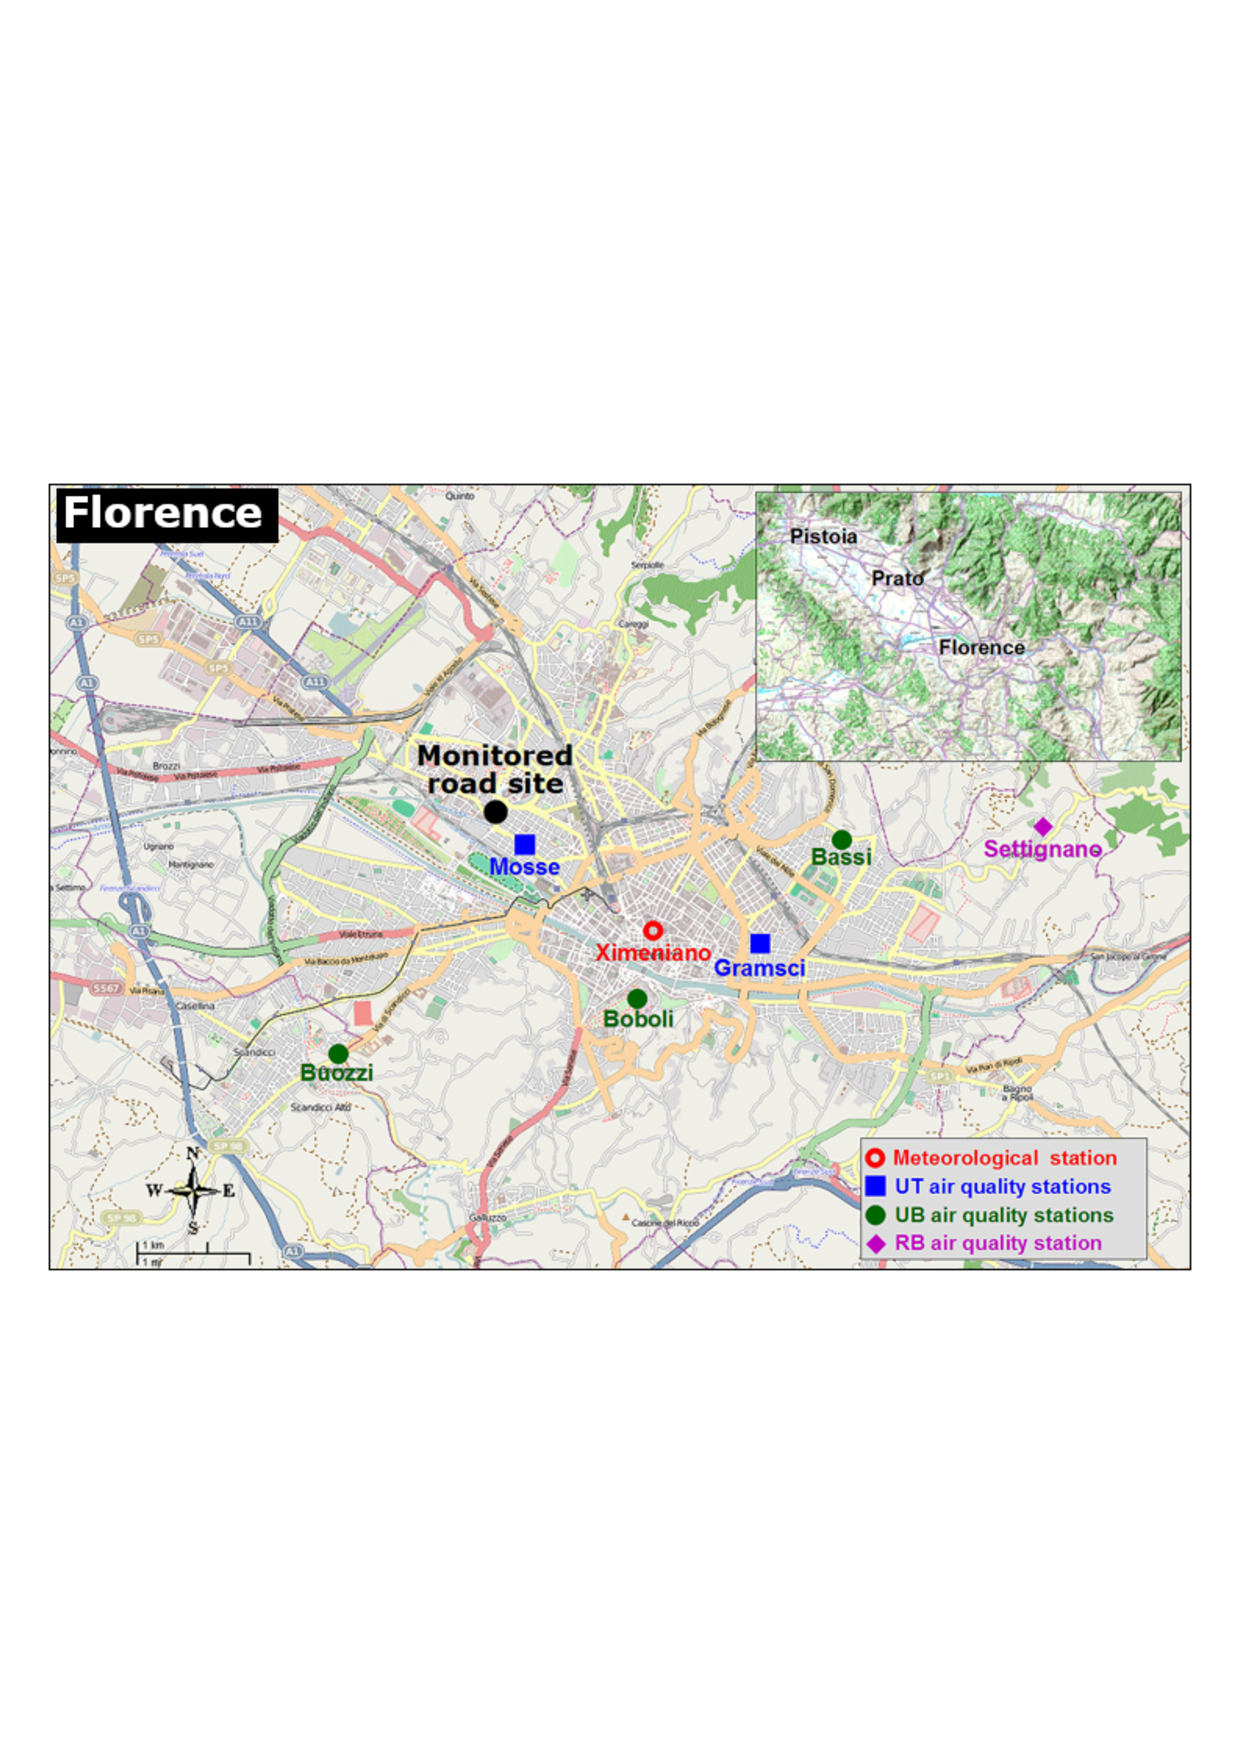
\includegraphics[width=\columnwidth]{FixStation01.png}
	\caption{Florence official air quality monitoring network.}
	\label{fig:floNet}
\end{figure} 
The main reason for using few sensors is represented by the cost; indeed, traditional air pollutant analyzers are
complicated, bulky and expensive, each instrument costing anywhere from
about five to tens of thousands Euro, accompanied by a significant amount
of resources required to routinely maintain and calibrate them.
However, fine resolution and air pollution data would serve as a powerful resource for understanding the pollution exposure levels and strategies to deal with them.
For this purpose, low-cost air quality sensors are an emerging technology and are now commercially available in a wide variety of designs and capabilities. 
In fact, the recent breakthrough of wireless sensor network technology opens the door to the possibility of
cost-effectively monitoring the concentration of pollutants via deployment of multiple low-cost sensors on the area of
interest. Such information can be further integrated with the one on traffic-induced air pollution, which indirectly comes
from real-time urban traffic monitoring systems, like the ones recently made available by the use of GPS devices (for
instance equipped on cellular and smart phones) as probe sensors for traffic flow.

This work has focused on the
study and development of an innovative air quality monitoring system able to monitor in real-time the concentration of
pollutants (gases and particle matters) in a complex urban environment by processing and fusing data coming from
different sources of information, including: point-wise measurements of pollutant concentration and of relevant
meteorological variables (such as wind speed, temperature, and humidity) collected from wireless sensors strategically
deployed in known locations over the area of interest; and aggregated data on the traffic flow provided by a real-time
traffic monitoring system. In the next sections, all the steps followed in the development of the proposed air quality monitoring system will be
described in some details. The developed monitoring systems has been validated on different scenarios involving both simulated and real data,
collected in two different measurement campaigns.

The rest of this paper is organized as follows.  Section 2 describes the adopted mathematical model of air pollutant diffusion and its discrete approximation based on the 
Finite Element Method (FEM). Section 3 presents the data assimilation techniques used to correct the simulated model on the basis of the available measurements.
Section 4 discusses the construction of the simulator of air pollutant diffusion as well as the methodology used for calculating the emissions associated with city traffic.
Section 5 presents the air quality sensors used in the two measurement campaigns described in Section 6. 
The results obtained with the developed air quality monitoring system in both simulated and real scenarios are provided in Sections 7 and 8, respectively.
Finally, concluding remarks are given in Section 9.

% The very first letter is a 2 line initial drop letter followed
% by the rest of the first word in caps.
% 
% form to use if the first word consists of a single letter:
% \IEEEPARstart{A}{demo} file is ....
% 
% form to use if you need the single drop letter followed by
% normal text (unknown if ever used by the IEEE):
% \IEEEPARstart{A}{}demo file is ....
% 
% Some journals put the first two words in caps:
% \IEEEPARstart{T}{his demo} file is ....
% 
% Here we have the typical use of a "T" for an initial drop letter
% and "HIS" in caps to complete the first word.
%\IEEEPARstart{T}{his} demo file is intended to serve as a ``starter file''
%for IEEE journal papers produced under \LaTeX\ using
%IEEEtran.cls version 1.8b and later.
%% You must have at least 2 lines in the paragraph with the drop letter
%% (should never be an issue)
%I wish you the best of success.
%
%\hfill mds
% 
%\hfill August 26, 2015
%
%\subsection{Subsection Heading Here}
%Subsection text here.

% needed in second column of first page if using \IEEEpubid
%\IEEEpubidadjcol

%\subsubsection{Subsubsection Heading Here}
%Subsubsection text here.
%

% An example of a floating figure using the graphicx package.
% Note that \label must occur AFTER (or within) \caption.
% For figures, \caption should occur after the \includegraphics.
% Note that IEEEtran v1.7 and later has special internal code that
% is designed to preserve the operation of \label within \caption
% even when the captionsoff option is in effect. However, because
% of issues like this, it may be the safest practice to put all your
% \label just after \caption rather than within \caption{}.
%
% Reminder: the "draftcls" or "draftclsnofoot", not "draft", class
% option should be used if it is desired that the figures are to be
% displayed while in draft mode.
%
%\begin{figure}[!t]
%\centering
%\includegraphics[width=2.5in]{myfigure}
% where an .eps filename suffix will be assumed under latex, 
% and a .pdf suffix will be assumed for pdflatex; or what has been declared
% via \DeclareGraphicsExtensions.
%\caption{Simulation results for the network.}
%\label{fig_sim}
%\end{figure}

% Note that the IEEE typically puts floats only at the top, even when this
% results in a large percentage of a column being occupied by floats.


% An example of a double column floating figure using two subfigures.
% (The subfig.sty package must be loaded for this to work.)
% The subfigure \label commands are set within each subfloat command,
% and the \label for the overall figure must come after \caption.
% \hfil is used as a separator to get equal spacing.
% Watch out that the combined width of all the subfigures on a 
% line do not exceed the text width or a line break will occur.
%
%\begin{figure*}[!t]
%\centering
%\subfloat[Case I]{\includegraphics[width=2.5in]{box}%
%\label{fig_first_case}}
%\hfil
%\subfloat[Case II]{\includegraphics[width=2.5in]{box}%
%\label{fig_second_case}}
%\caption{Simulation results for the network.}
%\label{fig_sim}
%\end{figure*}
%
% Note that often IEEE papers with subfigures do not employ subfigure
% captions (using the optional argument to \subfloat[]), but instead will
% reference/describe all of them (a), (b), etc., within the main caption.
% Be aware that for subfig.sty to generate the (a), (b), etc., subfigure
% labels, the optional argument to \subfloat must be present. If a
% subcaption is not desired, just leave its contents blank,
% e.g., \subfloat[].


% An example of a floating table. Note that, for IEEE style tables, the
% \caption command should come BEFORE the table and, given that table
% captions serve much like titles, are usually capitalized except for words
% such as a, an, and, as, at, but, by, for, in, nor, of, on, or, the, to
% and up, which are usually not capitalized unless they are the first or
% last word of the caption. Table text will default to \footnotesize as
% the IEEE normally uses this smaller font for tables.
% The \label must come after \caption as always.
%
%\begin{table}[!t]
%% increase table row spacing, adjust to taste
%\renewcommand{\arraystretch}{1.3}
% if using array.sty, it might be a good idea to tweak the value of
% \extrarowheight as needed to properly center the text within the cells
%\caption{An Example of a Table}
%\label{table_example}
%\centering
%% Some packages, such as MDW tools, offer better commands for making tables
%% than the plain LaTeX2e tabular which is used here.
%\begin{tabular}{|c||c|}
%\hline
%One & Two\\
%\hline
%Three & Four\\
%\hline
%\end{tabular}
%\end{table}


% Note that the IEEE does not put floats in the very first column
% - or typically anywhere on the first page for that matter. Also,
% in-text middle ("here") positioning is typically not used, but it
% is allowed and encouraged for Computer Society conferences (but
% not Computer Society journals). Most IEEE journals/conferences use
% top floats exclusively. 
% Note that, LaTeX2e, unlike IEEE journals/conferences, places
% footnotes above bottom floats. This can be corrected via the
% \fnbelowfloat command of the stfloats package.

%\section{Introducton}

\section{Air pollution modeling}

\subsection{Advection-diffusion-reaction model}
The diffusion of a pollutant in the environment can be described by a PDE of the form
	\be
	\displaystyle{\frac{\partial x}{\partial t}} +  \mathcal{A}(x) ~=~ f \,\,\,\,\, \mbox{in } \Omega
	\label{PDE}
	\ee
	with possibly inhomogeneous boundary condition
	\be
	\mathcal B (x) ~=~ g \,\,\,\, \mbox{ on } \partial \Omega\, .
	\label{boundary}
	\ee
	where:
	$x(\mb{p},t)$ is the space-time dependent scalar field of interest (e.g. concentration, temperature), defined over the space-time domain
	$\Omega \times \mathbb{R}$; 
	the space domain $\Omega$ is supposed to be bounded and with smooth boundary $ \partial \Omega$; 
	$\mb{p} \in \Omega$ denotes the $d$-dimensional ($d \in \{ 1, 2, 3 \}$) position vector;
	$t \in \mathbb{R}$ denotes time;
	$\mathcal{A}(\cdot)$ and $\mathcal{B}(\cdot)$ are the \textit{advection-diffusion} and, respectively, \textit{Robin} operators defined as
	\[
	\mathcal{A}(x) = - \lambda \nabla^2 x + \mb{v}^T \nabla x 
	\] 
	and 
	\[
	\mathcal{B}(x) =  {\partial x}/{\partial \mb{n}} + \beta x
	\]
	%\begin{eqnarray}
	%\mathcal{A}(x) & \defi & - \lambda \nabla^2 x + \mb{v}^T \nabla x 
	%\label{a-d} \\
	%\mathcal{B}(x) & \defi & {\partial x}/{\partial \mb{n}} + \beta x;
	%\end{eqnarray}
	$\lambda$ is the diffusion coefficient;
	$\mb{v}(\mb{p})$ is the advection velocity vector;
	$\beta(\mb{p}) \geq 0$ is a, possibly space-dependent, coefficient; 
	$ {\partial x}/{\partial \mb{n}} = \mb{n}^T \nabla x$,
	$\mb{n}$ being the outward pointing unit normal vector of the boundary 
	$\partial \Omega$;
	$g(\mb{p},t)$ is the forcing term  acting on the boundary $\partial \Omega$.
	The term $f(\mb{p},t)$ represents the internal sources of pollution.
	 
	The aim is to estimate the continuous field $x(\mb{p},t)$ given measurements
	\be
	y_{k,i} ~=~  x \left( \mb{s}_i (t_k), t_k \right)  + v_{k,i}
	\label{meas}
	\ee
	provided by sensors $i \in \mathcal{S} \defi \{ 1, \dots, S \}$, located at positions $\mb{s}_i (t_k) \in \Omega$, at discrete sampling instants $t_k$, $k \in
	\Z_+ = \{ 1, 2, \dots \}$, such that $0 < t_1 < t_2 < \cdots$. The sensor positions are allowed to be time-varying in order to account also for mobile sensors.
	
	The above stated dynamic estimation problem is clearly infinite-dimensional.
	It will be shown in the next section how it can be approximated into a finite-dimensional one by exploiting the \textit{finite element} (FE) method.
	

\subsection{Finite-element spatial discretization}
The PDE (\ref{PDE}) with boundary condition (\ref{boundary}) can be recast into the
	following integral form:
	\[
	\int_\Omega \frac{\partial x}{\partial t} \varphi \, d\mb{p} \, - \,
	\lambda \int_\Omega ~\nabla^2 x~ \varphi \, d\mb{p} +
	\int_\Omega \mb{v}^T  ~\nabla x~ \varphi \, d\mb{p} =
	\int_\Omega f \varphi \, d\mb{p}
	\]
	where $\varphi(\mb{p})$ is a generic space-dependent weight function. 
	By applying Green's identity and thanks to (\ref{boundary}),
	one obtains:
	%	\begin{multline}
	%	\int_\Omega \frac{\partial x}{\partial t} \varphi \, d\mb{p} + \lambda
	%	\int_\Omega \nabla^T x ~\nabla \varphi \, d\mb{p} +
	%	\int_\Omega \mb{v}^T  \nabla x ~\varphi \, d\mb{p} 
	%	\\ - \lambda
	%	\int_{\partial \Omega} \frac{\partial x}{\partial \mb{n}} \varphi \, 
	%	d\mb{p}
	%	=
	%	\int_\Omega f \, \varphi  \,d\mb{p} 
	%	\end{multline}
	%	where,  the boundary integral reverts to
	\begin{multline} \nonumber
	\int_\Omega \frac{\partial x}{\partial t} \, \varphi \, d\mb{p} + \lambda
	\int_\Omega \nabla^T x  \nabla \varphi \, d\mb{p} +
	\int_\Omega \mb{v}^T  ~\nabla x ~\varphi \, d\mb{p} 
	\\  -
	\lambda \int_{\partial \Omega} \left( 
	g -\beta x \right) \varphi \, d\mb{p} 
	=
	\int_\Omega f \, \varphi \, d\mb{p}
	\end{multline}
	By subdividing the domain $\Omega$ into a suitable set of non overlapping
	elements and by defining a suitable set of basis functions
	$\phi_{j} (\mb{p})$,  $j=1,\ldots,n$, on them, it is possible to write an
	approximation of the unknown function $x(\mb{p},t)$ as
	\be
	x(\mb{p},t) = \sum_{j=1}^{n} \phi_{j}(\mb{p}) \, x_j(t) ~=~ \boldsymbol{\phi}^T(\mb{p}) \, \mb{x}(t)
	\label{EXPA}
	\ee
	where: $x_j(t)$ is the unknown expansion coefficient of function $x(\mb{p},t)$
	relative to time $t$ and basis function $\phi_j(\mb{p})$; $\bs{\phi}(\mb{p}) 
	\defi col \{ \phi_j (\mb{p} ) \}_{j=1}^n$ and $\mb{x}(t) \defi col \{ x_j(t)
	\}_{j=1}^n$.
	
	The choices of the basis functions $\phi_{j}$ and of the elements are key
	points of the FE method. Typically, the elements (triangles or quadrilaterals
	in 2D, polyhedral in 3D) define a FE mesh with vertices $\mb{p}_j \in \Omega,
	j=1,\ldots,n $.
	Then each basis function $\phi_{j}$ is a piece-wise polynomial which vanishes
	outside the FEs around $\mb{p}_j$ and such that $\phi_{j}(\mb{p}_i) =
	\delta_{ij}$, $\delta_{ij}$ denoting the Kronecker delta.
	
	By choosing the test function $\varphi$ equal to the selected basis functions, the Galerkin
	weighted residual method is applied and the following equation is obtained
	\cite{Pelosi09}
	
	\begin{multline} \label{WF}
	\small{\underbrace{\left[ \int_\Omega  
			\bs{\phi}(\mb{p}) \,\bs{\phi}^T(\mb{p}) d\mb{p} 
			\right]}_{\mb{M}} \dot{\mb{x}}(t)  + 
		\underbrace{\left[ \lambda \int_\Omega 
			\nabla	\bs{\phi}(\mb{p}) \,\nabla \bs{\phi}^T(\mb{p}) d\mb{p} 
			\right]}_{\mb{S}_\lambda} \mb{x}(t) }\\
\small{+ \underbrace{\left[ \int_\Omega 
			\bs{\phi}(\mb{p}) ~ \mb{v}^T(\mb{p}) \,\nabla \bs{\phi}^T(\mb{p}) \, d\mb{p} 
			\right]}_{\mb{G}} \mb{x}(t) }
		\\
	\small{+ \underbrace{\left[ \lambda \int_{\partial \Omega} 
			\beta(\mb{p}) \, \bs{\phi}(\mb{p}) \,\bs{\phi}^T(\mb{p}) \, d\mb{p}
			\right]}_{\mb{Q}_\beta} \mb{x}(t) = }\\
	=  \small{\underbrace{\left[\displaystyle{\int_\Omega} \bs{\phi}(\mb{p})
			\bs{\phi}(\mb{p})^T d\mb{p}	\right]}_{\mb{Q}_f} {\mb{u}}(t) 
		+  \underbrace{\left[ \lambda \int_{\partial \Omega} 
			\bs{\phi}(\mb{p}) \,\bs{\phi}^T(\mb{p}) d\mb{p}
			\right] }_{\mb{Q}_g} {\mb{g}}(t) }
	\end{multline} 
	where in the integrals on the contour $\partial \Omega$ it is assumed that
	the various functions are the restrictions to $\partial \Omega$ of the original
	functions defined over $\Omega$, and that for $f(\mb{p},t)$ and $g(\mb{p},t)$
	expansions akin to (\ref{EXPA}) hold, i.e.
	\begin{eqnarray*}g(\mb{p},t) &=& \sum_{j=1}^{n} \phi_{j}(\mb{p}) \,  g_j(t) ~=~
	\boldsymbol{\phi}^T(\mb{p}) \, {\mb{g}}(t) \\
	f(\mb{p},t) &=& \sum_{j=1}^{n} \phi_{j}(\mb{p}) \, f_j(t) ~=~
	\boldsymbol{\phi}^T(\mb{p}) \, {\mb{f}}(t) 
	\end{eqnarray*}
	
	It is evident how all integrals in the LHS (\ref{WF}) depend only on basis functions
	and can be computed {\em a priori}. 
	In particular, the first two integrals yields the well known \textit{mass} and
	\textit{stiffness} matrices $\mb{M}$ and $\mb{S}_\lambda$ \cite{Pelosi09}.
	Matrices $\mb{G}$, $\mb{Q}_\beta$ , $\mb{Q}_f$, and $\mb{Q}_g$
	are non standard but can be easily computed in simplex coordinates for first
	order triangular elements \cite{Pelosi09,Silv96}.
	
	Then, by regularly discretizing in time (\ref{WF}) with sampling interval $\Delta $ (i.e. $t_k = k \, \Delta$) and approximating the time
	derivative with the finite difference  $\dot{\mb{x}}(t)\simeq
	(\mb{x}_{k+1}-\mb{x}_k)/\Delta$, the following discrete-time linear descriptor system is
	obtained:
	\begin{multline}
	\mb{M}\left(\frac{\mb{x}_{k+1}-\mb{x}_k}{\Delta}\right) +
	\mb{S}_\lambda \mb{x}_{k+1}  + \mb{G}\mb{x}_{k+1} + \mb{Q}_\beta\mb{x}_{k+1} \simeq
	 \mb{Q}_{f} {\mb{f}}_{k+1}+ \\
	  \mb{Q}_{g} {\mb{g}}_{k+1}
	\label{dt-desc-sys}
	\end{multline}
	which can be rewritten as
	\begin{equation}\label{eq:descriptor}
	\left ( \mb{S} + \frac{\mb{M}}{\Delta} \right ) \mb{x}_{k+1} = \frac{\mb{M}}{\Delta}  \mb{x}_{k} + \mb{u}_k + \mb{w}_k
	\end{equation}
	where $\mb{S} = \mb{S}_\lambda + \mb{G} + \mb{Q}_\beta $, $\mb{u}_k =  \mb{Q}_{f} {\mb{f}}_{k+1}+ \mb{Q}_{g} {\mb{g}}_{k+1}$ and
	$\mb{w}_k$ is a process disturbance taking into account also the space-time discretization errors. 
	From (\ref{eq:descriptor}), one obtains the discrete-time model
	\be 
	\mb{x}_{k+1} = \mb{A}\mb{x}_k + \mb{B}   \mb{u}_{k} + \mb{B}   \mb{w}_k 
	\label{dt-sys}
	\ee
	where
	\[
	\begin{aligned}\label{eq:A}
	\mb{A} =  \left ( \mb{S} + \frac{\mb{M}}{\Delta} \right )^{-1} \frac{\mb{M}}{\Delta}  , \quad \mb{B} = \left ( \mb{S} + \frac{\mb{M}}{\Delta} \right )^{-1} \, .
	\end{aligned}
	\]
	
	\begin{remark}
	Notice that in the case of Dirichlet boundary conditions of the form $x =g$ on $\partial \Omega$, equations analogous to (\ref{eq:descriptor})
	and (\ref{dt-sys}) can be obtained provided that $\mb{S}$ and $\mb{u}_k$ are suitably redefined. Further, the considered model can be easily extended 
	so as to account for the presence of a reactive term in the linear operator $\mathcal A (x)$ and for space-time dependent diffusion coefficient $\lambda$,
	giving rise to the general model $\mathcal{A}(x) = - \nabla \cdot (\lambda \nabla x) + \mb{v}^T \nabla x + r x$.
	\end{remark}
	
	Clearly, in the above model, the following elements and parameters have to be specified:
	\begin{itemize}
	\item The geometry on which the Finite Element Method (FEM) method is applied, i.e. the domain $\Omega$ and the mesh nodes $\textbf{p}$, must be chosen both to define the models 
	and plan the measurement 		campaigns.
	\item The forcing term $f$ and the boundary values $g$, that determine the values of $\textbf{u}_k$  must be tuned according to the vehicle emission rates 
	and the pollutant concentration on the boundary nodes.
	\item The value of the diffusion coefficient $\lambda$ for various pollutants can be taken from the literature \cite{Massman_001}.
	\item The advection vector $\mb{v}$, representing the wind velocity, can be found for any geographical area in Italy from the web site source \textit{ilmeteo.it}.
	\end{itemize}
	The construction of the considered model is described in some details in Section 4.
	
	In accordance with the above-described model, let $\mathcal S_k \subseteq \mathcal S $ be the subset of sensors collecting a measurement at the discrete-time instant
	$t_k$, then the measurement equation takes the form
	\begin{equation}\label{eq:y}
	\mb {y}_k = \mb{C}_k \mb{x}_k + \mb{v}_k
	\end{equation}
	where, 
	\begin{eqnarray*}
	&&\mb{y}_k \defi col \left\{ y_{k,i} \right\}_{i\in \mathcal{S}_k},  \quad \mb{v}_k \defi col \left\{ v_{k,i} \right\}_{i \in \mathcal{S}_k}, \\
	&& \mb{C}_k = col \left\{ \bs{\phi}^T(\mb{s}_i (t_k)) \right\}_{i \in \mathcal{S}_k}
	\end{eqnarray*}
	

\subsection{Time-discretization}
Then, by regularly discretizing in time (\ref{WF}) with sampling interval $\Delta $ (i.e. $t_k = k \, \Delta$) and approximating the time
	derivative with the finite difference  $\dot{\mb{x}}(t)\simeq
	(\mb{x}_{k+1}-\mb{x}_k)/\Delta$, the following discrete-time linear descriptor system is
	obtained:
	\begin{multline}
	\mb{M}\left(\frac{\mb{x}_{k+1}-\mb{x}_k}{\Delta}\right) +
	\mb{S}_\lambda \mb{x}_{k+1}  + \mb{G}\mb{x}_{k+1} + \mb{Q}_\beta\mb{x}_{k+1} \simeq
	 \mb{Q}_{f} {\mb{f}}_{k+1}+ \mb{Q}_{g} {\mb{g}}_{k+1}
	\label{dt-desc-sys}
	\end{multline}
	which can be rewritten as
	\begin{equation}\label{eq:descriptor}
	\left ( \mb{S} + \frac{\mb{M}}{\Delta} \right ) \mb{x}_{k+1} = \frac{\mb{M}}{\Delta}  \mb{x}_{k} + \mb{u}_k + \mb{w}_k
	\end{equation}
	where $\mb{S} = \mb{S}_\lambda + \mb{G} + \mb{Q}_\beta $, $\mb{u}_k =  \mb{Q}_{f} {\mb{f}}_{k+1}+ \mb{Q}_{g} {\mb{g}}_{k+1}$ and
	$\mb{w}_k$ is a process disturbance taking into account also the space-time discretization errors. 
	From (\ref{eq:descriptor}), one obtains the discrete-time model
	\be 
	\mb{x}_{k+1} = \mb{A}\mb{x}_k + \mb{B}   \mb{u}_{k} + \mb{B}   \mb{w}_k 
	\label{dt-sys}
	\ee
	where
	\[
	\begin{aligned}\label{eq:A}
	\mb{A} =  \left ( \mb{S} + \frac{\mb{M}}{\Delta} \right )^{-1} \frac{\mb{M}}{\Delta}  , \quad \mb{B} = \left ( \mb{S} + \frac{\mb{M}}{\Delta} \right )^{-1} \, .
	\end{aligned}
	\]
	
	\begin{remark}
	Notice that in the case of Dirichlet boundary conditions of the form $x =g$ on $\partial \Omega$, equations analogous to (\ref{eq:descriptor})
	and (\ref{dt-sys}) can be obtained provided that $\mb{S}$ and $\mb{u}_k$ are suitably redefined. Further, the considered model can be easily extended 
	so as to account for the presence of a reactive term in the linear operator $\mathcal A (x)$ and for space-time dependent diffusion coefficient $\lambda$,
	giving rise to the general model $\mathcal{A}(x) = - \nabla \cdot (\lambda \nabla x) + \mb{v}^T \nabla x + r x$.
	\end{remark}
	
	Clearly, in the above model, the following elements and parameters have to be specified:
	\begin{itemize}
	\item The geometry on which the Finite Element Method (FEM) method is applied, i.e. the domain $\Omega$ and the mesh nodes $\textbf{p}$, must be chosen both to define the models 
	and plan the measurement 		campaigns.
	\item The forcing term $f$ and the boundary values $g$, that determine the values of $\textbf{u}_k$  must be tuned according to the vehicle emission rates 
	and the pollutant concentration on the boundary nodes.
	\item The value of the diffusion coefficient $\lambda$ for various pollutants can be taken from the literature \cite{Massman_001}.
	\item The advection vector $\mb{v}$, representing the wind velocity, can be found for any geographical area in Italy from the web site source \textit{ilmeteo.it}.
	\end{itemize}
	The construction of the considered model is described in some details in Section 4.
	
	In accordance with the above-described model, let $\mathcal S_k \subseteq \mathcal S $ be the subset of sensors collecting a measurement at the discrete-time instant
	$t_k$, then the measurement equation takes the form
	\begin{equation}\label{eq:y}
	\mb {y}_k = \mb{C}_k \mb{x}_k + \mb{v}_k
	\end{equation}
	where, 
	\begin{eqnarray*}
	&&\mb{y}_k \defi col \left\{ y_{k,i} \right\}_{i\in \mathcal{S}_k},  \quad \mb{v}_k \defi col \left\{ v_{k,i} \right\}_{i \in \mathcal{S}_k}, \\
	&& \mb{C}_k = col \left\{ \bs{\phi}^T(\mb{s}_i (t_k)) \right\}_{i \in \mathcal{S}_k}
	\end{eqnarray*}

\subsection{Use of meteo and vehicular traffic data for parameter tuning and emissions calculation}
In a complex scenario such as a modern urban center, the main contribution to pollution is certainly due to city traffic.
Traffic-related air pollution is a serious problem with significant health impacts in both urban and suburban environments. Hot emissions are the emissions produced when the engine and the pollution control systems
of the vehicle (e.g. catalyst) have reached their normal operating temperature. Following \cite{bib:MEET001}, they can be
calculated if the emission per unit of activity and the total activity over the reference time scale are known, using the formula:
\begin{equation} \label{hot_emission}
E_{hot} = e\cdot m
\end{equation}
where: $E_{hot}$ is the hot emission factor, in units of mass per unit of time (usually in [$g\cdot veh/h$]);
$e$ is the emission factor in [$g/km$];
 $m$ is the activity, in distance travelled per time unit (usually in [$km\cdot veh/h$]).

The activity $m$ required for the emission calculation according to equation \eqref{hot_emission} is defined as:
\begin{equation} \label{activity_eq}
m = n\cdot l
\end{equation}
where:
$n$ is the number of vehicles in each vehicle category;
 $l$ is the average speed of the amount of vehicles in each vehicle category, on each type of road.

Combining equations \eqref{hot_emission} and \eqref{activity_eq}, and taking into account the different vehicle
categories and the different types of road, the final equation for hot emission estimation can be derived for each type of pollutant:
\begin{equation} \label{emission_hot_pollutant}
E_k = \sum\limits_{i=1}^{n_c} n_i\hspace{0.3mm} l_i \sum\limits_{j=1}^{n_p} p_{i,j}\hspace{0.3mm} e_{i,j,k}
\end{equation}
where:
 $k$\hspace{0.8mm}identifies the pollutant;
 $i$\hspace{0.8mm}identifies the vehicle category;
 $j$\hspace{0.8mm}identifies the type of road;
 $n_i$\hspace{0.8mm}is the number of vehicles in category $i$;
 $l_i$\hspace{0.8mm}is the average speed of vehicle in category $i$;
 $p_{i,j}$\hspace{0.8mm}is the percentage of vehicles in each category $i$, travelling on road type $j$;
$e_{i,j,k}$\hspace{0.8mm}is the emission factor of pollutant $k$ corresponding to the average speed on road type $j$, for vehicle category $i$;
 $n_c$ is the number of vehicle categories;
 $n_p$ is the number of road types.

%-------------------------------------


In an urban area the streets can be considered of the same type (i.e. urban road). Moreover, for the activity \eqref{emission_hot_pollutant}, the following equivalence holds
\be
n\cdot l = h \cdot d
\ee \\
where: 
$h$ is the vehicle flow on each type of road;
$d$ is the total length of all roads belonging to a certain category of road types. 

Then, \eqref{emission_hot_pollutant} can be written in the following, simplified form:
\be
E_k = d\hspace{0.3mm} \sum\limits_{i=1}^{n_c}\hspace{0.1mm} h_i\hspace{0.5mm}  p_{i}\hspace{0.5mm} e_{i,k}
\ee
where:
 $k$\hspace{0.8mm}identifies the pollutant;
 $i$\hspace{0.8mm}identifies the vehicle category;
 $h_i$ \hspace{0.8mm}is the average vehicle flow in the urban roads in category $i$;
 $d$\hspace{0.8mm}is the total length of the amount of urban roads in a certain area considered area;
 $p_{i,j}$\hspace{0.8mm}is the percentage of vehicles in each category $i$;
$e_{i,k}$\hspace{0.8mm}is the emission factor of pollutant $k$ corresponding to the average speed on urban road type, for vehicle category $i$;
 $n_c$\hspace{0.8mm}is the number of vehicles categories.

Since generally the concentration of the pollutants is expressed in $\mu g/m^3$ or in $mg/m^3$ and each subdomain in road geometry shown in Figure \ref{fig:mesh_2} has its own pollutant concentration because of the difference of traffic intensity, the hot emission in each road subsection is calculated as follows:
\be \label{eq:authorknow}
E_{vol,k}^{sub} = \dfrac{d^{sub}}{vol^{sub}}\hspace{0.3mm} \sum\limits_{i=1}^{n_c}\hspace{0.1mm} h_{i}^{sub}\hspace{0.3mm}  p_{i}\hspace{0.3mm} e_{i,k}
\ee
where $d^{sub}$ is the lenght of the road subsection, $h_{i}^{sub}$  is its vehicle flow and $vol^{sub}$ is a volume corresponding to the area of the same subsection multiplied by a height dimensioned in the order of tens of meters. \\
The emission factors have been derived using data from engine test-bed measurements. Each engine has been
categorised according to the type of vehicle in which it is used. There are four categories of vehicles chosen to represent the \textit{car fleet} of the city of Florence, available from the \textit{ACI (Automobile Club d'Italia)} website: \textit{passenger cars}, \textit{trucks} or \textit{heavy goods vehicles} (HGVs), \textit{urban buses} and \textit{mopeds}.
The method for calculating the emission factor for the first vehicle category is shown in the Tables \ref{tab:speed_dep_gpassengercars} and \ref{tab:TabEmPassCarCo} and depends on the type of pollutant \cite{bib:MEET001}.
%%%%%%%%%%%TABLE
\begin{table}[tbp]
 \centering
 \begin{center}  
  \begin{tabular}{c}
   % \begin{center}                                                                         
\hspace{-3.5mm}      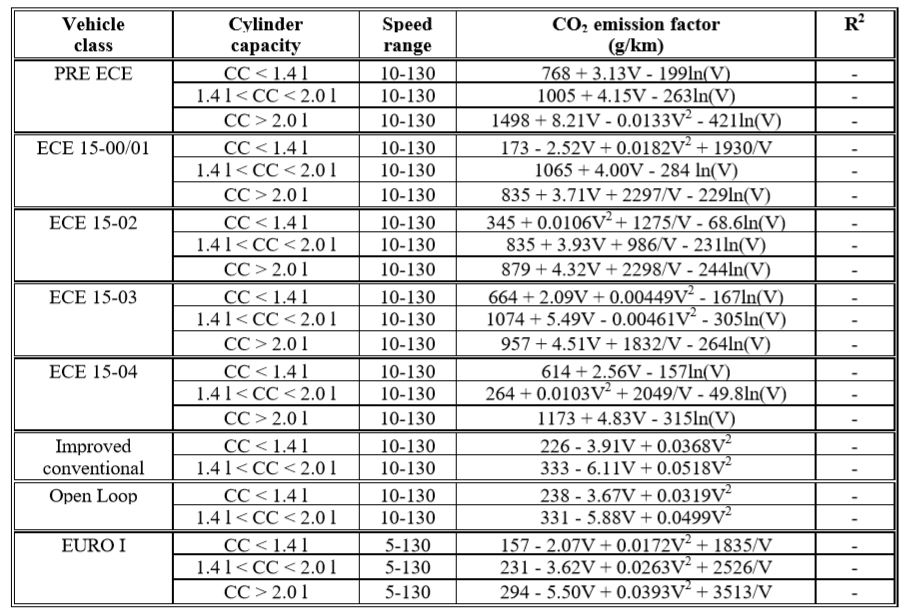
\includegraphics[width=0.5\textwidth]{figure/Emission_passvehicle_co2.jpg} 
    %\end{center}     
  \end{tabular}
\end{center}  
\caption{\textit{Courtesy of Transport Research Laboratory (TRL)} \cite{bib:MEET001}\\Speed dependency of carbon dioxide emission factors for gasoline passenger cars.}
  \label{tab:speed_dep_gpassengercars}
\end{table}
%%%%%%%END TABLE
%%%%%%%%%%%TABLE
\begin{table}[tbp]
 \centering
 \begin{center}  
  \begin{tabular}{c}
   % \begin{center}                                                                         
      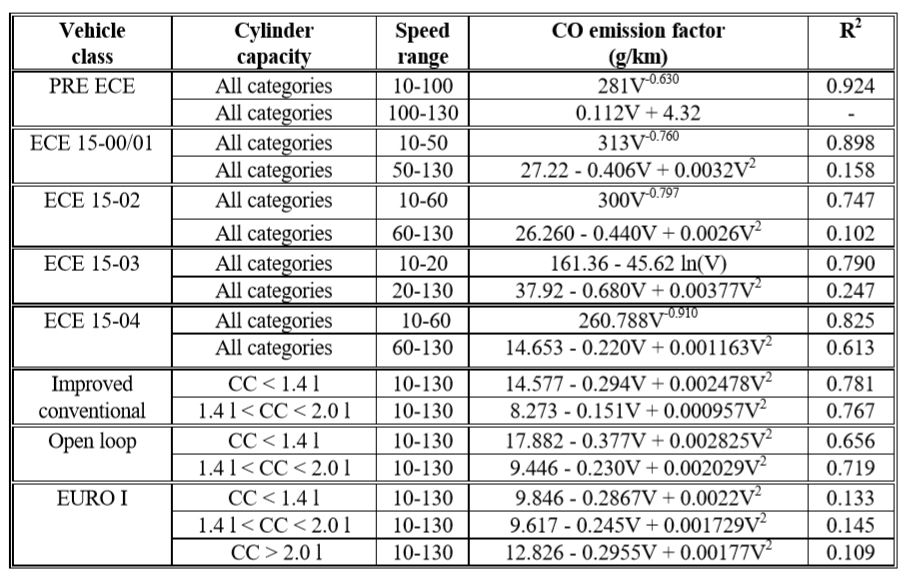
\includegraphics[width=0.5\textwidth]{figure/Emission_passvehicle_co.jpg}
    %\end{center}     
  \end{tabular}
\end{center}  
\caption{\textit{Courtesy of Transport Research Laboratory (TRL)} \cite{bib:MEET001}\\Speed dependency of CO emission factors for gasoline passenger cars.}
  \label{tab:TabEmPassCarCo}
\end{table}
%%%%%%%%%%END DOUBLE TABLE
 For the second and third vehicle category the following formula has been used:

\begin{equation}
\varepsilon_{pc} = K_{pc} + a_{pc}v + b_{pc}v^2 + c_{pc}v^3 + \dfrac{d_{pc}}{v} + \dfrac{e_{pc}}{v^2} + \dfrac{f_{pc}}{v^3}
\end{equation}
where: $\varepsilon_{pc}$ is the emission factor;
$K_{pc}$ is a constant;
$a_{pc}$ - $f_{pc}$ are coefficients;
$v$ is the mean velocity of the vehicle.


As seen in the first category, the values of the coefficients depend again on the type of pollutant, but in this case they depend also on each gross vehicle weight; for this reason it has been assumed HGVs having a gross vehicle weight from 3.5 to 7.5 tons. For HGVs and urban buses the values of the coefficients are shown in Tables \ref{tab:hgv} and \ref{tab:urbanbus} respectively.
%%%%%%%%%%%TABLE
\begin{table}[tbp]
 \centering
 \begin{center}  
  \begin{tabular}{c}
   % \begin{center}                                                                         
      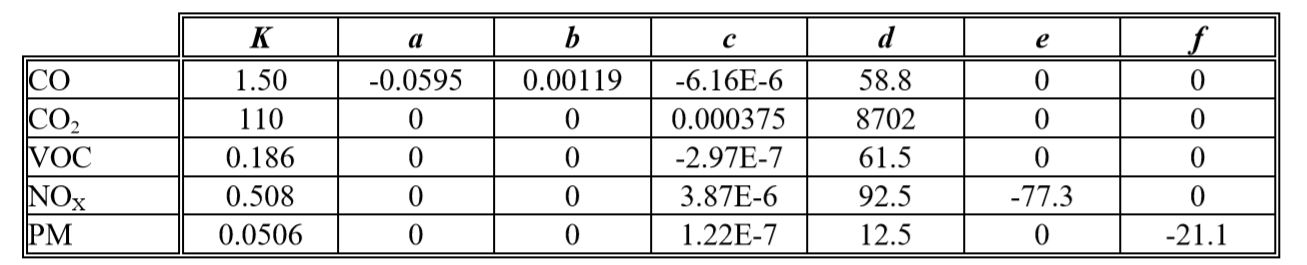
\includegraphics[width=0.5\textwidth]{figure/tab_coef_hgv.jpg} 
    %\end{center}     
  \end{tabular}
\end{center}  
\caption{\textit{Courtesy of Transport Research Laboratory (TRL)} \cite{bib:MEET001}\\ Coefficients of emission functions for heavy goods vehicles with gross vehicle weights from 3.5 to 7.5 tonnes.}
  \label{tab:hgv}
\end{table}
%%%%%%%END TABLE
%%%%%%%%%%%TABLE
\begin{table}[tbp]
 \centering
 \begin{center}  
  \begin{tabular}{c}
   % \begin{center}                                                                         
      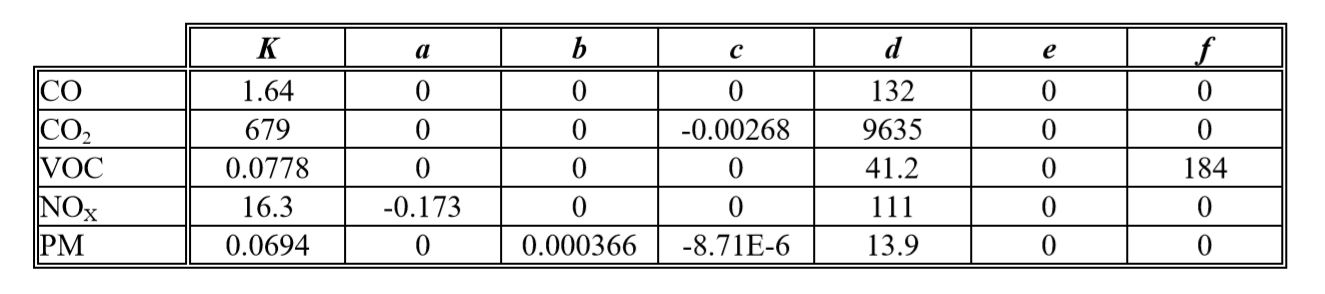
\includegraphics[width=0.5\textwidth]{figure/tab_coef_uBuses.jpg}
    %\end{center}     
  \end{tabular}
\end{center}  
\caption{\textit{Courtesy of Transport Research Laboratory (TRL)} \cite{bib:MEET001}\\Coefficients of emission functions for urban buses.}
  \label{tab:urbanbus}
\end{table}
%%%%%%%%%%END DOUBLE TABLE
Finally, for mopeds, the emission factors are presented in Table \ref{tab:mopeds}. \\
%%%%%%%%%%%TABLE
\begin{table}[tbp]
 \centering
 \begin{center}  
  \begin{tabular}{c}
   % \begin{center}                                                                         
      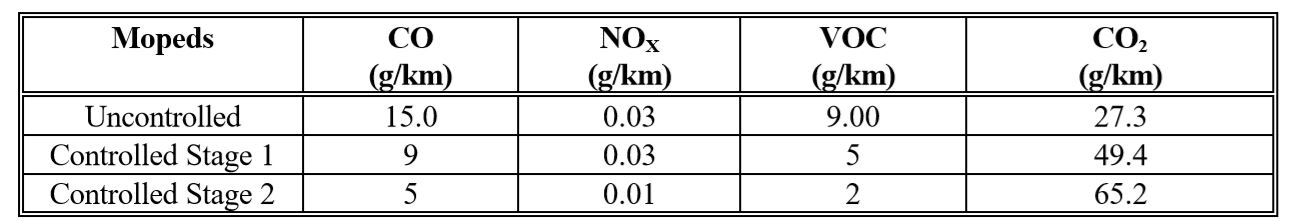
\includegraphics[width=0.5\textwidth]{figure/tab_mopeds_ef.jpg}
    %\end{center}     
  \end{tabular}
\end{center}  
\caption{\textit{Courtesy of Transport Research Laboratory (TRL)} \cite{bib:MEET001}\\ Emission factors for mopeds.}
  \label{tab:mopeds}
\end{table}
%%%%%%%%%%END DOUBLE TABLE
As it is clear from the expressions in the tables presented in this section, the calculation of the average speed and the flow of vehicles in each category is required for obtaining the emission factors in urban roads.
In this respect, \textit{levels of service (LOS)} to classify the vehicle flow and the average speed have been identified, as shown in Tables \ref{tab:flow} and \ref{tab:flowvelocity} \cite{bib:neuralgasindian}.
%%%%%%%%%%%TABLE
\begin{table}[tbp]
 \centering
 \begin{center}  
  \begin{tabular}{c}
   % \begin{center}                                                                         
      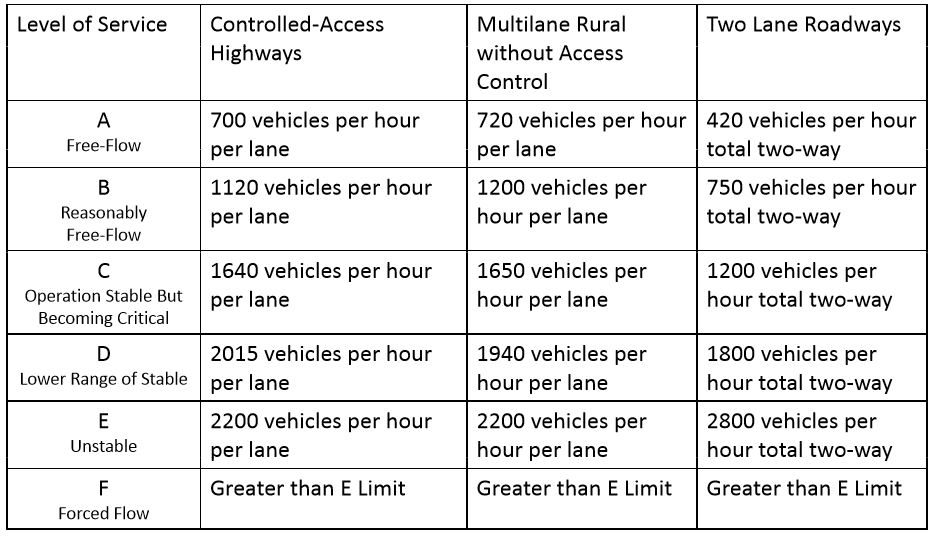
\includegraphics[width=0.45\textwidth]{figure/fig_traffic_flow.jpg}
    %\end{center}     
  \end{tabular}
\end{center}  
\caption{Flow rate limits classified as levels of service.}
  \label{tab:flow}
\end{table}
%%%%%%%%%%END DOUBLE TABLE
%%%%%%%%%%%TABLE
\begin{table}[tbp]
 \centering
 \begin{center}  
  \begin{tabular}{c}
   % \begin{center}                                                                         
      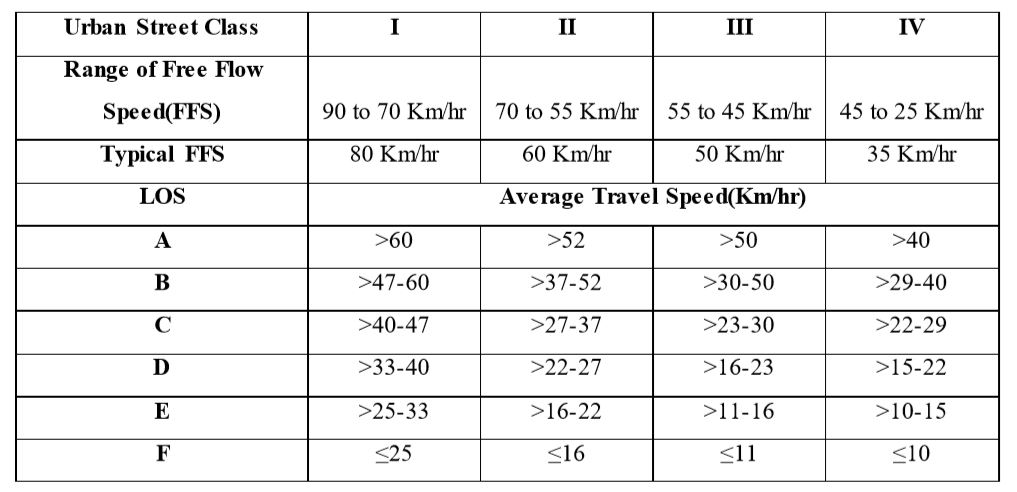
\includegraphics[width=0.457\textwidth]{figure/fig_urban_gas.jpg}
    %\end{center}     
  \end{tabular}
\end{center}  
\caption{\textit{Courtesy of IOSR Journal of Engineering (IOSRJEN)} \cite{bib:neuralgasindian}\\ Urban speed ranges for different LOS proposed in Indian conditions by neural gas Clustering method.} 
  \label{tab:flowvelocity}
\end{table}
%%%%%%%%%%END DOUBLE TABLE
This information has been used to define four emission classes, each one associated with a different color, corresponding to a traffic intensity in the maps provided by the \textit{ArcGis} platform.
%figure
\begin{figure}[tbp]
	\centering
%\hspace*{-0.2cm}   
	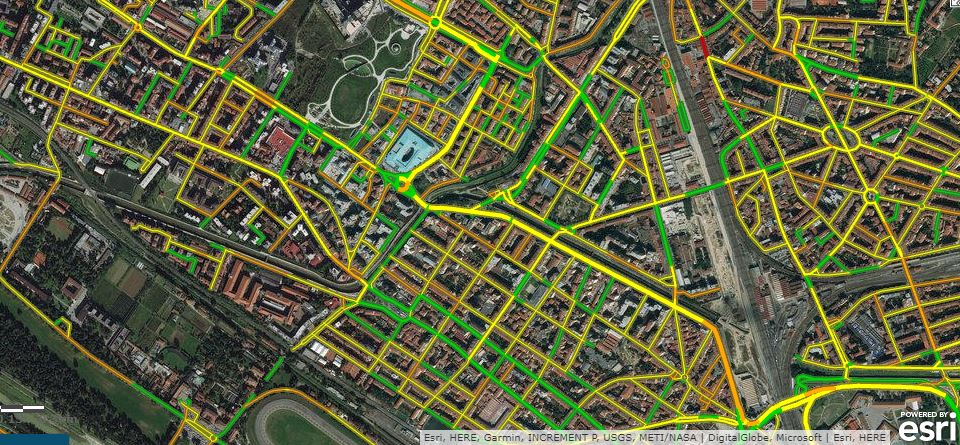
\includegraphics[width=0.48\textwidth]{figure/fig_traffic_arcgis.jpg}
	\caption{Traffic layer on a \textit{Esri} map available from the ArcGis website, including the polluted area of interest in Novoli, Florence.}
	\label{fig:arcgis}
         % \end{center}
\end{figure}
%\vspace{0.5mm}
%end figure
This application, as shown in Figure \ref{fig:arcgis}, yields, in real-time, the traffic intensity of any geographical urban area of the world where this information is represented as a map with four different colors; in ascending order of traffic intensity, respectively, green, yellow, orange and red. \\
Thus, by associating this information to each subdomain of the road network, an estimation of the emission rate $h$ of each internal node of the mesh shown in Figure \ref{fig:geom_mesh} has been obtained. 
In turn, such estimate has been used to construct the vector of internal emissions $\mb{f}_{k+1}$ and, hence, the vector of exogenous inputs $\mb{u}_k$ in model
(\ref{eq:descriptor}).

\section{Finite-element state estimation for large-scale systems}
To obtain a good estimate of the pollutant concentration in real-time, a mathematical description that models the transport dynamics of pollutants is not sufficient. Indeed, all mathematical models are 
		affected by uncertainties of different type with respect to the true system. For this reason, in the environmental monitoring systems a data assimilation component is required, aimed at integrating the 
		basic model with data collected over the field, i.e. the area of interest.
		Thanks to the finite element approximation described in the previous section, the original infinite-dimensional continuous-time filtering problem can 
	be reduced to a much simpler finite-dimensional (albeit large-scale) discrete time linear filtering problem.
		The most efficient algorithm used in  data assimilation problems, in the case of linear systems such as (\ref{dt-sys})-(\ref{eq:y}),  is undoubtedly the Kalman filter. 
	
	Thanks to the finite element approximation described in the previous section, the original infinite-dimensional continuous-time filtering problem can 
	be reduced to a much simpler finite-dimensional (albeit large-scale) discrete time linear filtering problem.
	The resulting filter recursion becomes:
	\begin{eqnarray}
	&& \hspace{-.8cm} \mb{\hat{x}}_{k|k} = \left \{
	\ba{ll}
	\mb{\hat{x}}_{k|k-1} + \mb{L}_k
	\left( \mb{y}_k - \mb{h} \left( \mb{\hat{x}}_{k|k-1} \right) \right) & \mbox{ if } \mathcal S_k \ne \emptyset \\
	\mb{\hat{x}}_{k|k-1}  & \mbox{ otherwise }
	\ea \right . \nonumber \\
	&&  \hspace{-.8cm} \mb{P}_{k|k} = \left \{
	\ba{ll}
	\mb{P}_{k|k-1} - \mb{L}_k  
	\mb{C}_k^T \mb{P}_{k|k-1} \quad \quad \quad \quad & \mbox{ if } \mathcal S_k \ne \emptyset  \\
	\mb{P}_{k|k-1}   & \mbox{ otherwise }
	\ea \right . \nonumber \\
	&& \hspace{-.8cm} \mb{\hat{x}}_{k+1|k}  =  \mb{A} \mb{\hat{x}}_{k|k} + \mb{B} \mb{u}_k \nonumber \\
	&& \hspace{-.8cm} \mb{P}_{k+1|k}  =  \mb{A} \mb{P}_{k|k} \mb{A}^T + \mb{Q}_k \label{KF}
	\end{eqnarray}
	where $ \mb{L}_k$ is the Kalman filter gain
	\begin{eqnarray}
			&& \mb{L}_k  =  \mb{P}_{k|k-1} \mb{C}_k \left( \mb{R}_k + \mb{C}_k \mb{P}_{k|k-1} \mb{C}_k^T \right)^{-1} \label{Gain}
	\end{eqnarray}
	used to correct the prediction $\mb{\hat{x}}_{k|k-1}$  on the basis of the collected measurements $\mathcal S_k$. Of course the correction is applied only
	for $k$ such that $\mathcal S_k \ne \emptyset $ (i.e., when at least one of the sensors is active). 
	The recursion is initialized from suitable $\mb{\hat{x}}_{1|0}$ and $\mb{P}_{1|0} = \mb{P}_{1|0}^T > \mb{0}$.
	In (\ref{KF}), $\mb{Q}_k$ and $\mb{R}_k$ denote the covariance matrices of the process noise $\mb{B} \mb{w}_k$ and, respectively, measurement noise $\mb{v}_k$.

	Notice that the process noise $\mb{w}_k$ arises from the superposition of several uncertainties and/or perturbations (including, e.g., the FE approximation of the continuous field) so that its whiteness  
	and uncorrelation with the initial state, usually assumed in a stochastic framework, do not hold true in practice.
	As a result, the Kalman filter algorithm (\ref{KF})-(\ref{Gain}) looses its Bayes optimality bus still preserves deterministic least-squares optimality as the minimizer
	of the following cost function
	$$\ba{rcl}
	 J & = & \left( \mb{x}-\mb{\hat{x}}_{1|0} \right)^T \mb{P}_{1|0}^{-1}  \left( \mb{x}-\mb{\hat{x}}_{1|0} \right) + \\
	 & & \displaystyle{\sum_{i=1}^{k-1}}  \left( \mb{x}_{i+1} - \mb{A} \mb{x}_i \right)^T \mb{Q}_i^{-1}   \left( \mb{x}_{i+1} - \mb{A} \mb{x}_i \right) +  \\
	 &&  \displaystyle{\sum_{i=1}^{k}}  \left( \mb{y}_{i} - \mb{C} \mb{x}_i \right)^T \mb{R}_i^{-1}   \left( \mb{y}_{i} - \mb{C} \mb{x}_i \right)	 
	 \ea
	$$


	\subsection{Ensemble Kalman Filter}
	
	The problem of the Kalman filter described in the previous section is the computational cost necessary to carry out real-time environmental monitoring activities that imply large data processing 
	and consequently high computational costs. In fact, as will be detailed in Section 4, the state space model  (\ref{dt-sys})-(\ref{eq:y})  arising from the space-time discretization of the original PDE 
	is a large-scale system involving thousands of state variables.
	For this reason, to process all the data and generate the estimates, we have used a variant of the Kalman filter known as \textit{ensemble Kalman filter} (EnKF), able to provide 
	a substantial reduction of the computational burden while retaining good filtering performance.
	
	The ensemble Kalman filter (EnKF) is a suboptimal estimator, where the error statistics are predicted by using Monte Carlo or ensemble integration. The EnkF method is presented in three stages. First, to represent the error statistics in the forecast step, we assume that at time $k$, we have an ensemble of $q$ forecasted state estimates with random sample errors. We denote this ensemble as $\mb{X}_{k}^{f} \in \mathbb{R}^{n\times q}$, where
\begin{align}
\mb{X}_{k}^{f} \overset{\Delta}{=} (\textbf{x}_{k}^{f_{1}},\dots,\textbf{x}_{k}^{f_{q}}),
\end{align}
and the superscript $f_{i}$ refers to the $i$-th forecast ensemble member. Then, the ensemble mean $\overline{\mb{x}}_{k}^{f} \in \mathbb{R}^{n}$ is defined as
\begin{align} \label{eq:mean_state_forecast}
\overline{\mb{x}}_{k}^{f} \overset{\Delta}{=} \dfrac{1}{q}\sum_{i=1}^{q}\mb{x}_{k}^{f_{i}} \ \, .
\end{align}
Since the true state $\mb{x}_{k}$ is not known, we approximate the estimation error statistics by using the ensemble members. We define the ensemble error matrix $\mb{E}_{k}^{f} \in \mathbb{R}^{n\times q}$ around the ensemble mean as
\begin{align} \label{eq:ensmatr1}
\mb{E}_{k}^{f} \overset{\Delta}{=} \big[ \textbf{x}_{k}^{f_{1}} - \overline{\mb{x}}_{k}^{f},\dots,\textbf{x}_{k}^{f_{q}} - \overline{\mb{x}}_{k}^{f} \big]
\end{align}
and the ensemble of output error $\mb{E}_{y_{k}}^{f} \in \mathbb{R}^{p\times q}$ by
\begin{align}
\mb{E}_{y_{k}}^{f} \overset{\Delta}{=} \big[ \textbf{y}_{k}^{f_{1}} - \overline{\mb{y}}_{k}^{f},\dots,\textbf{y}_{k}^{f_{q}} - \overline{\mb{y}}_{k}^{f} \big] \ \, .
\end{align}
We then approximate $\mb{P}_{k}^{f}$ by $\hat{\mb{P}}_{k}^{f}$, $\mb{P}_{{xy}_{k}}^{f}$ by $\hat{\mb{P}}_{{xy}_{k}}^{f}$ and $\mb{P}_{{yy}_{k}}^{f}$ by $\hat{\mb{P}}_{{yy}_{k}}^{f}$, respectively, where
\be
\begin{aligned}
\hat{\mb{P}}_{k}^{f} \overset{\Delta}{=} \dfrac{1}{q-1\footnotemark}&\sum_{i=1}^{q}\mb{E}_{k}^{f}(\mb{E}_{k}^{f})^{\mathrm{T}} \ \, , \\
\hat{\mb{P}}_{{xy}_{k}}^{f} \overset{\Delta}{=} \dfrac{1}{q-1}\sum_{i=1}^{q}\mb{E}_{k}^{f}(\mb{E}_{{xy}_{k}}^{f})^{\mathrm{T}} \ \, &, \ \
\hat{\mb{P}}_{{yy}_{k}}^{f} \overset{\Delta}{=} \dfrac{1}{q-1}\sum_{i=1}^{q}\mb{E}_{{y}_{k}}^{f}(\mb{E}_{{y}_{k}}^{f})^{\mathrm{T}} \ \,
\end{aligned} 
%\footnotetext{The use of the term $q-1$ instead $q$ in the formula for the sample covariance, sample variance and sample standard deviation is called Bessel's correction. This method corrects the bias in the estimation of the population variance. It also partially corrects the bias in the estimation of the population standard deviation. However, the correction often increases the mean squared error in these estimates. This technique is named after Friedrich Bessel.}
\ee
Thus, we interpret the forecast ensemble mean as the best forecast estimate of the state, and the spread of the ensemble members around the mean as the error between the best estimate and the actual state. \\
The second step is the analysis step to be performed whenever $\mathcal S_k \ne \emptyset$: to obtain the analysis estimates of the state, the EnKF performs an ensemble of parallel data assimilation cycles, where for $i = 1,\dotsc ,q$
\begin{align} \label{eq:correctionstep03}
\textbf{x}_{k}^{{a}_{i}} &= \textbf{x}_{k}^{{f}_{i}} + \hat{\mb{L}}_{k}(\textbf{y}_{k}^{i} - \mb{C}_k \, \textbf{x}_{k}^{{f}_{i}}) \ \, . 
\end{align}
The \textit{perturbed observations} $\mb{y}_{k}^{i}$ are given by
\begin{align} \label{eq:pertobs02}
\mb{y}_{k}^{i} = \mb{y}_{k} + \mb{v}_{k}^{i} \ \, , 
\end{align}
where $\mb{v}_{k}^{i}$ is a zeo-random variable with a normal distribution and covariance $\mb{R}_{k}$. The sample error covariance matrix computed from the $\mb{v}_{k}^{i}$ converges to $\mb{R}_{k}$ as $q\xrightarrow{}\infty$. We approximate the analysis error covariance $\mb{P}_{k}^{a}$ by $\hat{\mb{P}}_{k}^{a}$, where
\begin{align}
\hat{\mb{P}}_{k}^{a} \overset{\Delta}{=} \dfrac{1}{q-1}&\sum_{i=1}^{q}\mb{E}_{k}^{a}(\mb{E}_{k}^{a})^{\mathrm{T}} \ \, ,
\end{align}
and $\mb{E}_{k}^{a}$ is defined by \eqref{eq:ensmatr1} with $\textbf{x}_{k}^{{f}_{i}}$ replaced by $\textbf{x}_{k}^{{a}_{i}}$ and $\overline{\mb{x}}_{k}^{f}$ replaced by the mean of the analysis estimate ensemble members. We use the classical Kalman filter gain expression and the approximations of the error covariances to determine the filter gain $\hat{\mb{L}}_{k}$ by
\begin{align}
\hat{\mb{L}}_{k} = \hat{\mb{P}}_{{xy}_{k}}^{f}(\hat{\mb{P}}_{{yy}_{k}}^{f})^{-1} \ \, .
\end{align}
The last step is the prediction of error statistics in the forecast step:
\begin{equation}\label{eq:pred}
\mb{x}_{k+1}^{{f}_{i}} = \mb{A} \mb{x}_{k}^{{a}_{i}} + \mb{w}_{k}^{i} \ \, ,
\end{equation}
where the values $\mb{w}_{k}^{i}$ are sampled from a normal distribution with average zero and covariance $\mb{Q}_{k}$. The sample error covariance matrix computed from the $\mb{w}_{k}^{i}$ converges to $\mb{Q}_{k}$ as $q\xrightarrow{}\infty$. 

Concerning equation (\ref{eq:pred}), it is worth noting that computation of the matrix $\mb{A}$ involves the inversion of a large scale matrix and hence is prone to numerical errors.
Further, while the matrices $\mb{M}$ and $\mb{S}$ are sparse thanks to the structure of the FEM approximation, the matrix $\mb{A}$ loses this desirable property due to the inversion in
(\ref{eq:A}). Hence, in practice it is better to avoid computing $\mb{A}$ and instead use directly the descriptor model (\ref{eq:descriptor}) in the computation of the predicted error statistics.
Hence, at each time instant and for any $i$, the following linear system of equations has to be solved with respect to  $\mb{x}_{k+1}^{{f}_{i}} $
\be
\bigg(\mb{S} + \dfrac{\mb{M}}{\Delta}\bigg) \mb{x}_{k+1}^{{f}_{i}} = \bigg( \dfrac{\mb{M}}{\Delta}\mb{x}_{k}^{{a}_{i}} + \textbf{u}_{k}\bigg)  + \mb{w}_{k}^{i}
\ee


The resulting filtering recursion is summarized in Algorithm \ref{alg:2}.


\begin{algorithm}[t!]
\caption{FEM Ensemble Kalman Filter}
\begin{algorithmic} \label{alg:2}
\STATE \textbf{Initial Data}: The ensemble size $q > 0$ and the prior estimate $\hat{\mb{x}}_{1|0} = \overline{\mb{x}}_{1}^{f}$. 
\STATE \textbf{Initial Step}:
\STATE  Draw the samples $\mb{X}_{1}^{f} \overset{\Delta}{=} (\textbf{x}_{1}^{f_{1}},\dots,\textbf{x}_{1}^{f_{q}})$ from the prior estimate $\hat{\mb{x}}_{1|0}$ such that $\textbf{x}_{1}^{f_{i}}\sim\mathcal{N}(\hat{\mb{x}}_{1|0},\mb{Q}_{k})$, for $i=1,\dots,q$, 
 \STATE compute the measurements $\mb{y}_{1}^{f_i} = \mb{h}(\textbf{x}_{1}^{f_{i}})$, for $i=1,\dots,q$, 
 \STATE compute the mean measurement $\overline{\mb{y}}_{1}^{f} = \dfrac{1}{q}\sum_{i=1}^{q}\mb{y}_{1}^{f_{i}}$, 
 \STATE compute the prior ensemble matrices $\mb{E}_{1}^{f}$ and $\mb{E}_{{y}_1}^{f}$.
\STATE  \textbf{for} $k=1,2,\dots$ \textbf{do}: 
\STATE\hspace{.5cm} \textbf{Step 1 (\textit{Correction step}}): 
\STATE\hspace{.5cm} set $\hat{\mb{P}}_{{xy}_{k}}^{f} = \dfrac{1}{q-1}\sum_{i=1}^{q}\mb{E}_{k}^{f}(\mb{E}_{{y}_k}^{f})^{\mathrm{T}}$,
\STATE\hspace{.5cm} set $\hat{\mb{P}}_{{yy}_{k}}^{f} = \dfrac{1}{q-1}\sum_{i=1}^{q}\mb{E}_{{y}_k}^{f}(\mb{E}_{{y}_k}^{f})^{\mathrm{T}}$,
\STATE\hspace{.5cm} set $\hat{\mb{L}}_{k} = \hat{\mb{P}}_{{xy}_{k}}^{f}(\hat{\mb{P}}_{{yy}_{k}}^{f})^{-1}$,
\STATE\hspace{.5cm} draw $\textbf{v}_{k}^{i}\sim\mathcal{N}(0,\mb{R}_{k})$, for $i=1,\dots,q$,
\STATE\hspace{.5cm} set $\textbf{x}_{k}^{{a}_{i}} = \textbf{x}_{k}^{{f}_{i}} + \hat{\mb{L}}_{k}(\textbf{y}_{k} + \textbf{v}_{k}^{i} - \mb{C}_k \, \textbf{x}_{k}^{{f}_{i}})$, for $i=1,\dots,q$, \ \ \mbox{({data update})} 
\STATE\hspace{.5cm} set $\hat{\mb{x}}_{k|k} \overset{\Delta}{=} \overline{\mb{x}}_{k}^{a} = \dfrac{1}{q}\sum_{i=1}^{q}\mb{x}_{k}^{a_{i}}$,
\STATE\hspace{.5cm} set $\mb{E}_{k}^{a} = \big[ \textbf{x}_{k}^{a_{1}} - \overline{\mb{x}}_{k}^{a},\dots,\textbf{x}_{k}^{a_{q}} - \overline{\mb{x}}_{k}^{a} \big]$, \ \ \, (optional)
\STATE\hspace{.5cm} set $\hat{\mb{P}}_{k}^{a} = \dfrac{1}{q-1}\sum_{i=1}^{q}\mb{E}_{k}^{a}(\mb{E}_{k}^{a})^{\mathrm{T}}$, \ \ \, (optional) 
%%%%%%%%%%%%%%%%
\STATE\hspace{.5cm}   \textbf{Step 2 (\textit{Prediction step}}):
\STATE\hspace{.5cm} draw $\mb{w}_{k}^{i}\sim\mathcal{N}(0,\mb{Q}_{k})$, for $i=1,\dots,q$,
\STATE\hspace{.5cm} compute $\mb{x}_{k+1}^{{f}_{i}} $ by solving the system of linear equations \\ $\quad \quad \bigg(\mb{S} + \dfrac{\mb{M}}{\Delta}\bigg) \mb{x}_{k+1}^{{f}_{i}} = \bigg( \dfrac{\mb{M}}{\Delta}\mb{x}_{k}^{{a}_{i}} + \textbf{u}_{k}\bigg)  + \mb{w}_{k}^{i}$, for $i=1,\dots,q$, %$\mb{x}_{k+1}^{{f}_{i}} = \mb{f}(\mb{x}_{k}^{{a}_{i}}, \mb{u}_{k}) + \mb{w}_{k}^{i}$, for $i=1,\dots,q$, 
\STATE\hspace{.5cm} set $\hat{\mb{x}}_{k+1|k} \overset{\Delta}{=} \overline{\mb{x}}_{k+1}^{f} = \dfrac{1}{q}\sum_{i=1}^{q}\mb{x}_{k+1}^{f_{i}}$,
\STATE\hspace{.5cm} set $\mb{E}_{k+1}^{f} = \big[ \textbf{x}_{k+1}^{f_{1}} - \overline{\mb{x}}_{k+1}^{f},\dots,\textbf{x}_{k+1}^{f_{q}} - \overline{\mb{x}}_{k+1}^{f} \big]$,
\STATE\hspace{.5cm} set $\mb{y}_{k+1}^{f_i} = \mb{C}_{k+1} \textbf{x}_{k+1}^{f_{i}}$, for $i=1,\dots,q$, 
\STATE\hspace{.5cm} set $\overline{\mb{y}}_{k+1}^{f} = \dfrac{1}{q}\sum_{i=1}^{q}\mb{y}_{k+1}^{f_{i}}$,
\STATE\hspace{.5cm} set $\mb{E}_{{y}_{k+1}}^{f} = \big[ \textbf{y}_{k+1}^{f_{1}} - \overline{\mb{y}}_{k+1}^{f},\dots,\textbf{y}_{k+1}^{f_{q}} - \overline{\mb{y}}_{k+1}^{f} \big]$.
%%%%%%%%%%%%%%%%%%%%%%%%%%%%%%
\STATE \textbf{end for}
\end{algorithmic}
\end{algorithm}

\begin{remark}
Note that the Kalman filter recursion involves computation of the predicted covariance $\mb{P}_{k+1|k} \in \mathbb{R}^{n\times n}$, which requires $\mathcal{O}(n^{3})$ operation where $n = {\rm dim}(\mb{x})$. On the contrary for the EnKF,  only $\hat{\mb{P}}_{{xy}_{k}}^{f}$ and $\hat{\mb{P}}_{{yy}_{k}}^{f}$,are evaluated, requiring $\mathcal{O}(pqn)$ operation
where $p ={\rm dim} (\mb{y})$. Hence, if $q\ll n$, then the computational burden of evaluating the approximate covariances in the EnKF is much less than the computational burden of determining the  covariances in the EKF. 
\end{remark}
	

\section{Air-quality sensors}
Recent air quality regulations (Directive 2008/50/EC) enforce the transition from point-based monitoring networks to new tools that must be capable of mapping and forecasting air quality on the totality of land area, and therefore the totality of citizens. This implies that new tools, such as models and additional indicative measurements, are needed in addition to accurate fixed air quality monitoring stations, that until now have been taken as reference by local administrators for the enforcement of various mitigation strategies. However, due to their sporadic spatial distribution, they cannot describe the high spatial pollutant variations within cities. Integrating additional indicative measurements may provide adequate information on the spatial distribution of air quality parameters. For this purpose, new low-cost and small size sensors are becoming available to be employed in air quality monitoring including mobile applications. 
It was precisely the use of this type of sensor that has allowed the acquisition of pollutant concentration measurements in the field to be used later (offline) for data assimilation. 
In particular we used \textit{AirQino}, a compact low-cost air quality monitoring station by the Insitute of Biometorology-Italian National Research Council (IBIMET-CNR). AirQino  is based on an Arduino Shield Compatible electronic board and integrated with low-cost and high resolution industrial \textit{Strain Measurement Devices} (SMD), dedicated to monitoring environmental parameters and air quality pollutants  (humidity, temperature, CO, CO$_2$, O$_3$, NO$_2$, VOC, PM2.5, PM10) in urban environment. The board also incorporates a microprocessor unit that acquires all the installed sensor data. Sensors transmit geolocated data through the General Packet Radio Service (GPRS) technology to a data server connected to the applications and web server allowing to display observations in real-time on a web browser \cite{bib:alicavphd06}. The board is placed into an IP68 waterproof box as shown in Figure \ref{fig:ip68_image}. Because the gases monitored by the AirQino sensor board includes also reactive ones, airflow inside the waterproof box is designed to minimize the gas interference. Furthermore, a small brushless fan blows the air out of the box. 
This creates a depression that attracts air from the inlet window. 


%%%%%%%%%%%%%%%%%%%%%%%%%%%%%%%%%
\begin{figure}[tbp] 
	\centering
	\subfloat[]{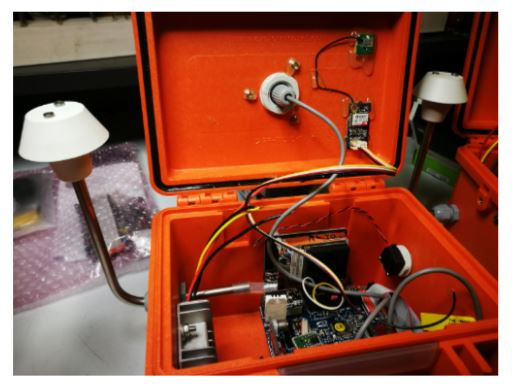
\includegraphics[width=.48\columnwidth]{figure/fig_sensor_ip68_1.jpg}
		\label{fig:nodes_triangle_2D}}
	\hfill
	\subfloat[]{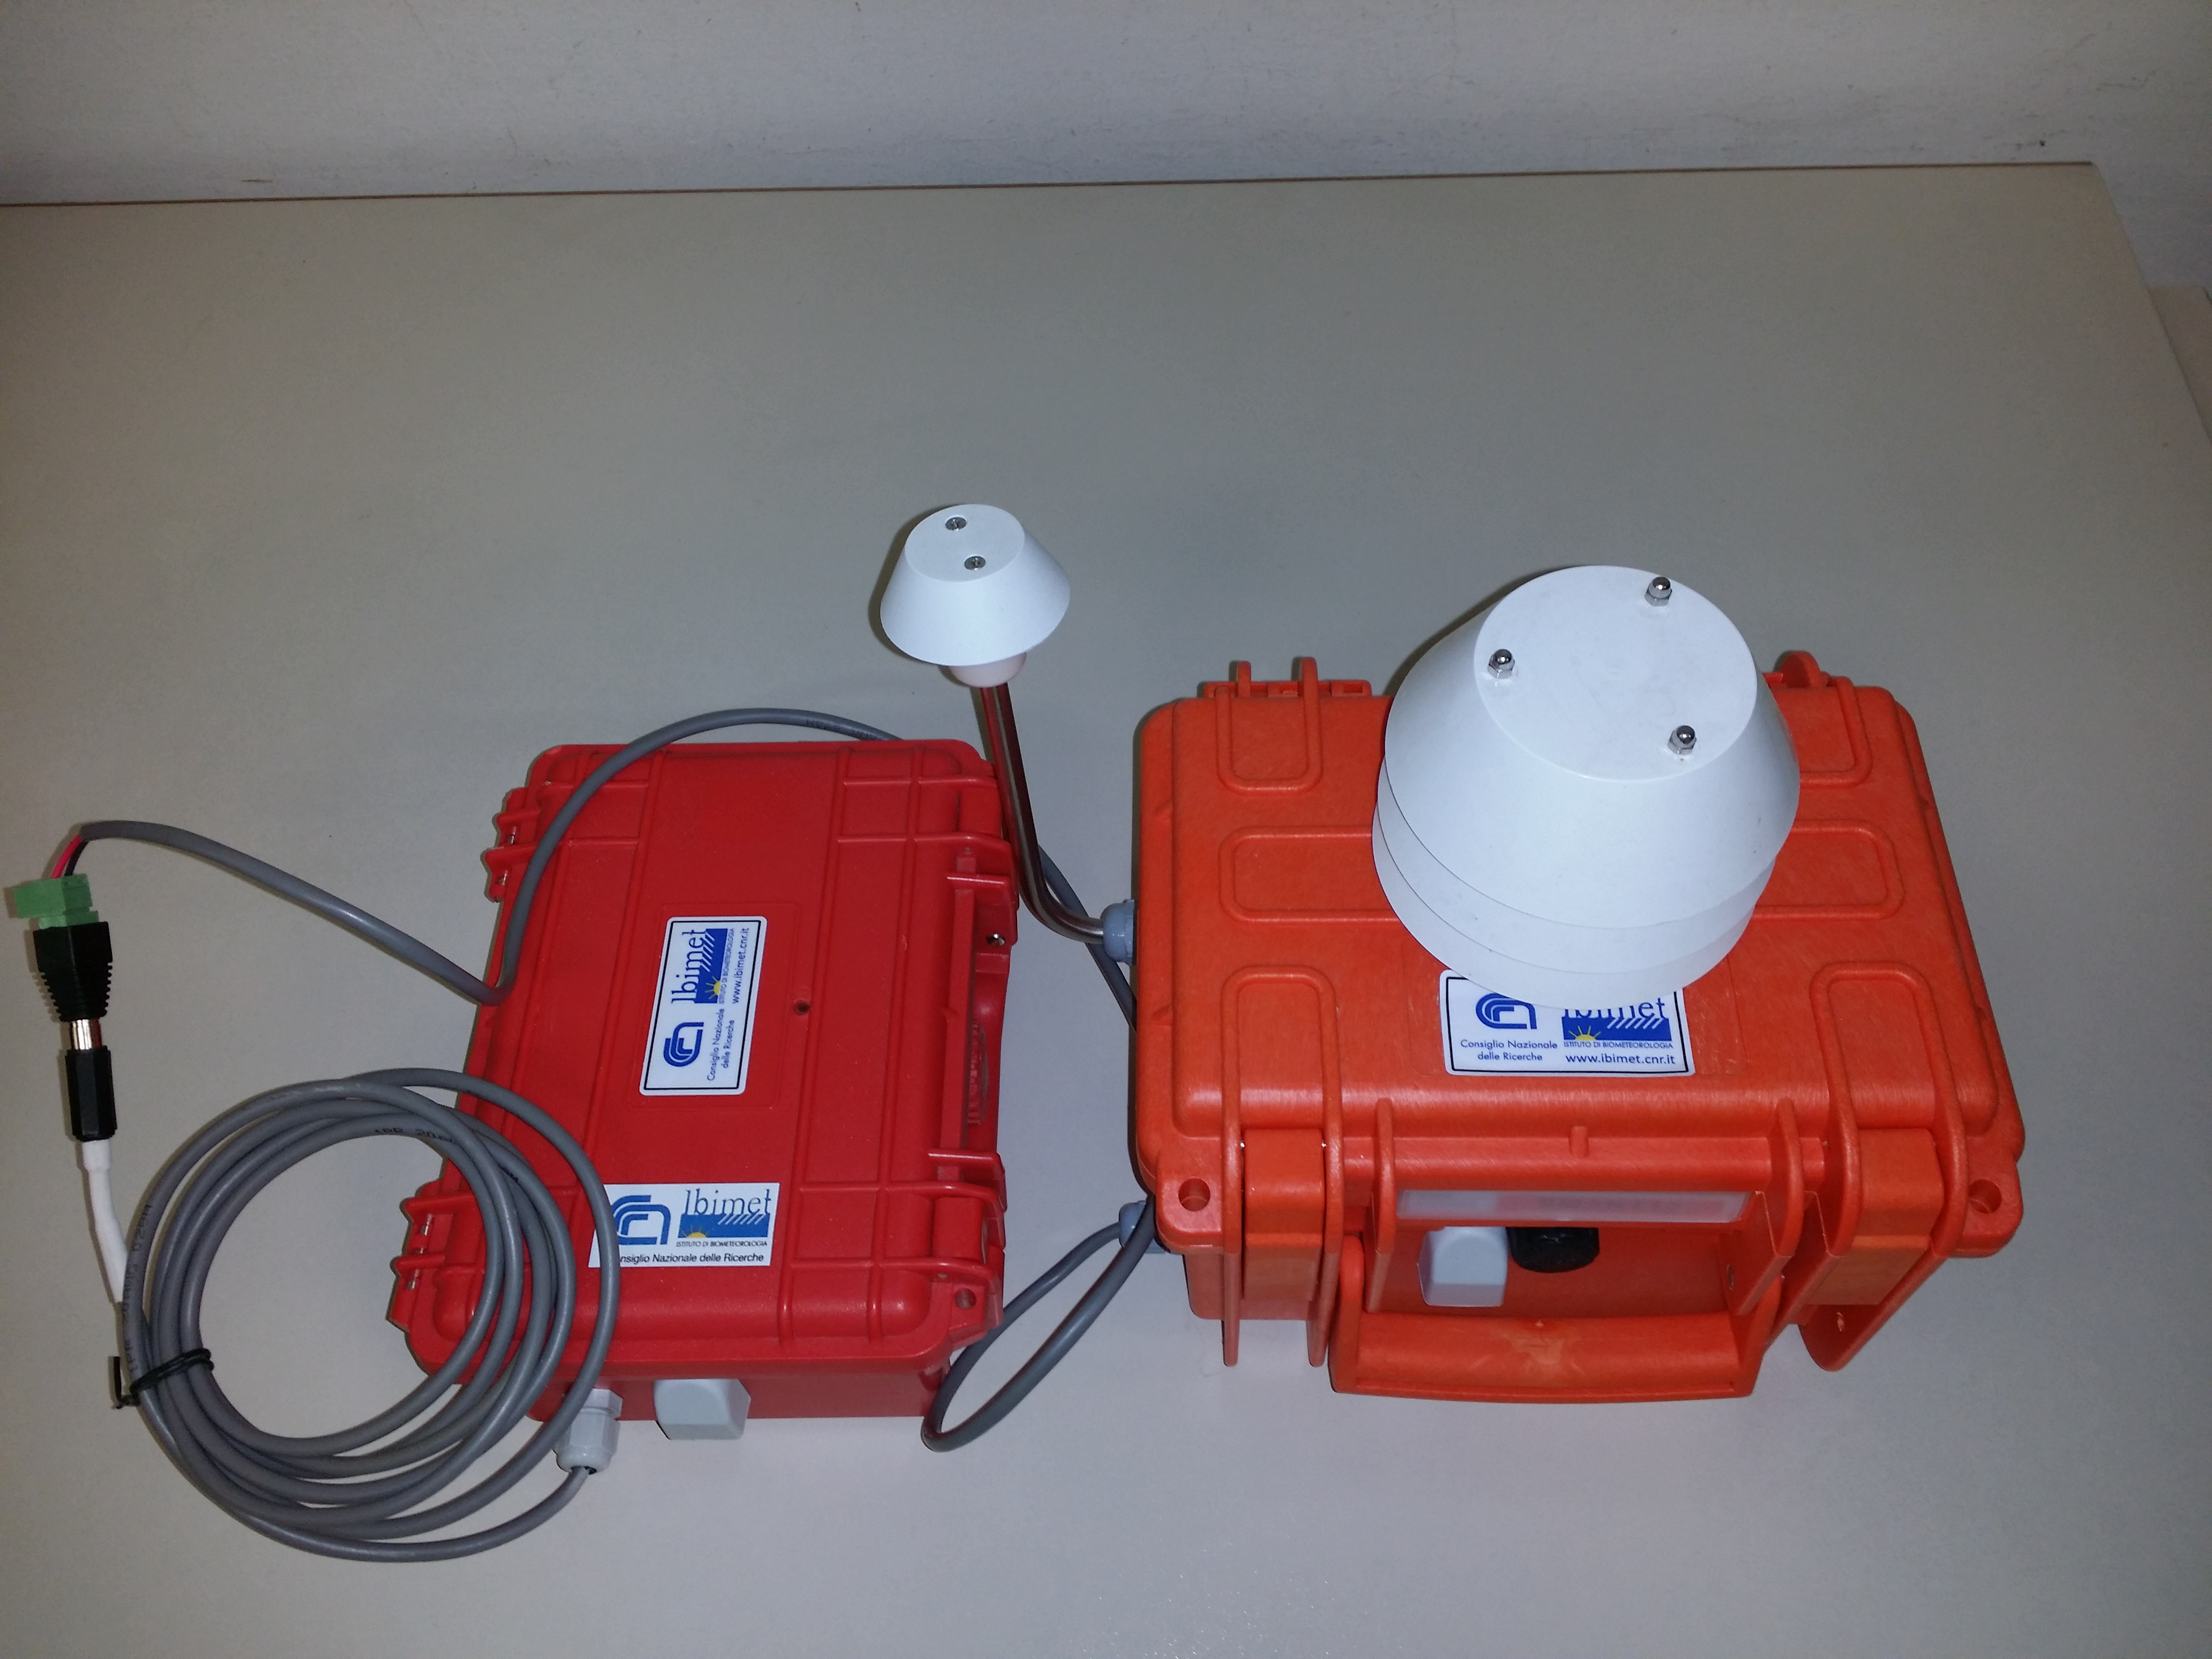
\includegraphics[width=.48\columnwidth]{figure/20171116_175931.jpg}
		\label{fig:nodes_tetra_3D}}
	\caption{IP68 box AirQino. The system is provided with an internal DC-DC converter unit that accepts a wide range of voltage inputs, from 10 V dc to 30 V dc.}
	\label{fig:ip68_image}
\end{figure} 
%%%%%%%%%%%%%%%%%%%%%%%%%%%%%%%%%%%%%%
    
The sensors installed on the board have a good accuracy, low cost as well as interfacing capabilities and they provide a good tradeoff between cost effectiveness and reliability to ensure the continuity and traceability of observations. The list of sensors with their specifications is reported in Table  \ref{tab:board_specifications}.
The measurement ranges of these sensors are reported in Table \ref{tab:board_range}.
%%%%%%%%%%%TABLE
\begin{table}[tbp]
 \centering
 \begin{center}  
  \begin{tabular}{c}
   % \begin{center}                                                                         
      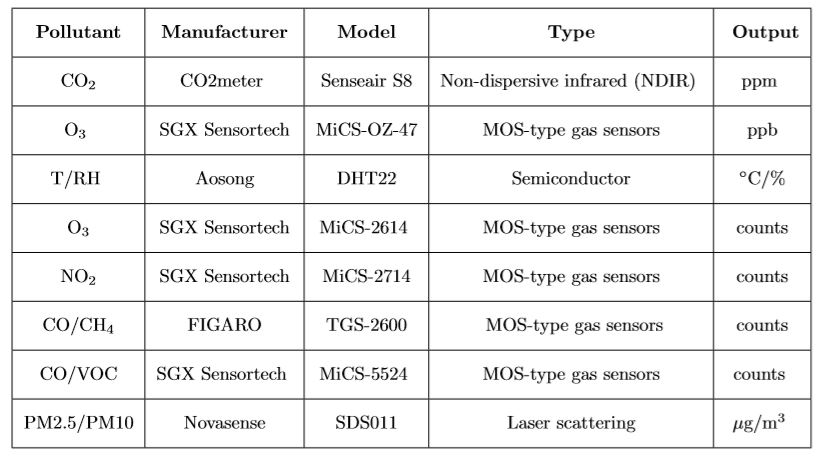
\includegraphics[width=0.45\textwidth]{figure/fig_sensor_spec.jpg} 
    %\end{center}     
  \end{tabular}
\end{center}  
\caption{AirQino sensor specifications. The count range 0-1024 is the digital to analog conversion board scale.}
  \label{tab:board_specifications}
\end{table}
%%%%%%%END TABLE
%%%%%%%%%%%TABLE
\begin{table}[tbp]
 \centering
 \begin{center}  
  \begin{tabular}{c}
   % \begin{center}                                                                         
      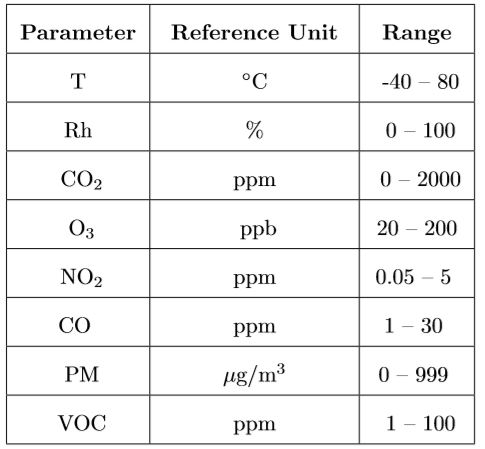
\includegraphics[width=0.4\textwidth]{figure/fig_sensor_range.jpg} 
    %\end{center}     
  \end{tabular}
\end{center}  
\caption{AirQino sensor ranges in reference unit measure.}
  \label{tab:board_range}
\end{table}


In addition to the IP68 box AirQino (see Figure \ref{fig:ip68_image}), two other versions have been used in the monitoring work:%;  
\begin{itemize}
\item \textit{Indoor AirQino}: used for indoor measurements (see Figure \ref{fig:arq_indoor}) as explained in Section \ref{sec:intro4} to allow the evaluation of a mean pollutant concentration within closed places (buildings) and estimate plausible initial condition values.
\item \textit{Mobile AirQino}: installed on a special bike (see Figure \ref{fig:arq_mobile}) developed by the Department of Industrial Engineering of the University of Florence (Italy). This station version includes a Bluetooth module. 
%%%%%%%%%%%%%%%%%%%%%%%%%%%%%
\end{itemize}
%%%%%%%%%%%%%%%%%%%%%%%%%%%
\begin{figure}[tbp]
	\centering
	\subfloat[]{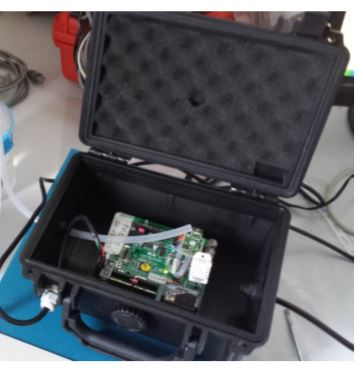
\includegraphics[width=.48\columnwidth]{figure/fig_sensor_indoor.jpg}
		\label{fig:arq_indoor}}
	\hfil
	\subfloat[]{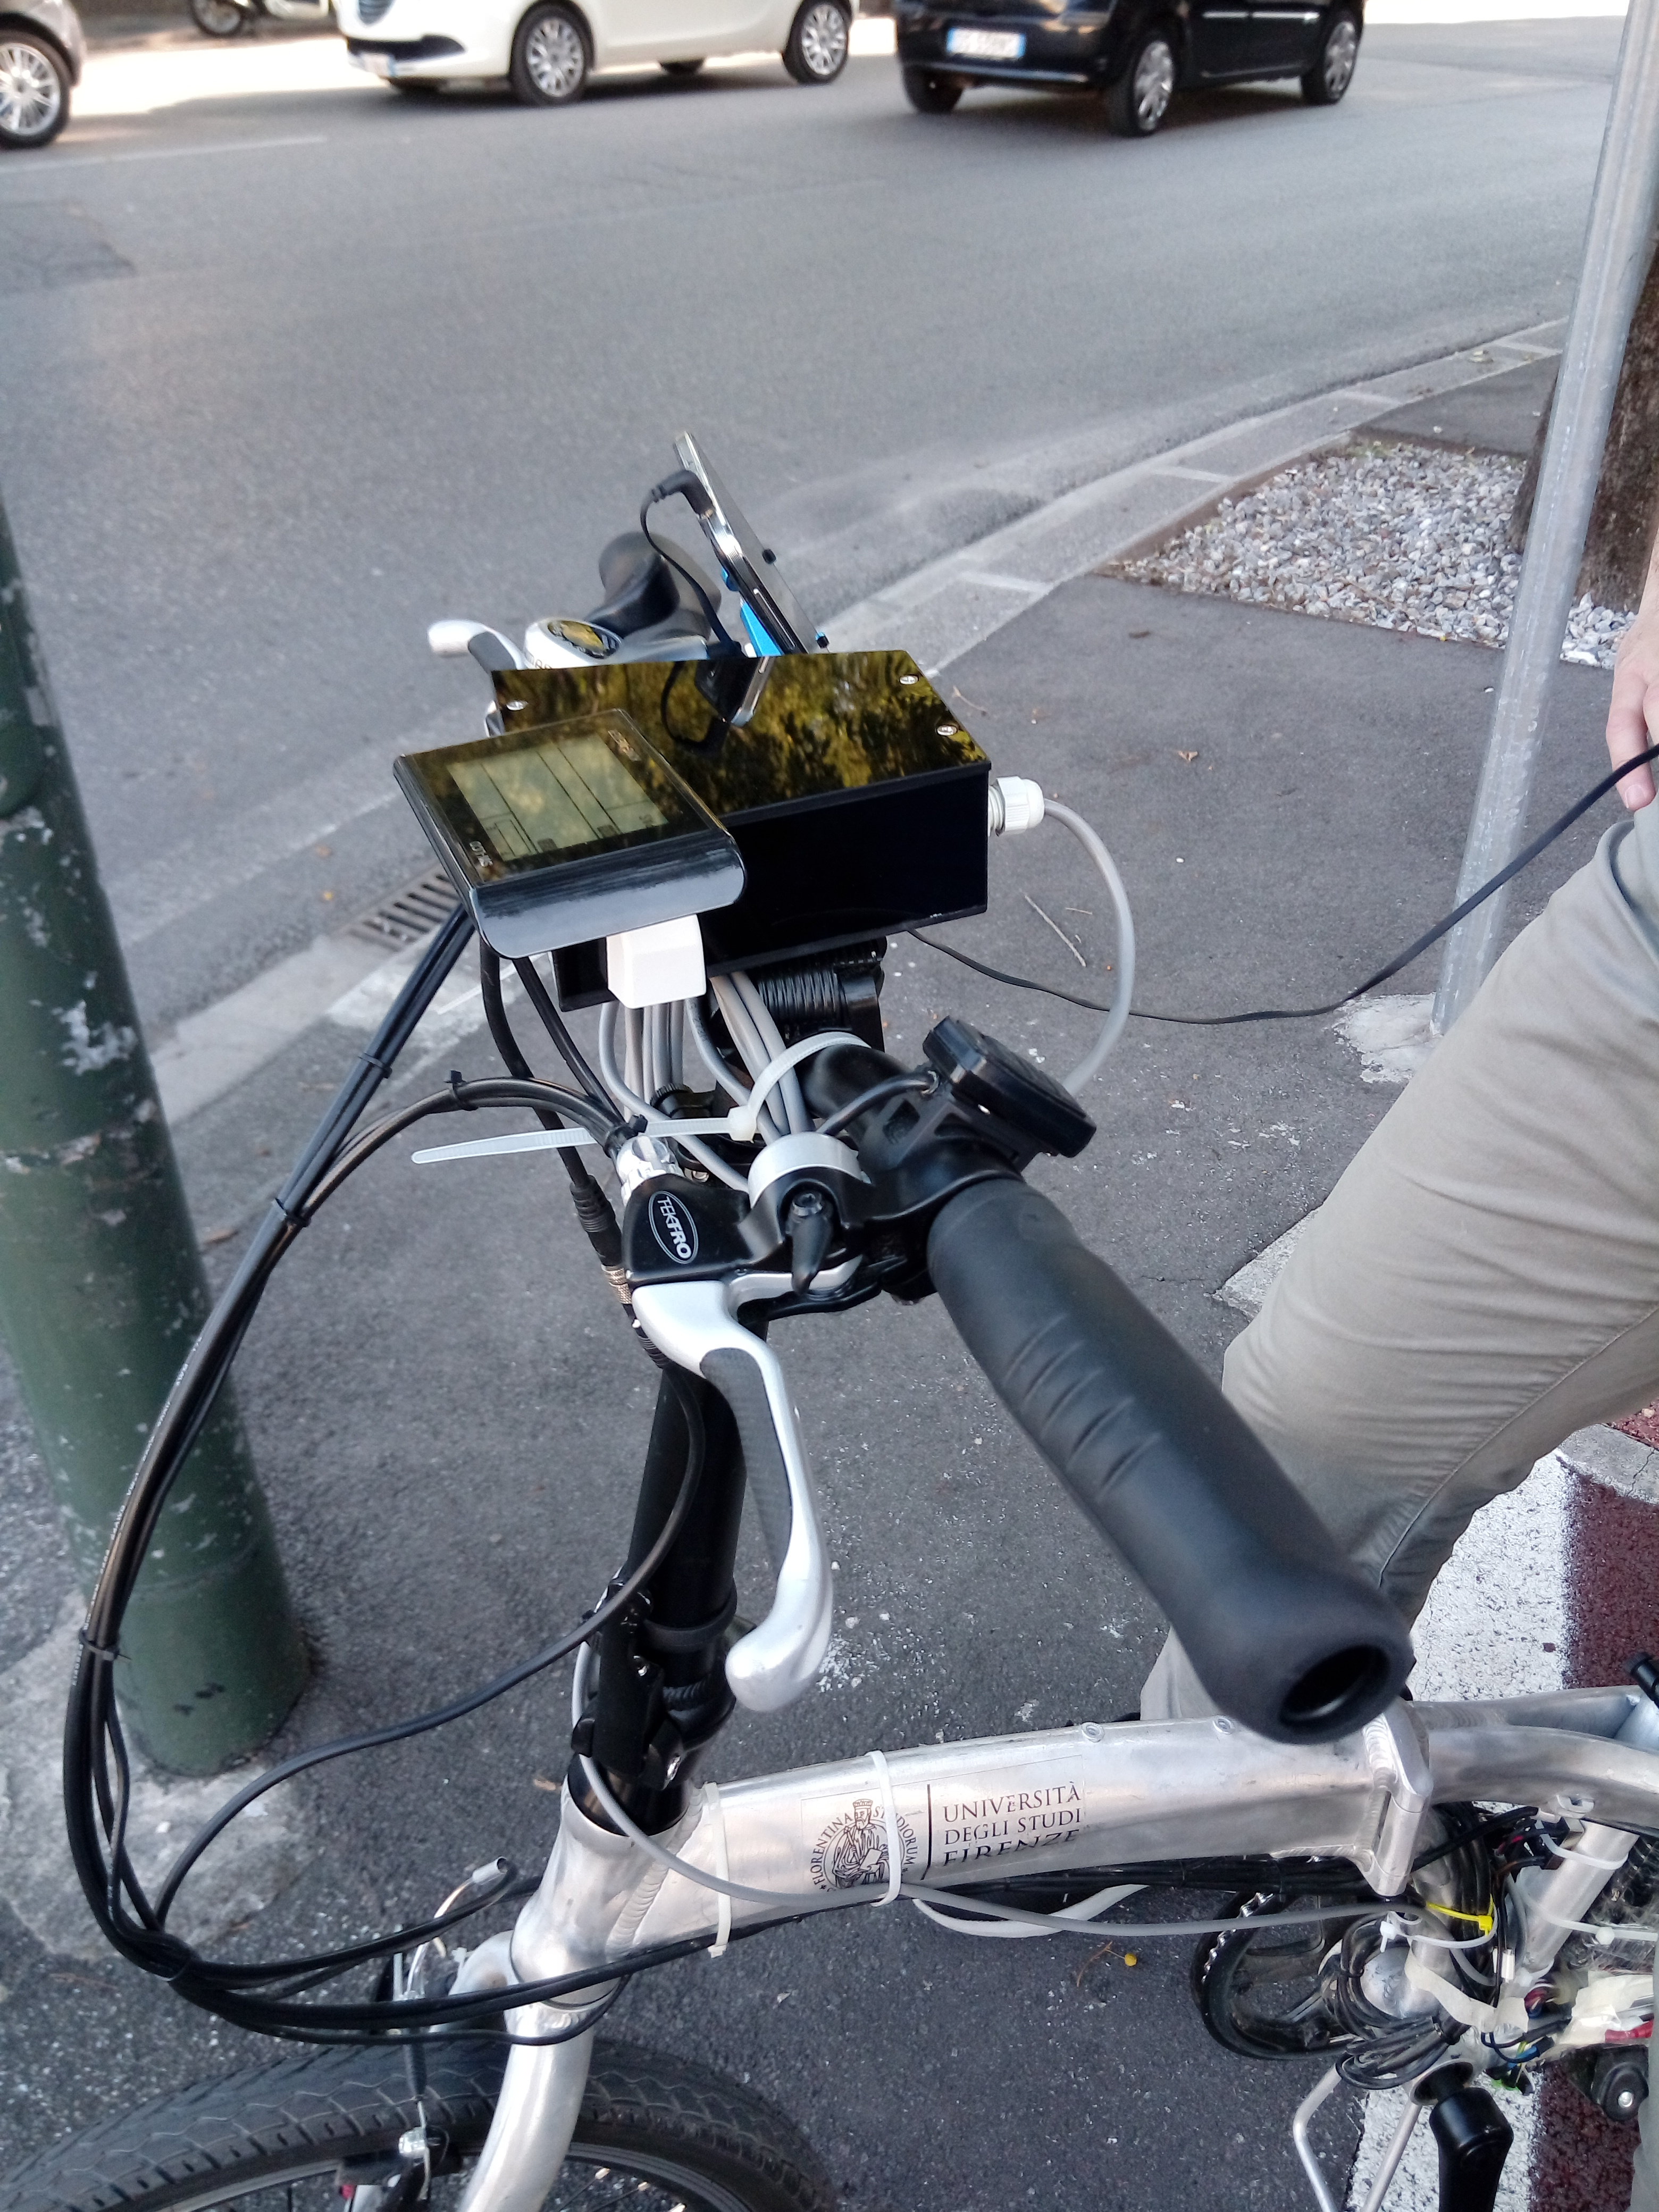
\includegraphics[width=.48\columnwidth]{figure/fig_sensor_bike_1.jpg}
		\label{fig:arq_mobile}}
	\caption{Indoor AirQino (a) and Mobile AirQino (b).}
	\label{fig:arq_ind_mobile}
\end{figure}
In both versions a Bluetooth module is included. To collect data, an Android phone application  is provided to manage, via Bluetooth, sensor reading and to track the cell phone GPS signal.


\section{Air-quality monitoring case-study}
The geographical area chosen for studying the behavior of pollutants is an urban cross-section of the city of Florence, in the Novoli area, limited to the north by \textit{Via di Novoli} and \textit{Via Maragliano}, to the south by \textit{Via Francesco Baracca} and \textit{Via del Ponte alle Mosse}, to the west by \textit{Via Niccol\`o Paganini} and to the east by \textit{Via Francesco Doni}, as shown in Figure \ref{fig:bound_sat}. This area has been chosen since it contains two fixed traffic pollution measurement terminals, one located in \textit{Via del Ponte alle Mosse} of ARPAT, and the other one in \textit{Via della Villa Demidoff} of IBIMET-CNR.
%figure
\begin{figure}[tb]
	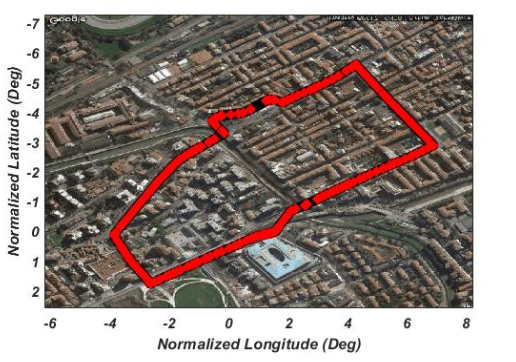
\includegraphics[width=0.5\textwidth]{figure/FinalBound3.png}
	\caption{Boundaries of the area of interest in Novoli, Florence, drawn on a \textit{Google Maps} satellite image.}
	\label{fig:bound_sat}
         % \end{center}
\end{figure}

%end figure

Using an online application known as \textit{geojson.io}  it has been possible to identify the geographic coordinates of the urban area of interest and import them into the Matlab environment to reconstruct the domain of the area and its geometry. The basic idea has been to subdivide the road network in subdomains about 20 [m] long, so as to allow a high-resolution and simulation capacity for the concentration of pollutants in the various road sections. Using the same method, it has also been possible to reconstruct the 2D-shape of the buildings and the intermediate areas between the road network and buildings, referred to as \textit{background}. The resulting geometry developed in the Matlab environment is shown in Figure \ref{fig:mesh_2}.
%figure
\begin{figure}[tbp]
	\centering
%\hspace*{-4cm}   
	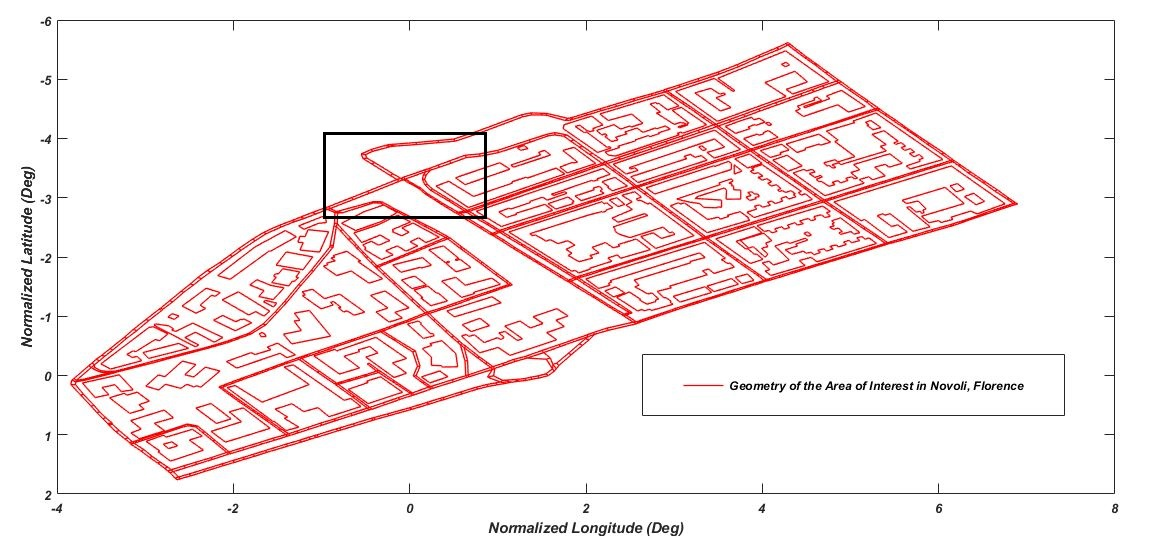
\includegraphics[width=.5\textwidth]{figure/Geometria_novoli_2.jpg}
	\caption{Geometry of the area of interest in Novoli, Florence, showing streets and buildings. The rectangle with the black border focuses on a cross-section of the geometry (Figure \ref{fig:spaccatogeom}), in which it can be seen how the streets have been divided into subsections.}
	\label{fig:mesh_2}
		\centering
\hspace*{-0.2cm}   
	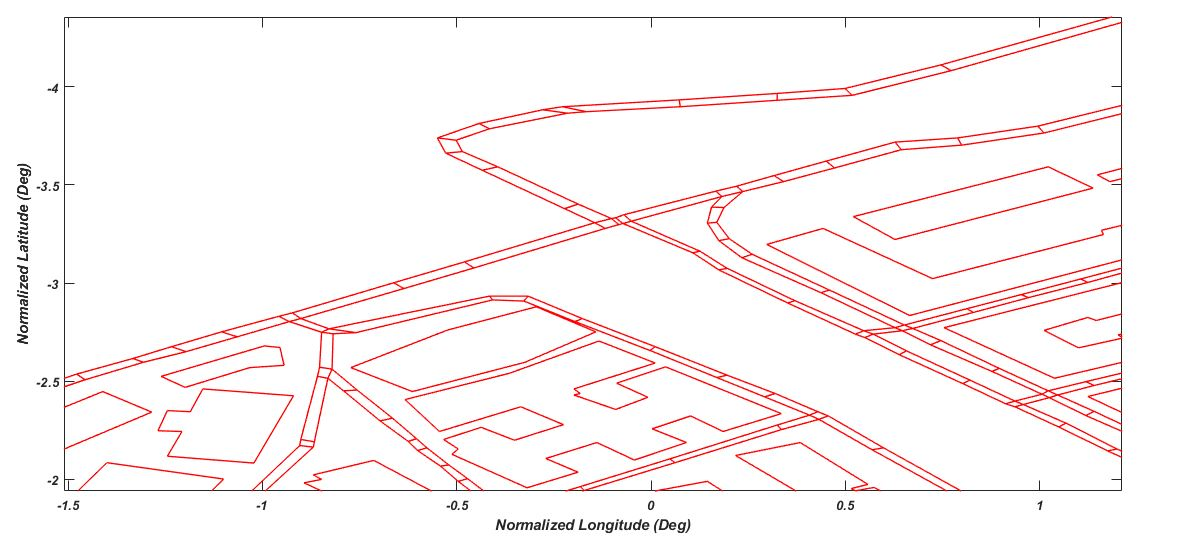
\includegraphics[width=.5\textwidth]{figure/spaccato_geo.jpg}
	\caption{Cross-section of the geometry of the area of interest. The subsections composing the urban roads are visible.}
	\label{fig:spaccatogeom}
         % \end{center}
\end{figure}
%\vspace{0.5mm}
%end figure
%figure

After generating the domain $\Omega$, it has been possible to generate the mesh with its relative elements via the \textit{Partial Differential Equation Toolbox\textsuperscript{TM}} (PDE Toolbox) which provides functions for solving partial differential equations in 2D, 3D, and time using finite element analysis. 
In Figure \ref{fig:geom_mesh}, the mesh nodes $\textbf{p}_{i}$ are clearly visible. The parameters concerning the complexity and space resolution of the adopted model for the considered Novoli area are reported in Table \ref{tab:Mesh_properties}.
\begin{table}[tbp]
\centering
 \begin{center}  
  \begin{tabular}{|c|c|}
\hline
Number of nodes & 28144 \\ \hline
Number of elements & 55453 \\ \hline
Number of edges & 12333 \\
\hline
  \end{tabular}
\end{center}  
\caption{Mesh properties.}
  \label{tab:Mesh_properties}
\end{table}
%Notice that resolving high system order $n =$ 28144 calls for the use of a computationally efficient variant of the Kalman filter, e.g. the ensemble Kalman filter presented in Chapter \ref{ch:DataAss}. 
\begin{figure}[tbp]
	\centering
\hspace*{0cm}%-2 .6   
	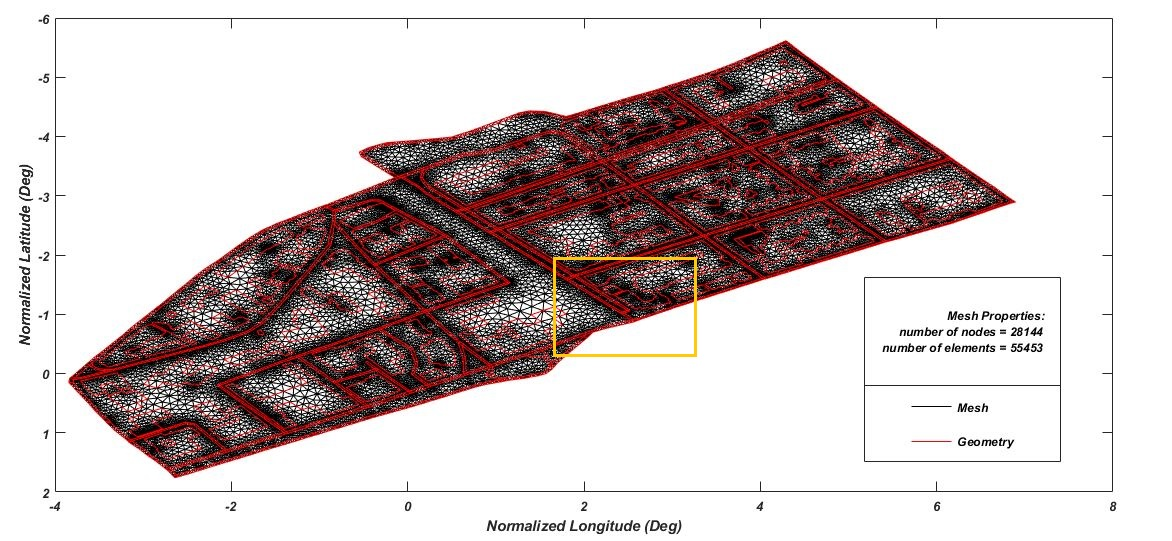
\includegraphics[width=.5\textwidth]{figure/Mesh_3.jpg}
	\caption{Mesh extrapolated from the geometry of the area of interest. At this magnification level, the elements of the mesh are almost indistinguishable; conversely the elements are visible at a higher magnification level as shown in Figure \ref{fig:geom_mesh_2}, where the mesh cross-section within the yellow-bordered box is enlarged.}
	\label{fig:geom_mesh}
		\centering
\hspace*{0cm}%-2 .6   
	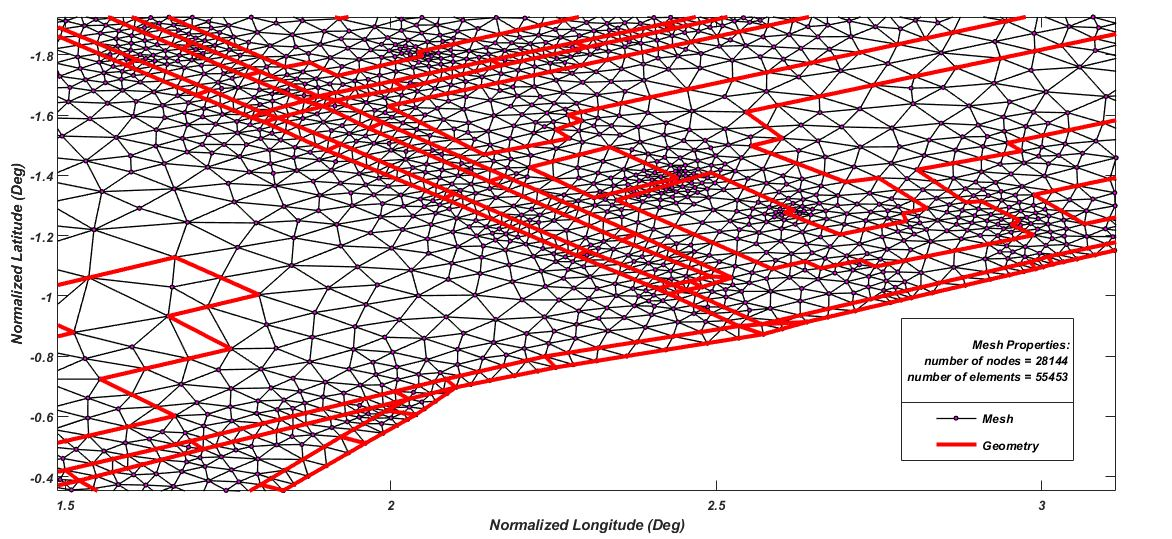
\includegraphics[width=.5\textwidth]{figure/cross_section_mesh.jpg}
	\caption{Cross-section of the mesh shown in Figure \ref{fig:geom_mesh}. At this magnification level the elements are clearly visible.}
	\label{fig:geom_mesh_2}
         % \end{center}
         % \end{center}
\end{figure}


\section{Simulation results}
In this section, we present the results of the EnKF-based data assimilation algorithm on synthetic data generated from a simulation scenario modeling the diffusion of  
CO$_2$ in the area of interest. 
The simulated scenario matches the first measurement campaign both in terms of environmental conditions (i.e. traffic flow, diffusivity, wind intensity and direction) 
and measurement collection (i.e., timing and geographical position of the measurements within the area of interest).
This choice makes it possible to evaluate, in a comprehensive way, the capability of the proposed data assimilation algorithm to estimate the concentration field in a realistic scenario
by considering the data generated by the simulator as \textit{ground truth} for the filter. The internal emissions used in filter 
are different from the one used in the simulator, and specifically are obtained from the latter by inserting a random noise. In this way, we can model the fact that, in practice, the true emissions can
only be known approximately.

Performance was evaluated by means of two criteria: the Space Averaged Root Mean Square Error (SA-RMSE) and the Time averaged RMSE (TA-RMSE).
The SA-RMSE for the state estimate $\hat{\mb{x}}_{k|k}$ at time instant $k$ calculated using $N_{P}$ Monte Carlo simulations is defined as
\begin{align} \label{eq:rmse_time}
SA\mbox{-}RMSE(k) \overset{\Delta}{=} \sqrt{\dfrac{1}{N_Pn}\sum_{i=1}^{N_P}\tilde{\mb{x}}_{k|k}^{\mathrm{T}}(i)\tilde{\mb{x}}_{k|k}(i)}
\end{align}
where $\tilde{\mb{x}}_{k|k}(i) = \mb{x}_{k} - \hat{\mb{x}}_{k|k}(i)$  is the estimate error and $\hat{\mb{x}}_{k|k}(i)$ is the estimate of $\mb{x}_{k}$ relative to the $i$-th Monte Carlo trial. 
The TA-RMSE is instead defined as 
\begin{align} \label{eq:rmse_space}
TA\mbox{-}RMSE(j) \overset{\Delta}{=} \sqrt{\dfrac{1}{N_PN_T}\sum_{i=1}^{N_P} \sum_{k=1}^{N_T}(\tilde{x}_{k|k,j})^2}, \ \text{for } j=1,\dots,n% \mbox{in} \ \Omega
\end{align}
where $n$ is the total number of the mesh nodes, $N_T$ is the total number of time steps, $\tilde{x}_{k|k,j} = {x}_{k,j} - \hat{x}_{k|k,j}$ and $\hat{x}_{k|k,j}$ is the pollutant concentration estimate of $\mb{x}_{k}$ in the $j-$th node of the mesh at time instant $k$.
Notice that the SA-RMSE allows one to evaluate how the estimation error varies with time, also as a function of the collected measurements, whereas the TA-RMSE makes it possible
to evaluate the uniformity of the estimation error in the domain of interest.
Three different tests have been performed by considering an ensemble size of 10, 20, and 50, respectively. In each setting, the SA-RMSE and the TA-RMSE have been computed over 50 Monte Carlo
Trials.
From the examination of the obtained results, the following general conclusions can be drawn:
\begin{itemize}
\item The SA-RMSE decreases with the increase of the ensemble size $q$ as evident from Fig. \ref{fig:monte_tot_time}. As expected, in the time interval in which no measurement is collected
and, hence, only prediction is performed, the estimation error increases with time. However, as soon as new measurements arrive, the estimation error promptly decreases. This shows the
capability of the proposed algorithm to exploit data assimilation in order to correct the error of the model used in the prediction step.
\item The TA-RMSE is uniform all over the domain $\Omega$ (see Fig. \ref{fig:rmse_total_evaluation}), except on the boundary where such value is null because the CO$_2$ concentration is considered to be known
and used as boundary condition for both the simulator and the filter. This shows the capability of the proposed algorithm to correctly estimate the concentration field even where no measurement is collected
(recall that the measurement sampling points are depicted in Fig. \ref{fig:coordsensorinmap}). Notice that, also in this case, the error decreases as the ensemble size increases.
\end{itemize}
%%%%%%%%%%%%%%%%%%%%%%%%%%%%%%%%%%%%%%%%%%%%%
\begin{figure}[tbp] 
\hspace*{-1cm} 
	\centering
	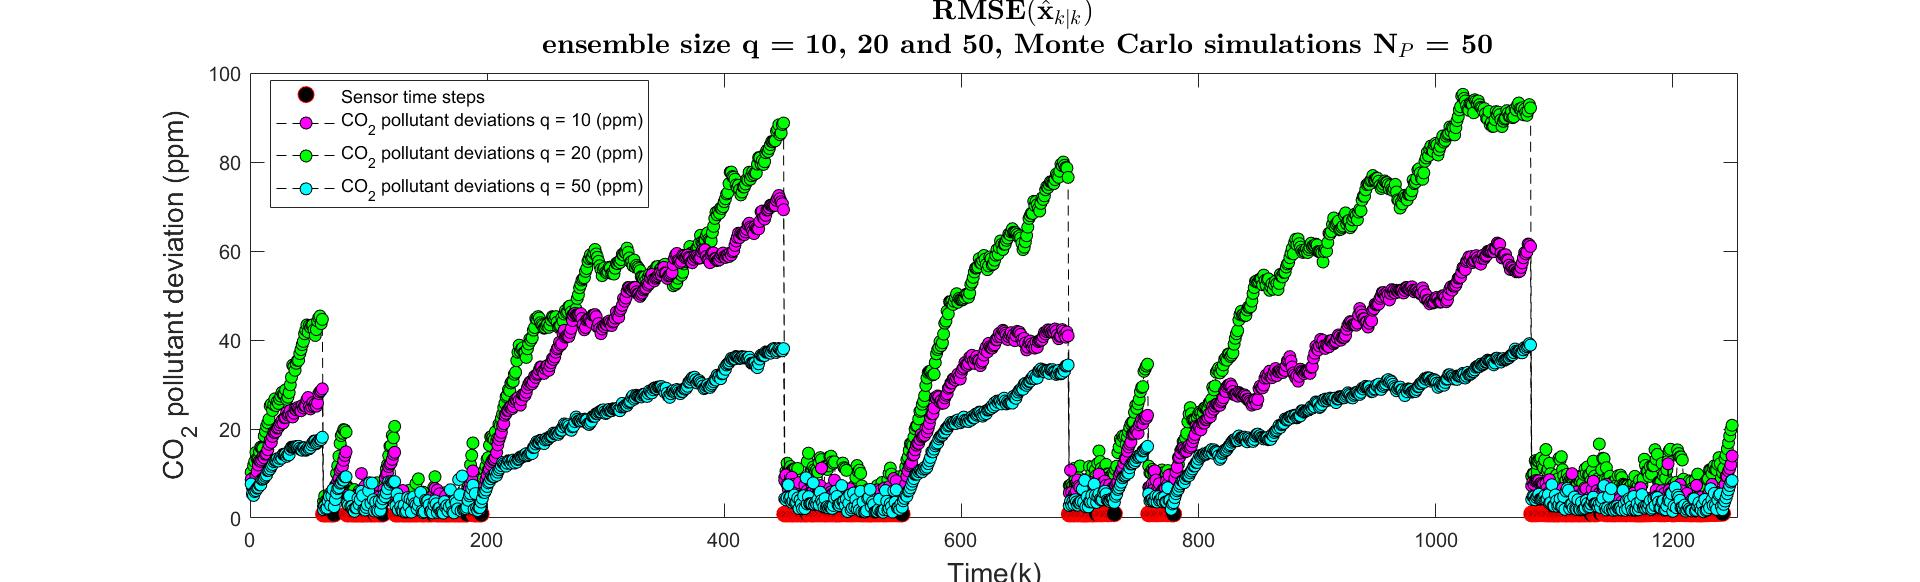
\includegraphics[width=1.2\columnwidth]{figure/monte_tot_ensemble_2.jpg}
	\caption{Performance evaluation on simulated data: time behavior of the SA-RMSE computed over 50 Monte Carlo trials considering three different ensemble sizes. 
	The red points on the abscissas represent the time instants in which a computer-simulated measurement is generated and used by the filter so as to update the estimate.}
		\label{fig:monte_tot_time}
\end{figure}


\begin{figure}[tbp]\ContinuedFloat
	\centering
	\subfloat[]{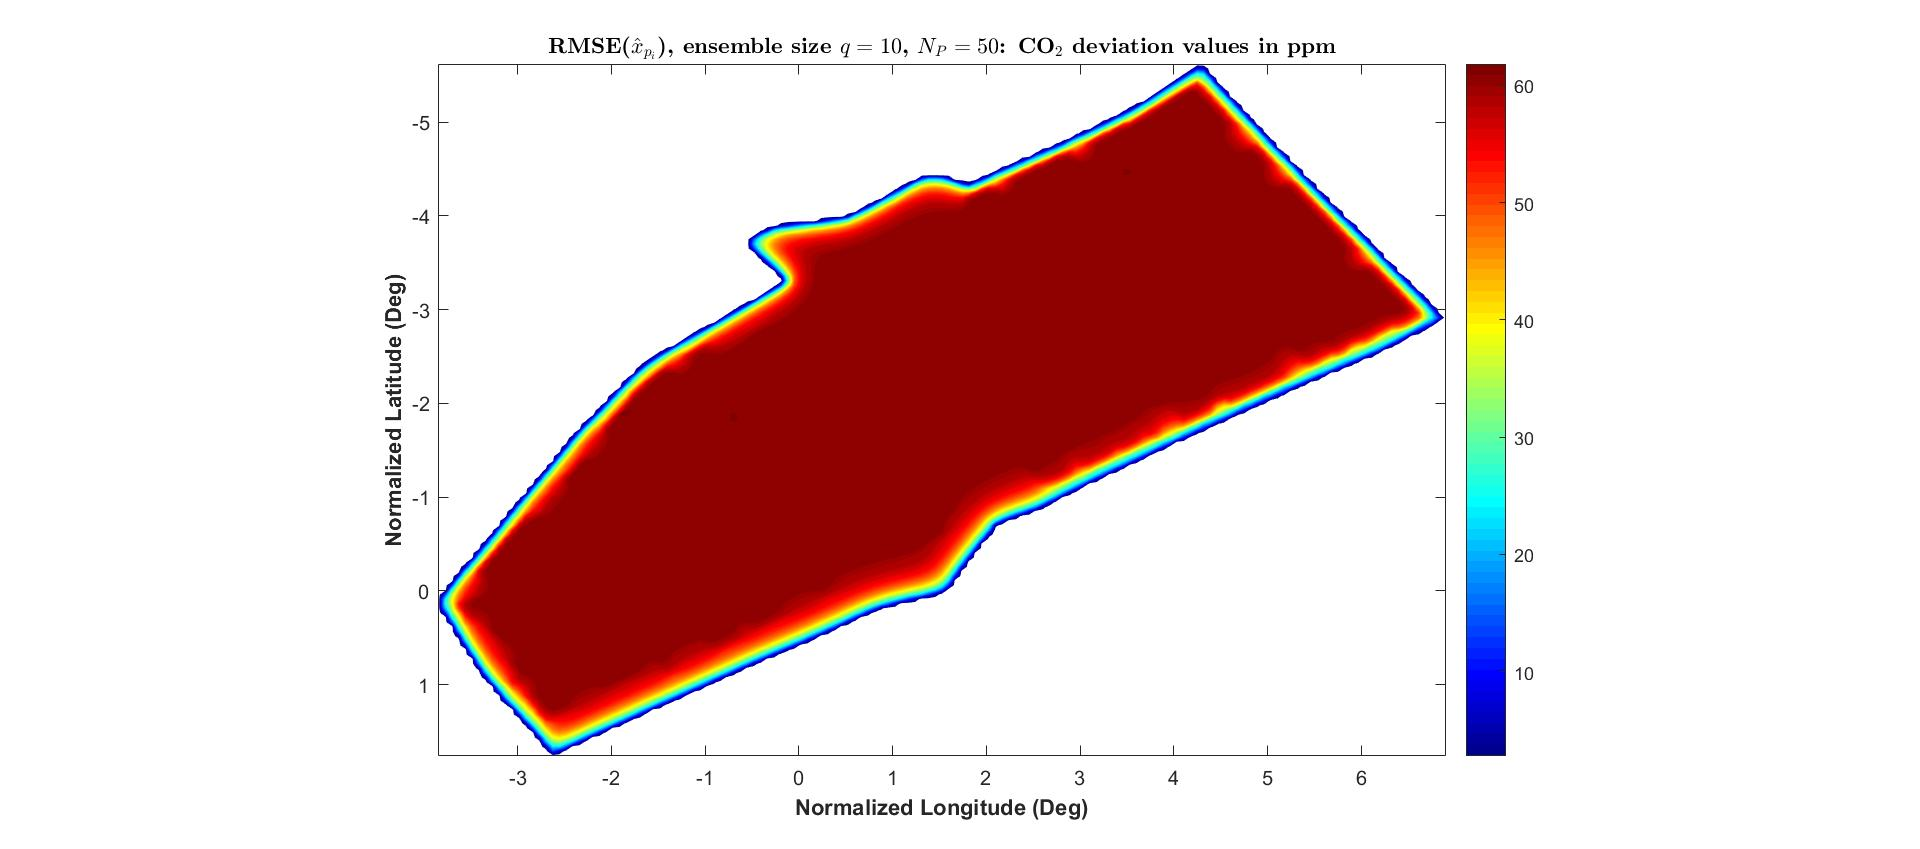
\includegraphics[width=1\columnwidth]{figure/monte_rmse_space_q10_2.jpg}}
	
	\subfloat[]{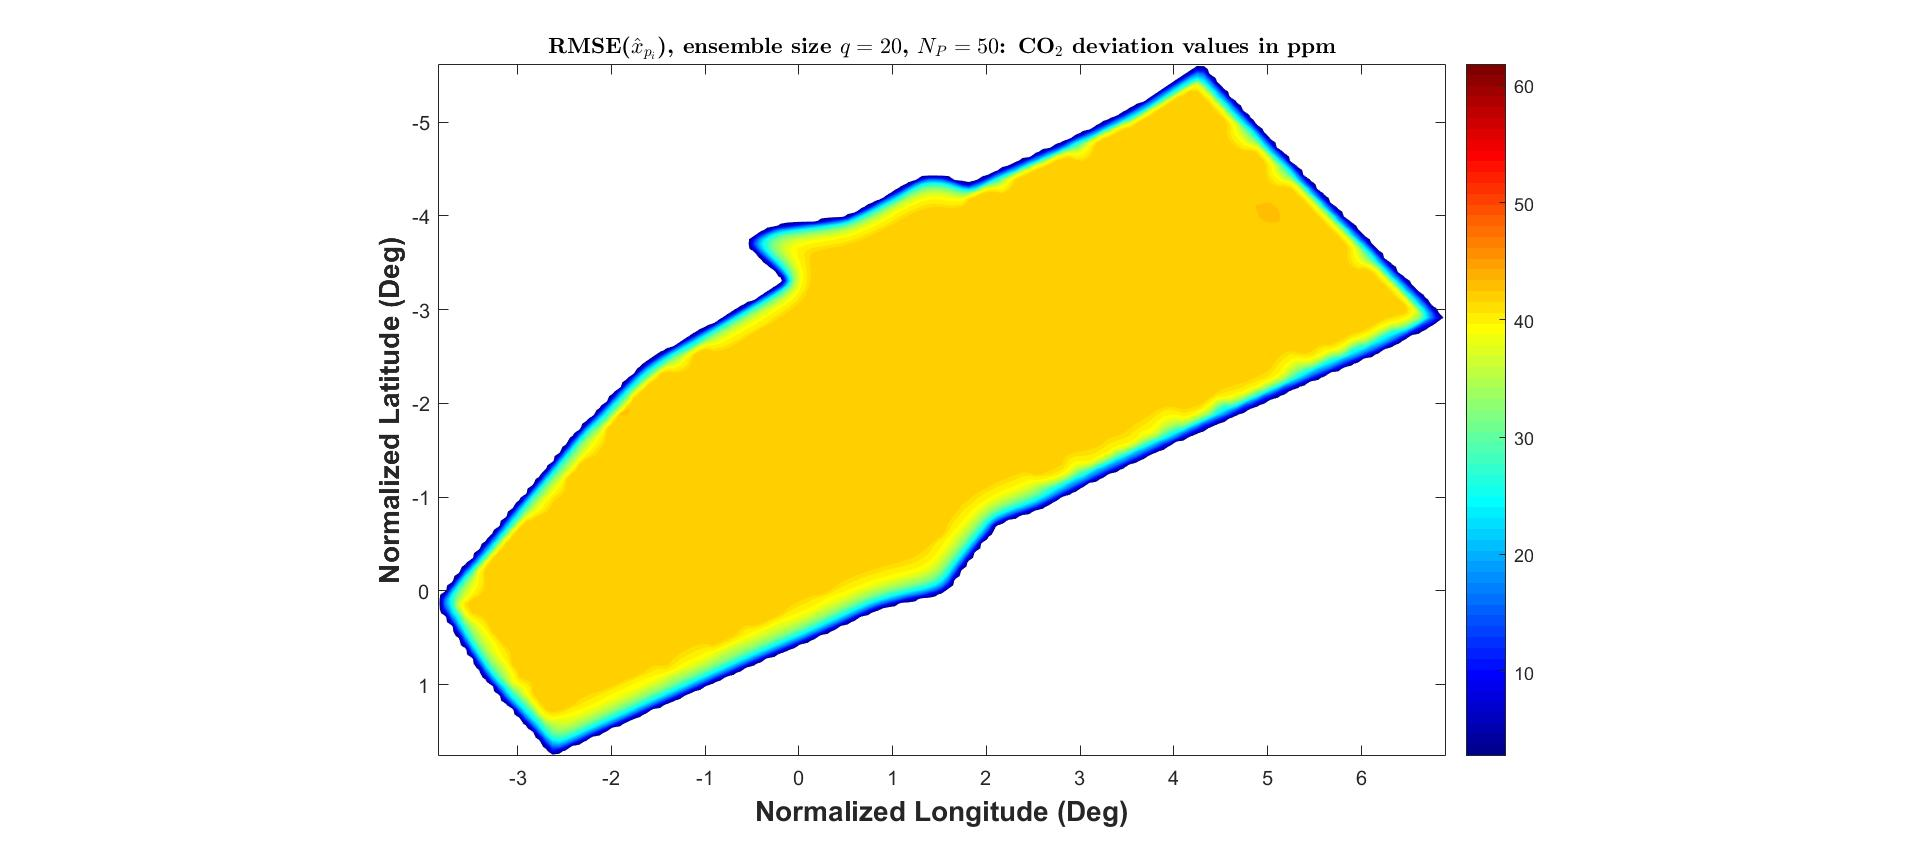
\includegraphics[width=1\columnwidth]{figure/monte_rmse_space_q20_2.jpg}}
	
	\subfloat[]{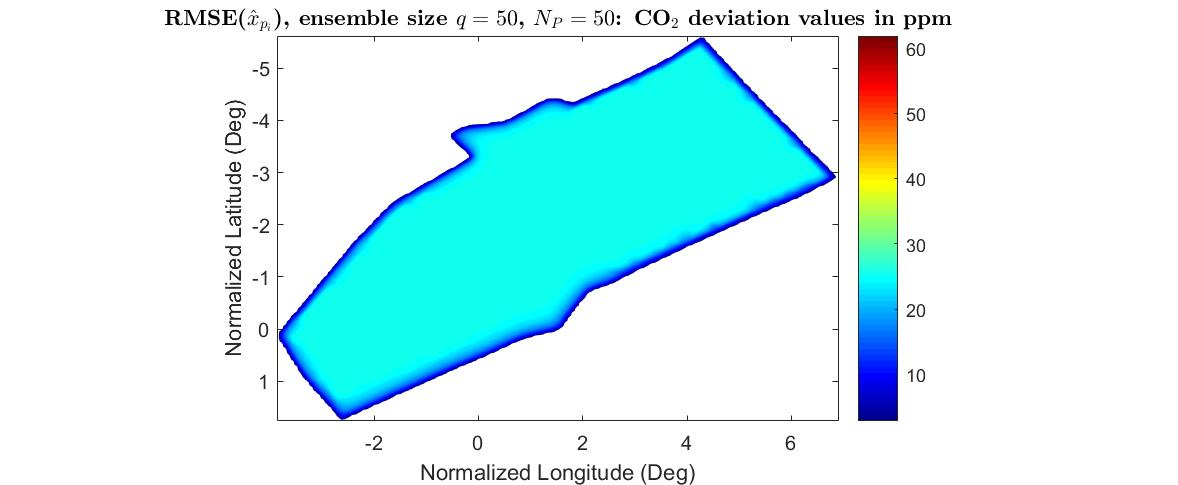
\includegraphics[width=1\columnwidth]{figure/monte_rmse_space_q50_2.jpg}}
\caption{Performance evaluation on simulated data: space distribution of the TA-RMSE computed over 50 Monte Carlo trials considering an ensemble size of 10 (a), 20 (b), and 50 (c), respectively.} \label{fig:rmse_total_evaluation}
\end{figure}

Since both the SA-RMSE and the TA-RMSE cannot be computed for experimental data (being the true concentration field unknown), it is  important to consider different evaluation criteria that
can be computed without using the true fields and, hence, can be used also for experimental data. For this purpose, one can resort either to regression functions
(see Fig. \ref{fig:regression_q150_monte}) or to quantitive criteria comparing the measurements (in this case the computer simulated pollutant concentration sample data) with the predicted observations.
Specifically, we have considered the Prediction RMSE (P-RMSE)
\begin{align} \label{eq:rmse_meas_4_4}
P\mbox{-}RMSE(k) \overset{\Delta}{=} \sqrt{\dfrac{1}{|\mathcal{S}_k|}(\hat{\mb{y}}_{k|k-1}-\mb{y}_k)^{\mathrm{T}}(\hat{\mb{y}}_{k|k-1}-\mb{y}_k)}, \ k \in \mathcal{K},
\end{align}
where $\mathcal{K} \subset \mathbb{R}$ is the set of sampling times and $\mathcal{S}_k$ is the set of coordinate points within the domain $\Omega$ wherein a measurement is collected at time $k$.
The time behavior of the P-RMSE is shown in Fig. \ref{fig:rmse_pred_error_q150monte}. The simulation parameters are shown in Table \ref{tab:Parameter_simulation_q150}, where $\sigma_{q}$ is the process noise standard deviation, i.e. $Q = \mb{I} \hspace{0.5mm} \sigma_{q}^{2}$ for all $k$. The results provided in Figs. \ref{fig:rmse_pred_error_q150monte} and \ref{fig:regression_q150_monte} confirm the effectiveness of the proposed data assimilation algorithm,



\begin{table}[tbp]
 \centering
 \begin{center}  
  \begin{tabular}{|c|c|c|c|c|}
\hline
  $N_T$ & $|\mathcal{K}|$ & $\sigma_{q}^{2}$ & $R_k$ & $\Delta$ \\  \hline
 1250 & 422 & $25^2$ & $3^2$ & $10$ \\
\hline
  \end{tabular}
\end{center}  
\caption{Performance evaluation on simulated data: simulation parameters.}
  \label{tab:Parameter_simulation_q150}
\end{table}
%%%%%%%END TABLE

%%%%%%%%%%end figure%%%%%%%%%%%%%%%%
%%%%%%figure%%%%
\begin{figure}[tbp]
		\hspace{-10mm}   
	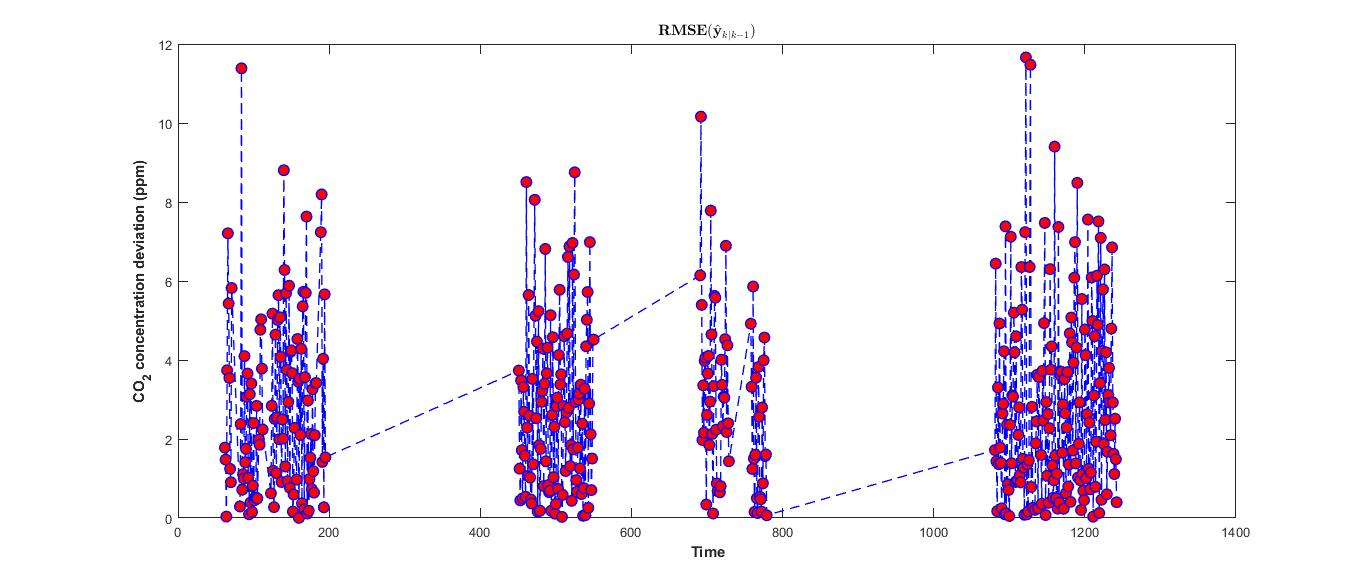
\includegraphics[scale=.22]{figure/montecarlo_q150_np1_error_2.jpg}
	\caption{Performance evaluation on simulated data: time behavior of the P-RMSE between the simulated CO$_2$ concentration values and the predictions of the data assimilation algorithm.
	In this simulation, the ensemble size was chosen equal to $150$.}
	\label{fig:rmse_pred_error_q150monte}
         % \end{center}
\end{figure}
%%%%%%%%%%end figure%%%%%%%%%%%%%%%%
%%%%%%%%%%%%%%%%%%%%%%%%%%%%%%%%%%%%%%%%%%%%%
\begin{figure}[tbp]
\hspace*{-1cm} 
	\centering
	\subfloat[]{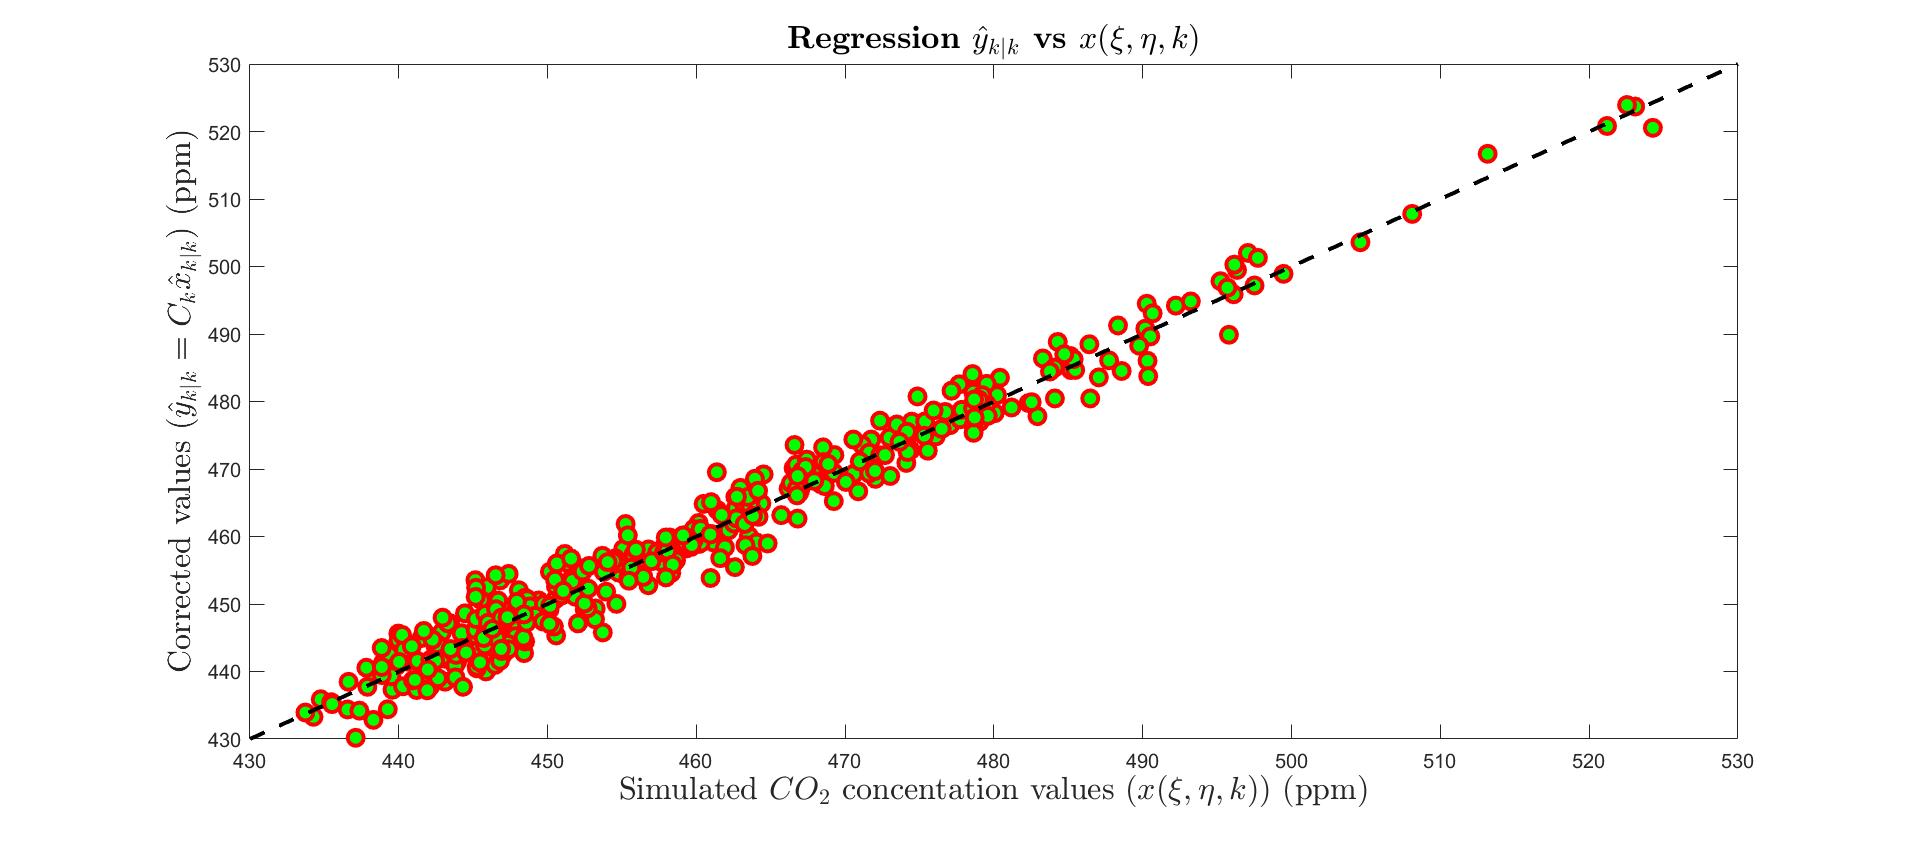
\includegraphics[width=1.2\columnwidth]{figure/montecarlo_q150_np1_corr_regression_2.jpg}
		\label{fig:regression_q150_monte_a}}
	\hfil
\hspace*{-1cm} 
	\subfloat[]{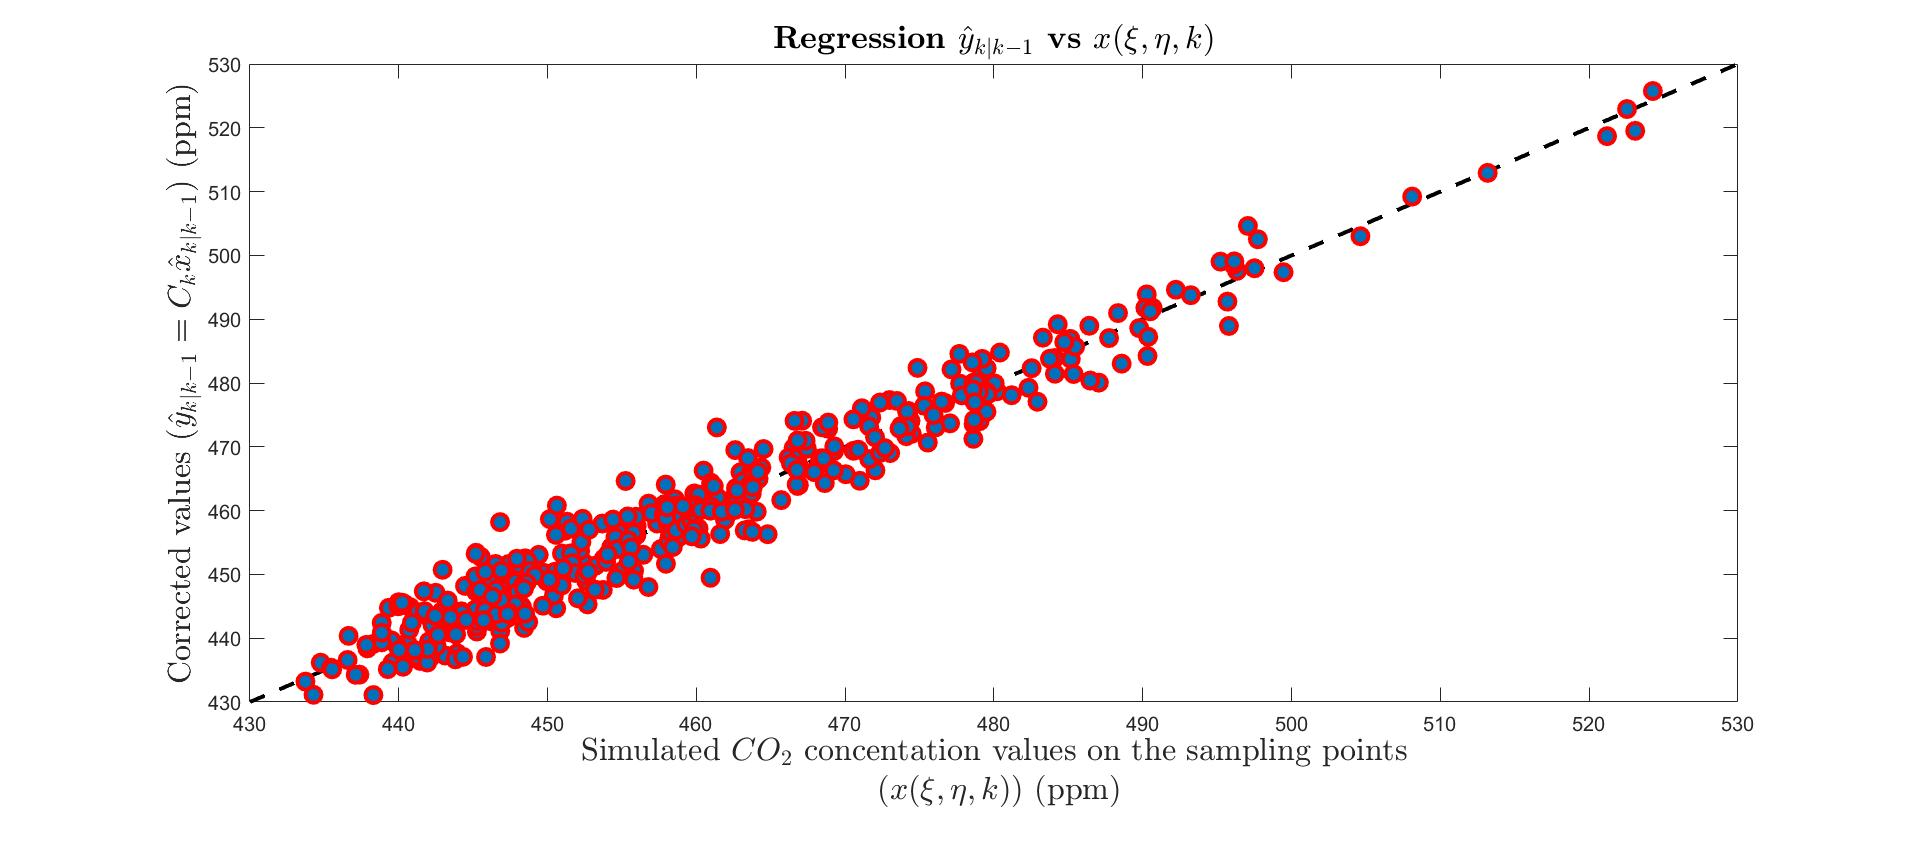
\includegraphics[width=1.2\columnwidth]{figure/montecarlo_q150_np1_pred_regression_new_2.jpg}
		\label{fig:regression_q150_monte_b}}
	\caption{Performance evaluation on simulated data:  regression functions comparing simulated computer CO$_2$ concentration values and both the corresponding corrections $\hat{y}_{k|k}$, $k \in \mathcal{K}$ (a) and predictions $\hat{y}_{k|k-1}$, $k \in \mathcal{K}$ (b).}
	\label{fig:regression_q150_monte}
\end{figure}


We conclude the perform evaluation on the simulata data by comparing the CO$_2$ concentration field of the simulated model with the estimated field obtained by means of the proposed
data assimilation algorithm. Three frames corresponding to three different time instants have been selected and displayed in Figure \ref{fig:sim_fil_comparison}. The big black spot shown into the domain of interest on the estimated field representation is the sampling point of the computer simulated measurement at the considered time instant.  From the examination of the obtained results, the following general conclusions can be drawn:
\begin{itemize}
\item the estimated field is very close to the simulated one (i.e., the ground truth), hence confirming the effectiveness of the considered data assimilation algorithm;
\item the mean CO$_2$ concentration increases over time because of the increasing emission level due to the traffic flow data collected from the \textit{ArcGis} websource (see Section \ref{sec:intro4}). 
In fact, the considered time slot  coincides with an increase in the level of traffic within the considered urban area; 
\item Figure \ref{fig:sim_fil_comparison} shows how the average concentration along the roads is greater than in the background or in buildings where the diffusion coefficient is lower. Furthermore, the CO$_2$ concentration in the streets is consistent with the traffic flow data collected from the \textit{ArcGis} web platform.
\end{itemize}




\begin{figure}[tbp]
	\centering
	\subfloat[]{ 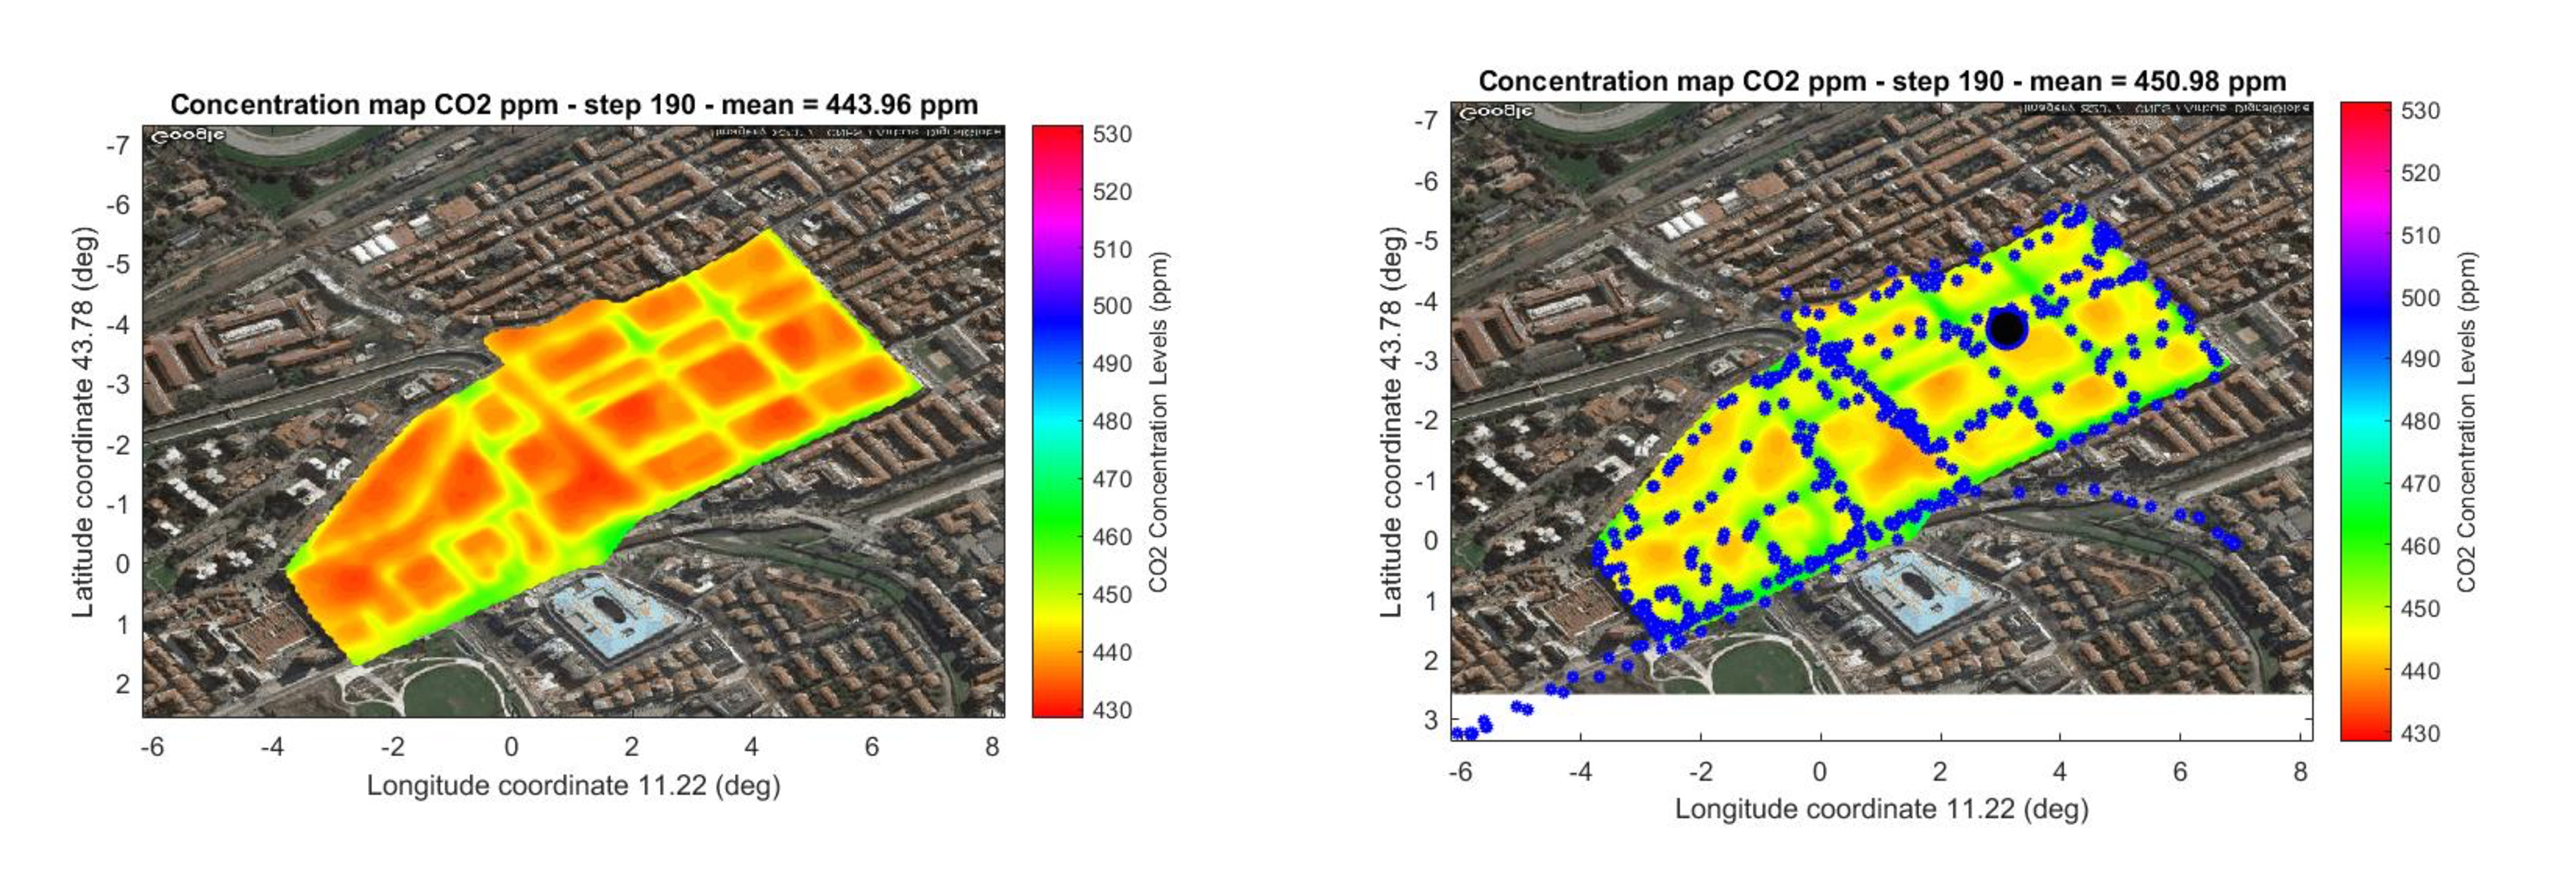
\includegraphics[width=1\columnwidth]{figure/step190}}
	
	\subfloat[]{\hspace{0.05cm} 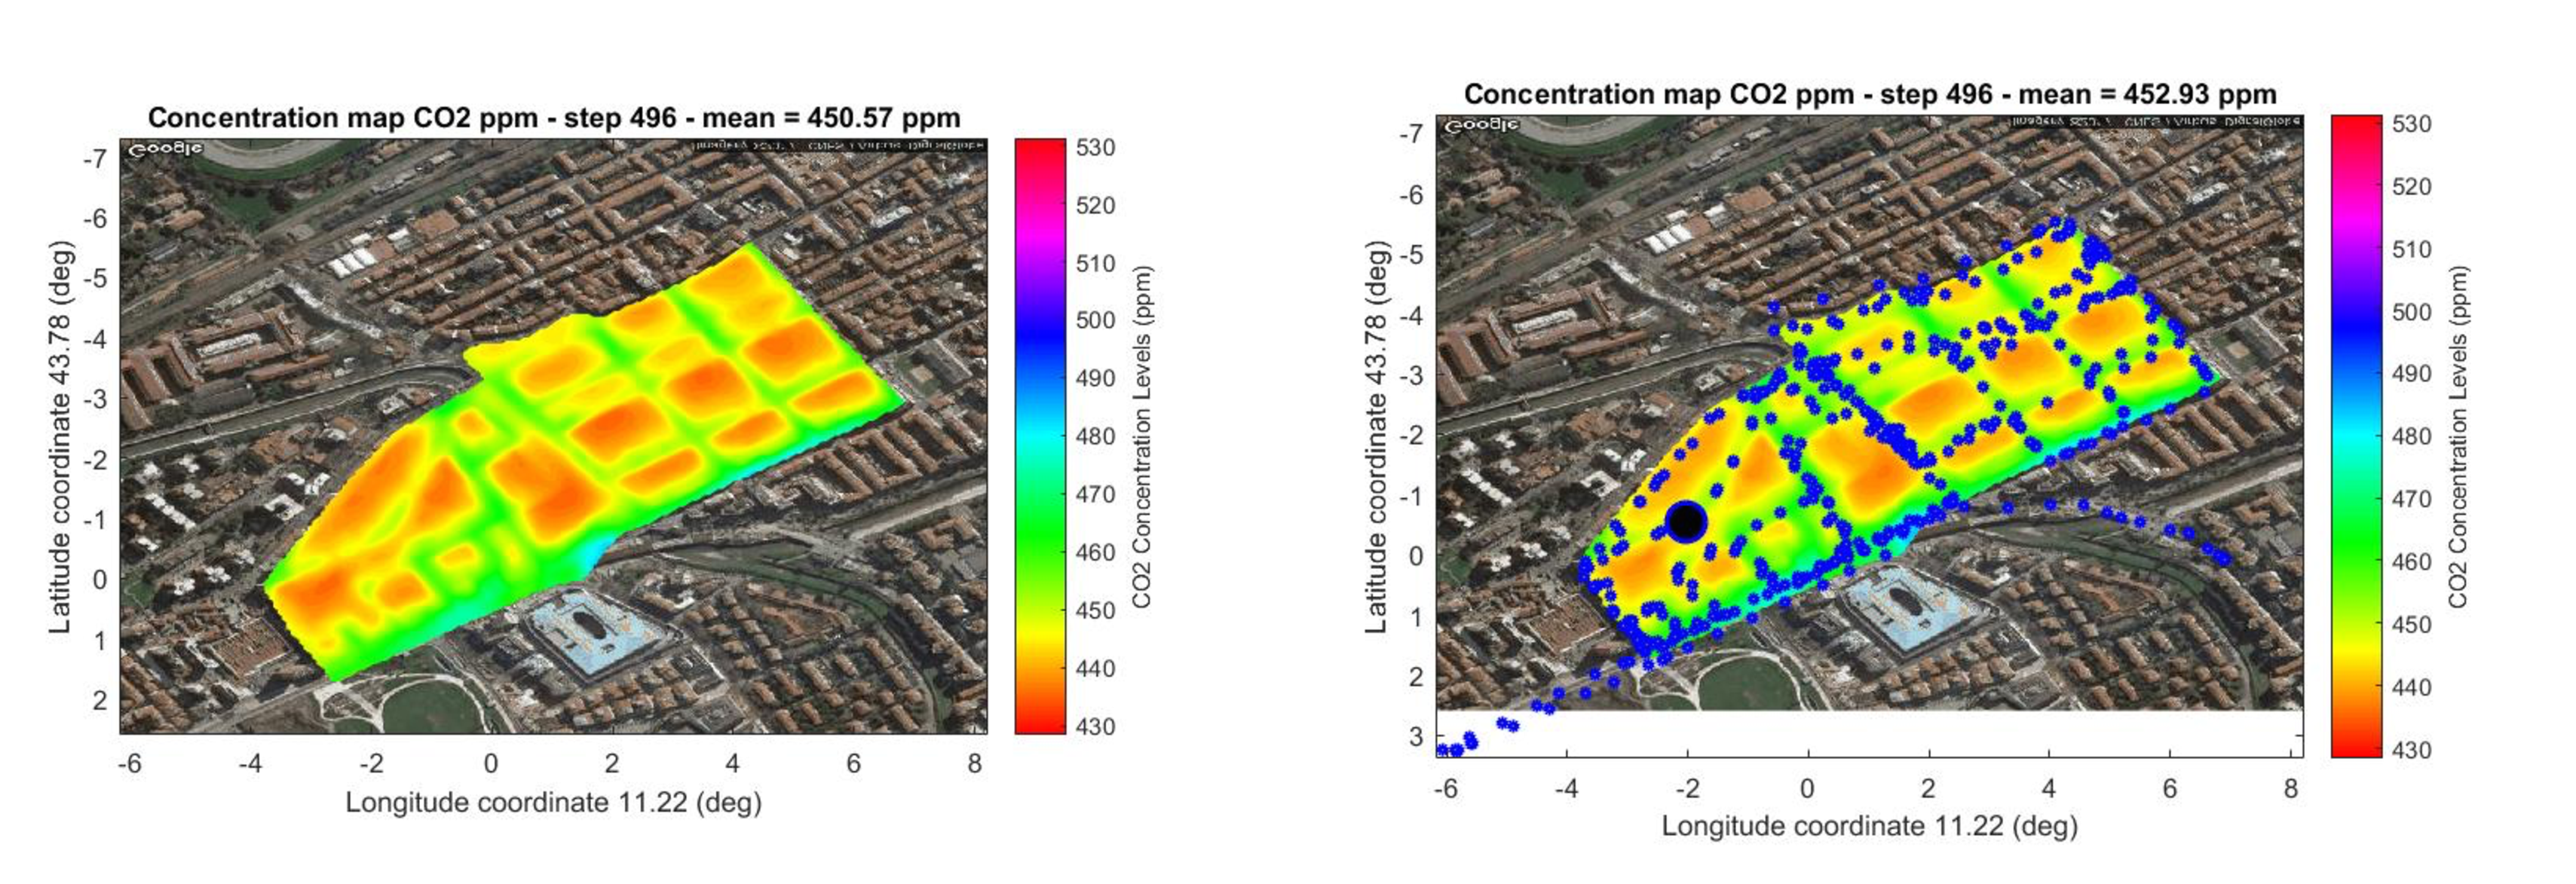
\includegraphics[width=1\columnwidth]{figure/step496}}
	
	\subfloat[]{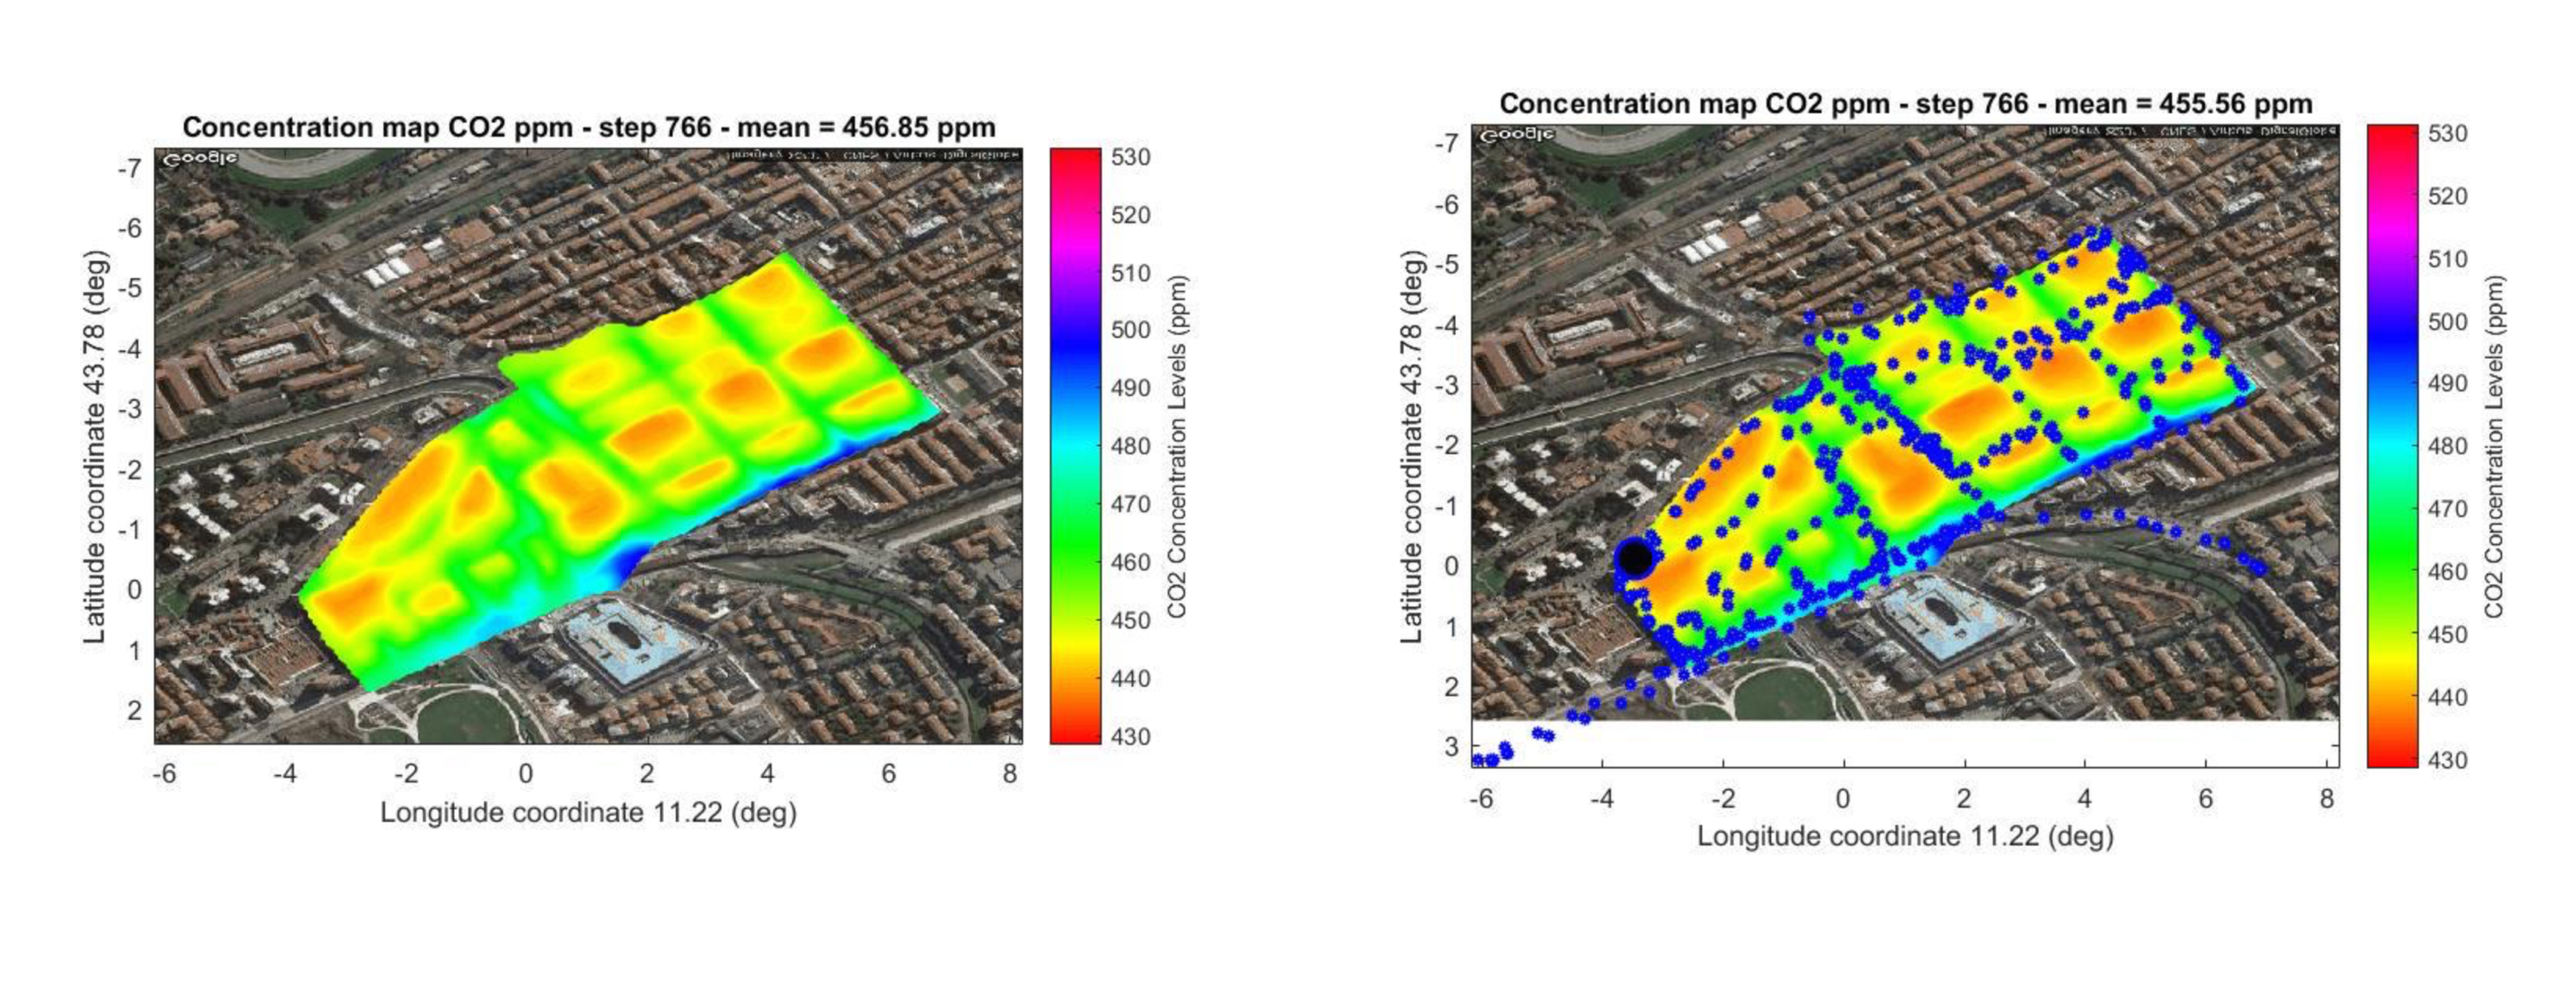
\includegraphics[width=1\columnwidth]{figure/step766}}
\caption{Performance evaluation on simulated data: 2D comparisons of simulated CO$_2$ concentration field (left) and estimated field (right) at difference time instants.} \label{fig:sim_fil_comparison}
\end{figure}

\section{Experimental results}
In this section, we present experimental results concerning the estimation of the concentration field from the data collected in the two measurement campaigns described in Section 6.
For the first measurement campaign, results concerning estimation of CO$_2$ concentration field in the area of interest are provided, and the parameters used in the filter are the same as those use
in the performance evaluation on simulated data of Section 7  (see Table \ref{tab:Parameter_simulation_q150}); conversely, for the second measurement campaign, we have considered the problem of
estimating the CO concentration field and the filter parameters have been chosen as shown in Table \ref{tab:Parameter_simulation_scm_2}.
%%%%%%%%%%%TABLE
\begin{table}[tbp]
 \centering
 \begin{center}  
  \begin{tabular}{|c|c|c|c|c|}
\hline
  $N_T$ & $|\mathcal{K}|$ & $\sigma_{q}^{2}$ & $R_k$ & $\Delta$\\  \hline
 2500 & 772 & $25^2$ & $3^2$ & $10$ \\
\hline
  \end{tabular}
\end{center}  
\caption{Parameters used in the data assimilation algorithm for the second measurement campaign.}
  \label{tab:Parameter_simulation_scm_2}
\end{table}
%%%%%%%END TABLE

Since, in this case, the true concentration field is unknown the TA-RMSE and SA-RMSE cannot be computed. Hence, the P-RMSE of equation \eqref{eq:rmse_meas_4_4} is used as performance criterium
in order to evaluate the performance of the data assimilation algorithm. Fig. \ref{fig:rmse_real_mes1} provides the time behavior of the P-RMSE computed in the scenario corresponding to the first measurement campaign. The P-RMSEs, for each single sensor as well as considering all the sensors together, in the scenario corresponding to the second measurement
campaign are depicted in Fig. \ref{fig:rmse_real_mes2}.
The predictions provided by the data assimilation algorithm are also compared with the true measurements by means of regression functions as shown in Figure \ref{fig:regression_real_truth}.
Finally, the estimated concentration fields of CO$_2$ (first measurement campaign) and CO (second measurement campaign) pollutants at difference time instants are shown in Figures \ref{fig:co2_real_field} and \ref{fig:co_real_field}, respectively. From the examination of the obtained results, the following general conclusions can be drawn:
\begin{itemize}
\item From Figs. \ref{fig:rmse_real_mes1}-\ref{fig:rmse_real_mes2}, we can observe that the difference between measurements $\mb{y}_{k}$ and predictions $\hat{\mb{y}}_{k|k-1}$ is small. Further, for the first measurement campaign such a difference is comparable to the difference found in the simulated scenario of Section 7. This result indicates that the estimated concentration field allows one to accurately predict the future measurements, and hence the estimates can be considered reliable.
\item In both assimilation processes, estimates of pollutant concentration meet expectations. Indeed these values are on average higher along the roads, and smaller in the background or in the buildings.
\item The time variation of the pollutant concentration is in good agreement with the observed traffic intensity. For instance, in the second measurement campaign, the concentration is higher at the beginning and the end, and instead lower in the middle segment.
\end{itemize}



\begin{figure}[p]
\hspace*{-1cm} 
	\centering
	\subfloat[]{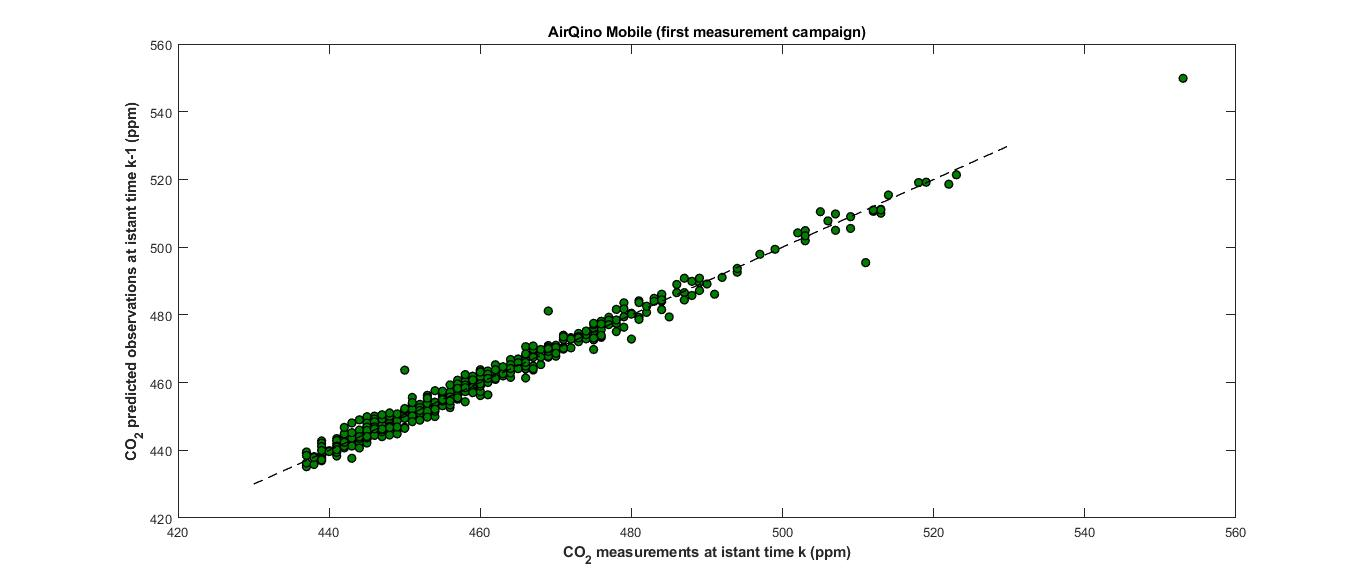
\includegraphics[width=1.1\columnwidth]{figure/error_meas_pred_regression_5.jpg}
		\label{fig:nodes_triangle_2D}}
	\hfil
\hspace*{-1cm} 
	\subfloat[]{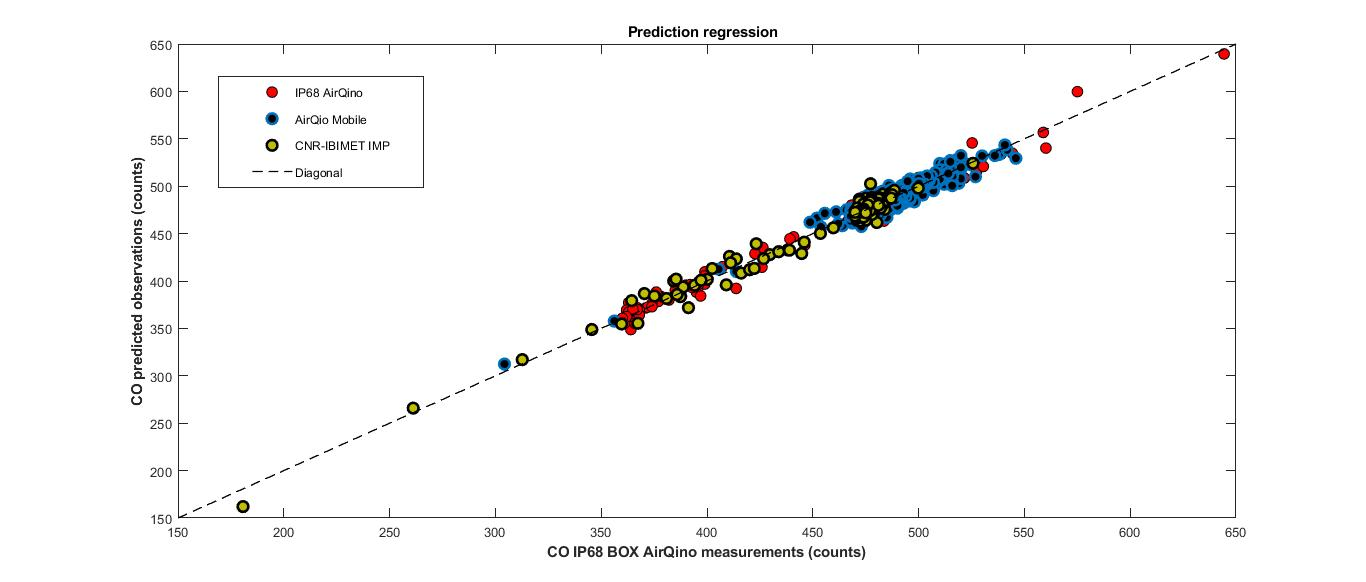
\includegraphics[width=1.1\columnwidth]{figure/sens_TOT_reg.jpg}
		\label{fig:nodes_tetra_3D}}
\phantomcaption
	\caption{Measurement campaigns:  regression functions comparing the measured pollutant concentration and the corresponding prediction $\hat{y}_{k|k-1}$ in the first (a) and second (b) measurement campaign. For the second measurement campaign, the comparison refers to all the three available sensors.}
	\label{fig:regression_real_truth}
\end{figure}
%%%%%%%%%%%%%%%%%%%%%%%%%%%%%%%%
%%%%%%%%%%%%%%%%%%%%%%%%%%%%%%%%%%%%%%%%%%%%%
%%%%%%%%%%%%%%%%%%%%%%%%%%%%%%%%
%%%%%%%%%%%%%%%%%%%%%%%%%%%%%%%%%%%%%%%%%%%%%
%________________________________________________________________________________RMSE
%%%%%%%%%%%%%%%%%%%%%%%%%%%%%%%% RMSE
\begin{figure}[p]
\hspace*{-1cm} 
	\centering
	\subfloat[]{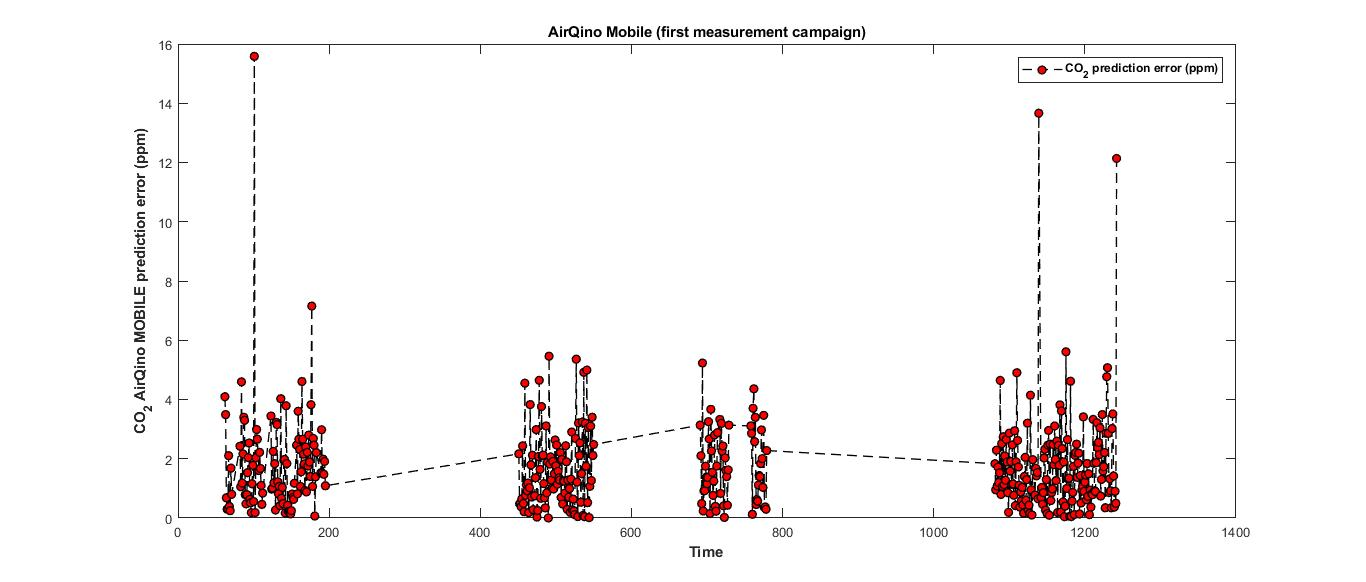
\includegraphics[width=1.1\columnwidth]{figure/error_meas_pred_4.jpg}
		\label{fig:nodes_triangle_2D}}
\hfil
	\caption{First measurement campaign: time behavior of the P-RMSE between the measured CO$_2$ concentration values and the predictions of the data assimilation algorithm.}
	\label{fig:rmse_real_mes1}
\end{figure}
%%%%%%%%%%%%%%%%%%%%%%%%%%%%%%%%%%%%%%%%%%%%%
\begin{figure}[p]\ContinuedFloat
\hspace*{-1cm}  
	\centering
	\subfloat[]{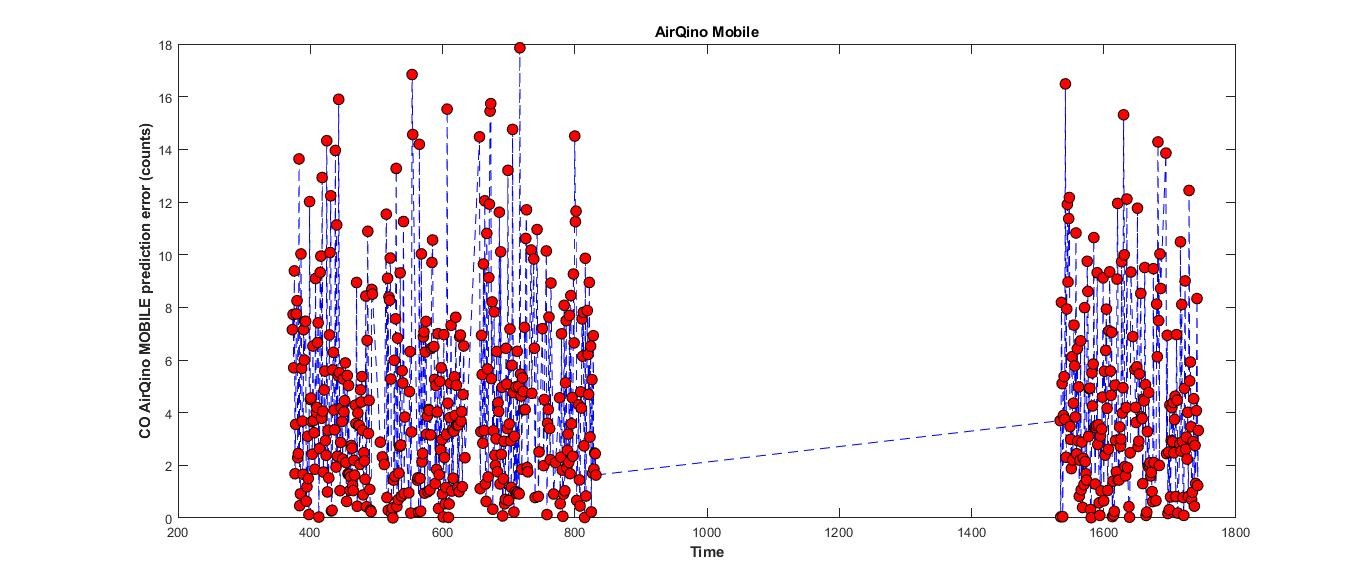
\includegraphics[width=1.1\columnwidth]{figure/sens_1_error.jpg}
		\label{fig:nodes_triangle_2D}}
	\hfil
\hspace*{-1cm} 
	\subfloat[]{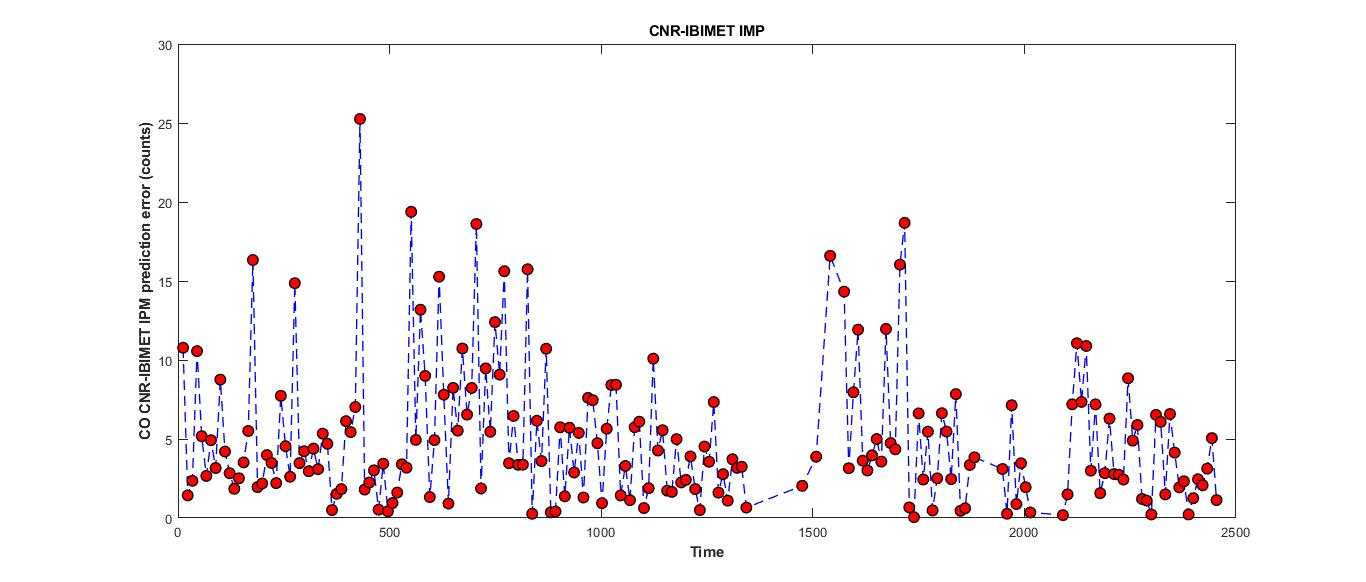
\includegraphics[width=1.1\columnwidth]{figure/sens_2_error.jpg}
		\label{fig:nodes_tetra_3D}}
\hfill
\hspace*{-1cm} 
	\centering
	\subfloat[]{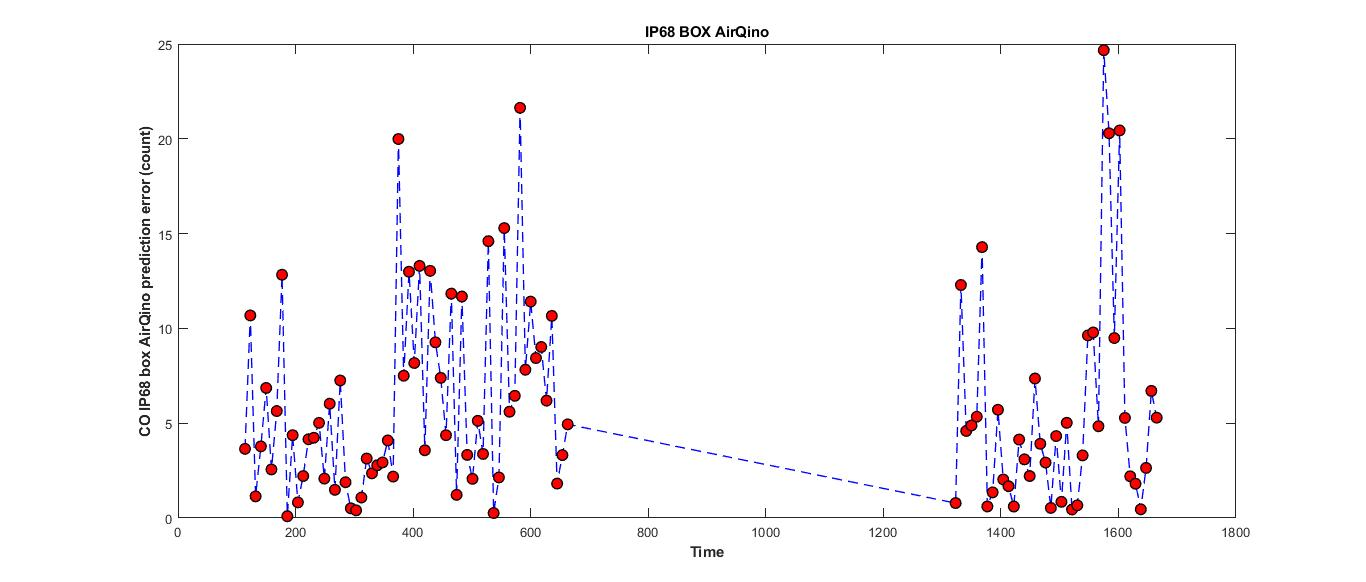
\includegraphics[width=1.1\columnwidth]{figure/sens_3_error.jpg}
		\label{fig:nodes_triangle_2D}}
	\hfil
\hspace*{-1cm} 
	\subfloat[]{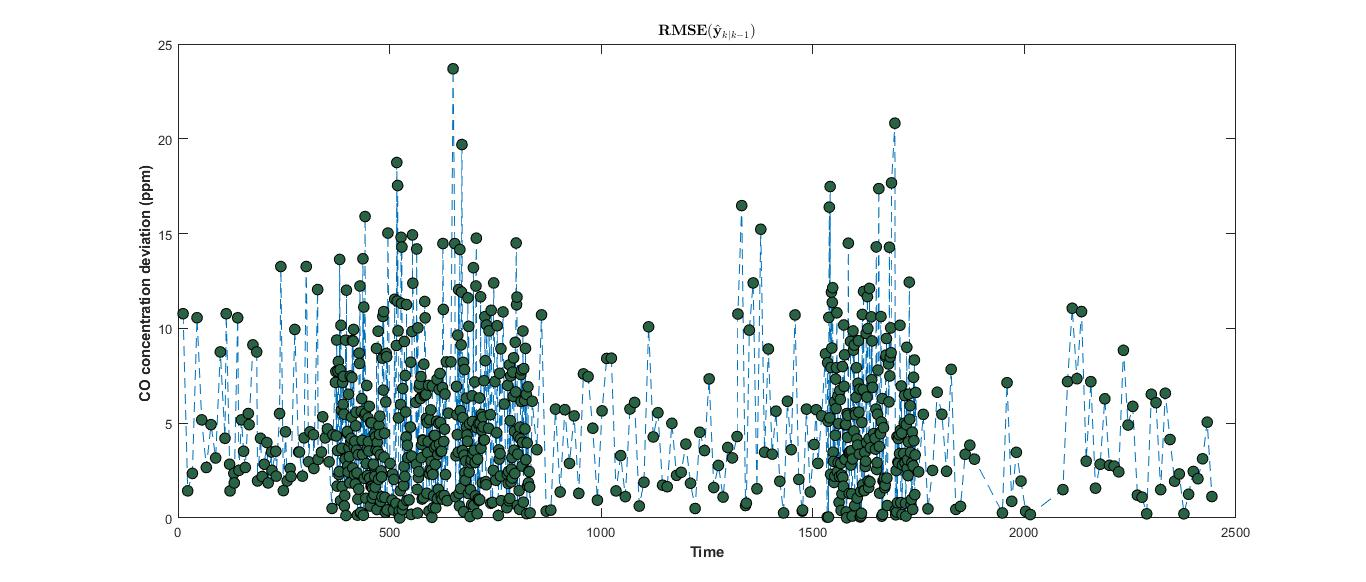
\includegraphics[width=1.1\columnwidth]{figure/sens_tot_error_rmse.jpg}
		\label{fig:nodes_tetra_3D}}
\phantomcaption
\phantomcaption
	\caption{Second measurement campaign: time behavior of the P-RMSE between the measured CO concentration values and the predictions of the data assimilation algorithm computed for each sensor
(a),(b),(c) and considering all the sensors together (d).}
	\label{fig:rmse_real_mes2}
\end{figure}
%%%%%%%%%%%%%%%%%%%%%%%%%%%%%%%%
%%%%%%%%%%%%%%%%%%%%%%%%%%%%%%%%%%%%%%%%%%%%%C02 CONCENTRATION FIELD
%%%%%%%%%%%%%%%%%%%%%%%%%%%%%%%% 
\begin{figure}[h!]
\hspace*{-1cm} 
	\centering
	\subfloat[]{\includegraphics[width=0.6\columnwidth]{figure/filename_co2_DR_62.jpg}
		\label{fig:nodes_triangle_2D}}
	\centering
	\subfloat[]{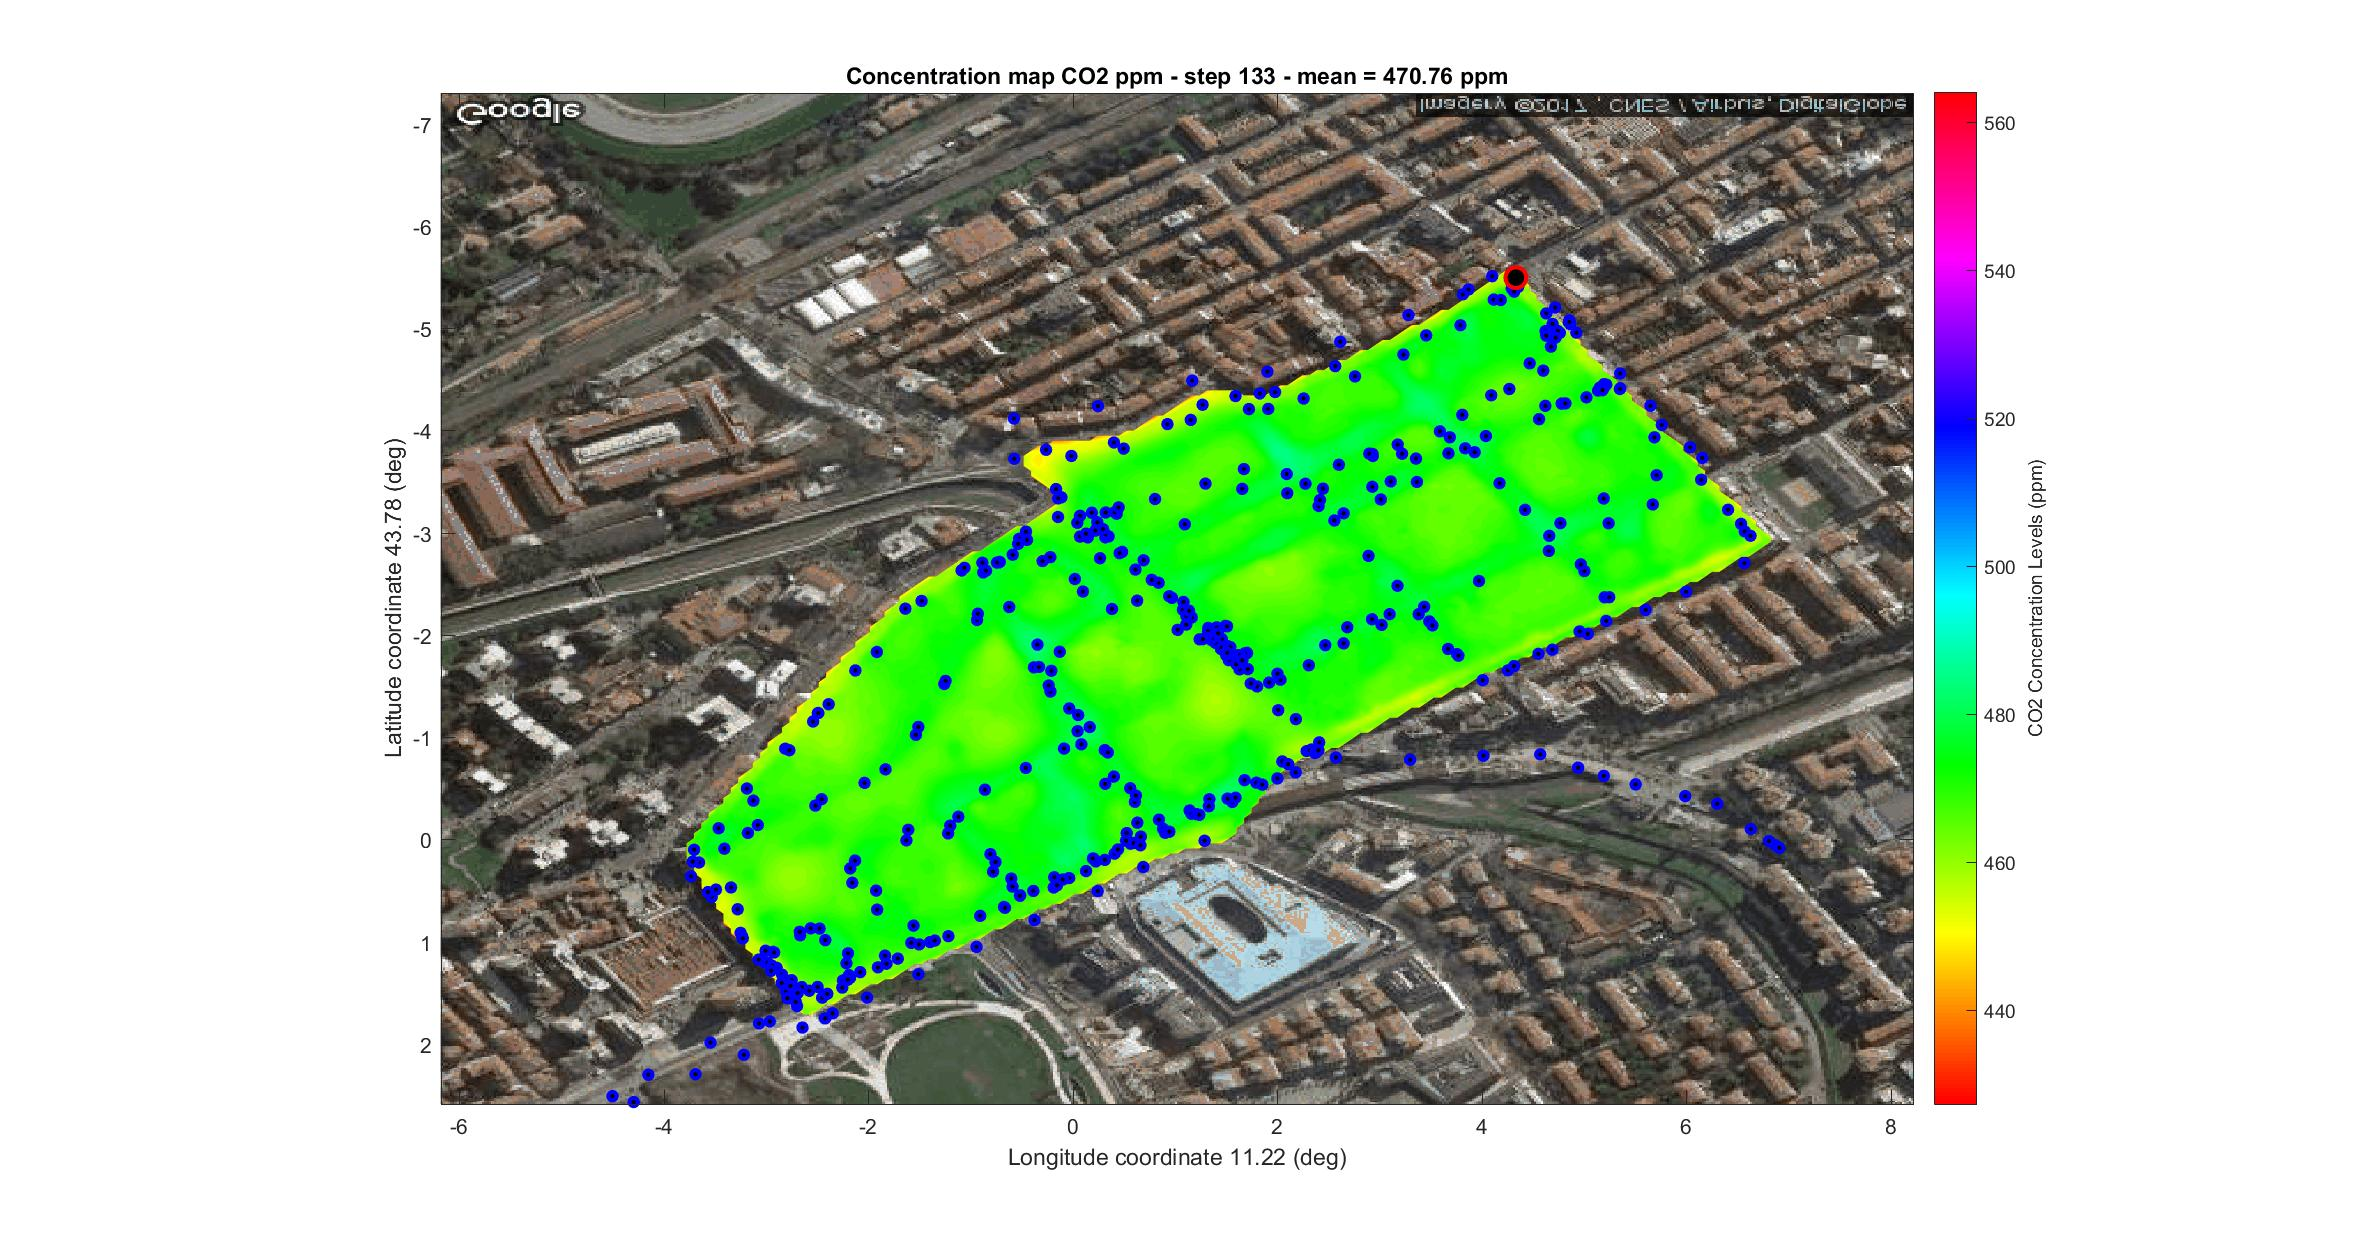
\includegraphics[width=0.6\columnwidth]{figure/filename_co2_DR_133.jpg}
		\label{fig:nodes_triangle_2D}}\hfil
\hspace*{-1cm} 
	\subfloat[]{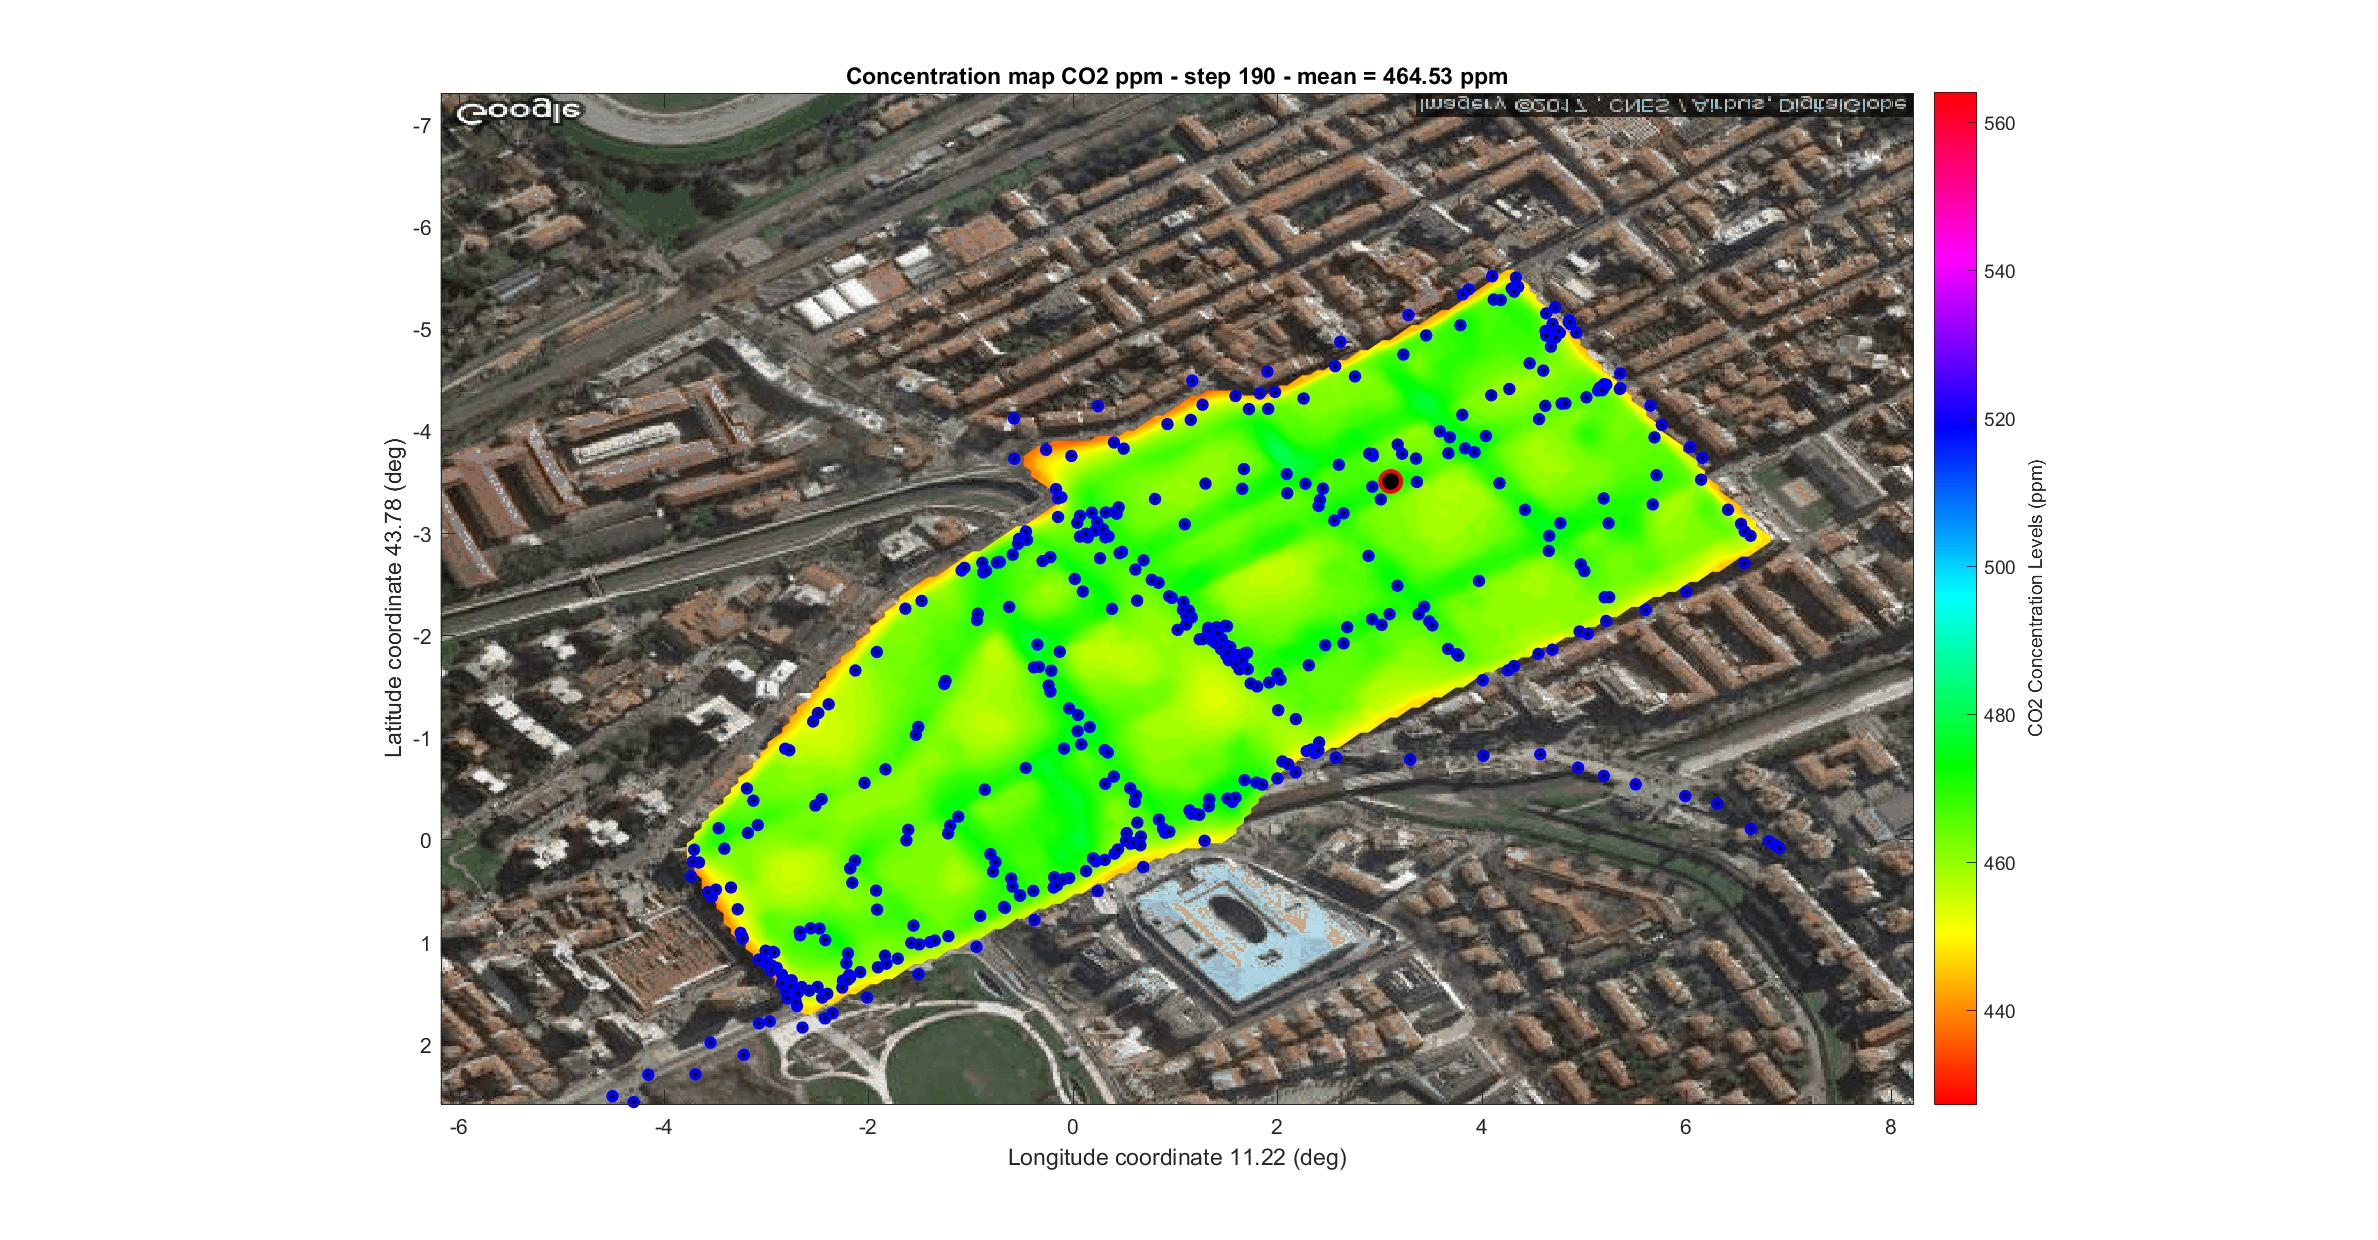
\includegraphics[width=0.6\columnwidth]{figure/filename_co2_DR_190.jpg}
		\label{fig:nodes_tetra_3D}}
	\subfloat[]{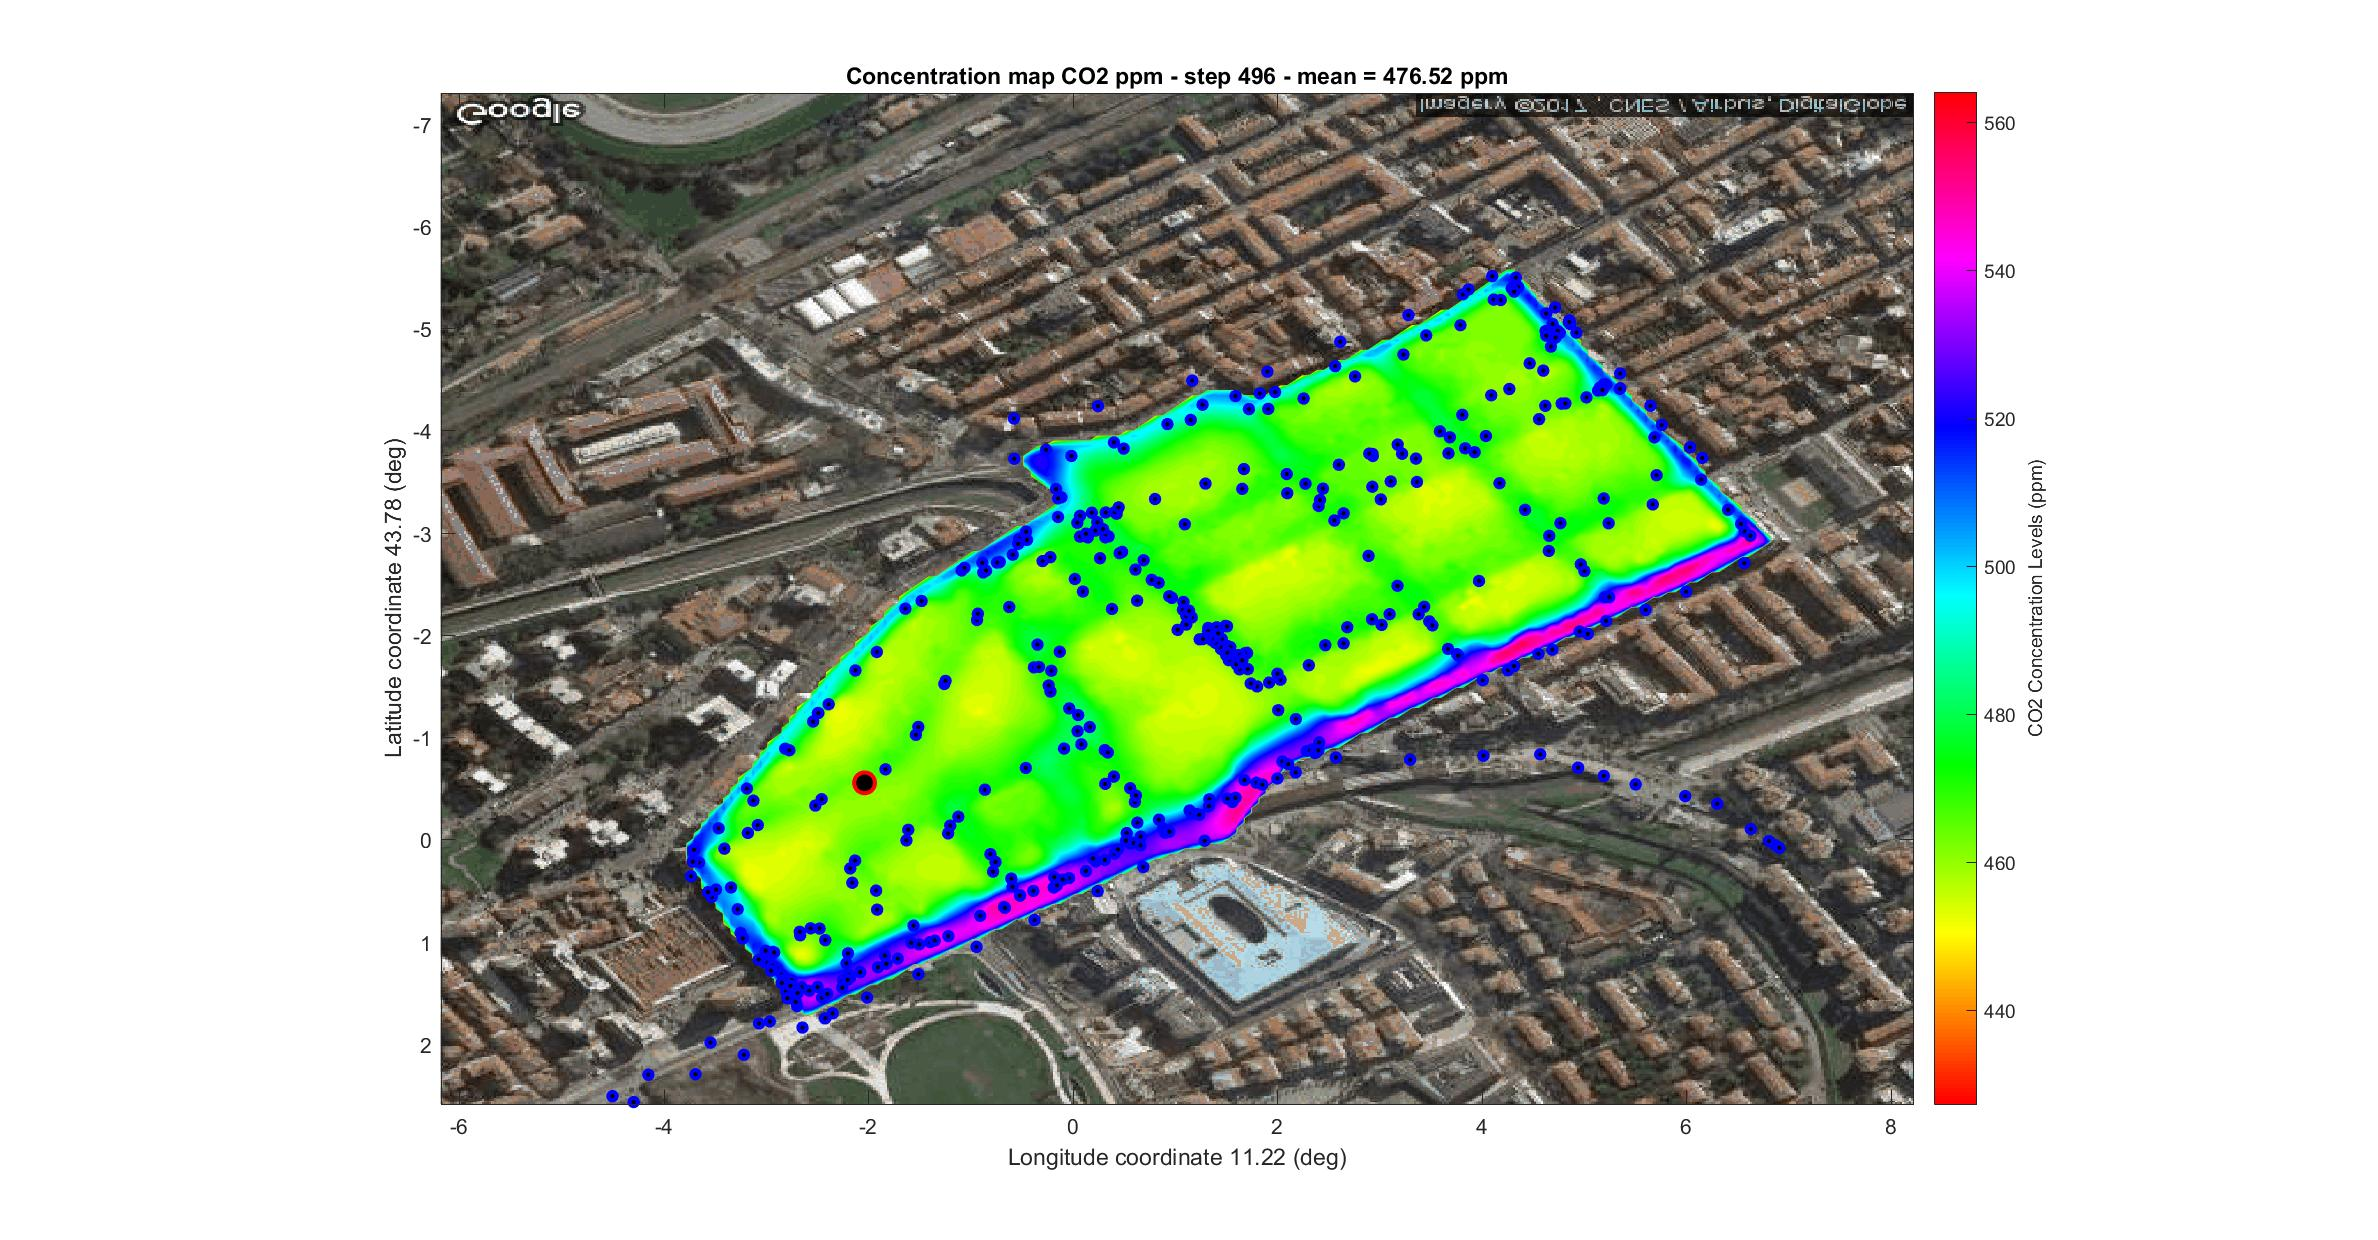
\includegraphics[width=0.6\columnwidth]{figure/filename_co2_DR_496.jpg}
		\label{fig:nodes_triangle_2D}}
	%\hfil
%\hspace*{-3cm} 
	%\subfloat[]{\includegraphics[width=1.5\columnwidth]{figure/chp7/filename_co2_DR_62.jpg}
		%\label{fig:nodes_tetra_3D}}
	\caption{First measurement campaign: estimated CO$_2$ concentration field at different time instants.}
	\label{fig:co2_real_field}
\end{figure}

%%%%%%%%%%%%%%%%%%%%%%%%%%%%%%%%%%%%%%%%%%%%%
\begin{figure}[p]
\hspace*{-1.2cm}  
	\centering
	\subfloat[]{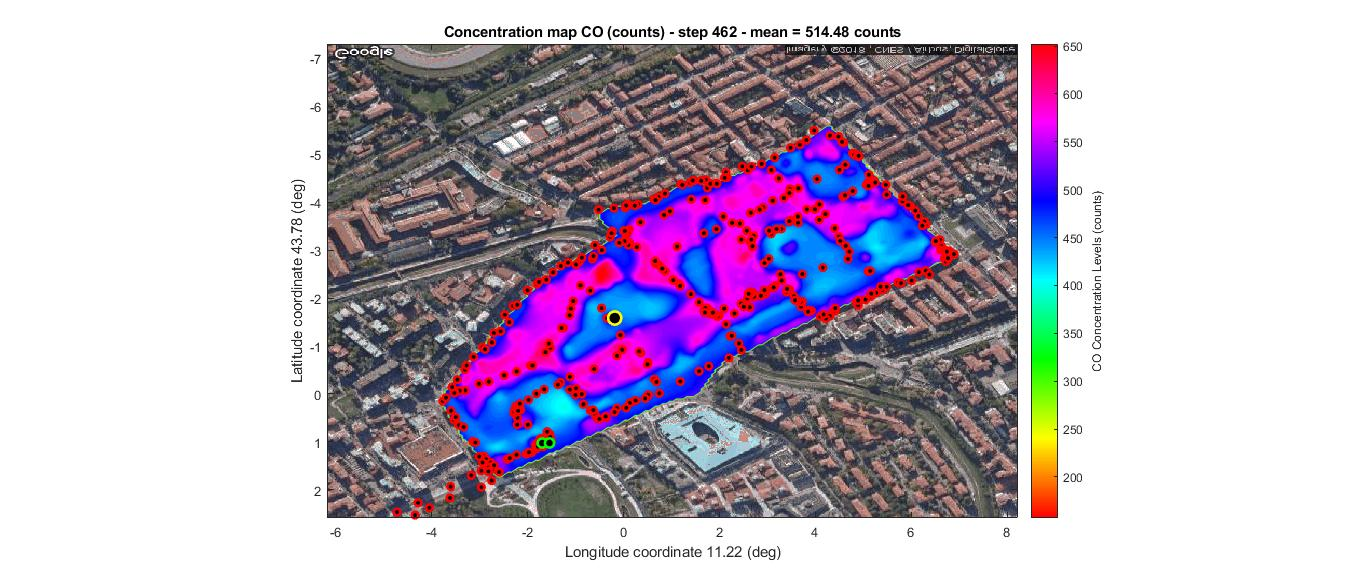
\includegraphics[width=0.7\columnwidth]{figure/filename_462.jpg}
		\label{fig:nodes_triangle_2D}}
	\subfloat[]{\hspace{-2cm}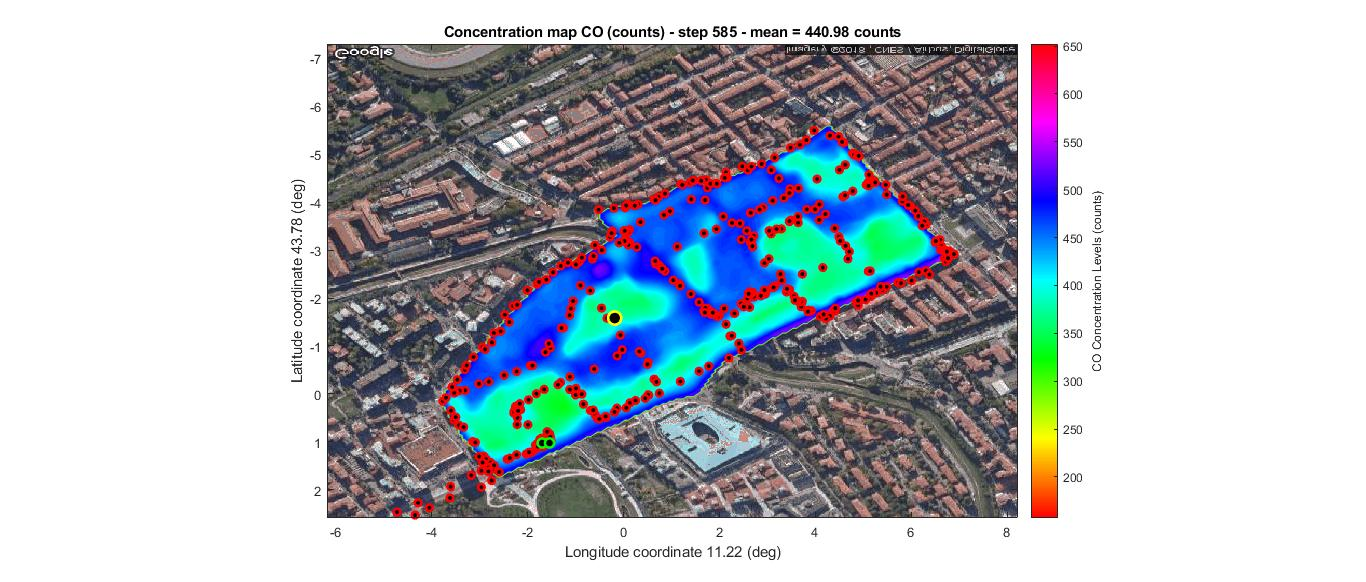
\includegraphics[width=0.7\columnwidth]{figure/filename_585.jpg}
		\label{fig:nodes_triangle_2D}}
	\hfil
\hspace*{-1.2cm} 
	\centering
	\subfloat[]{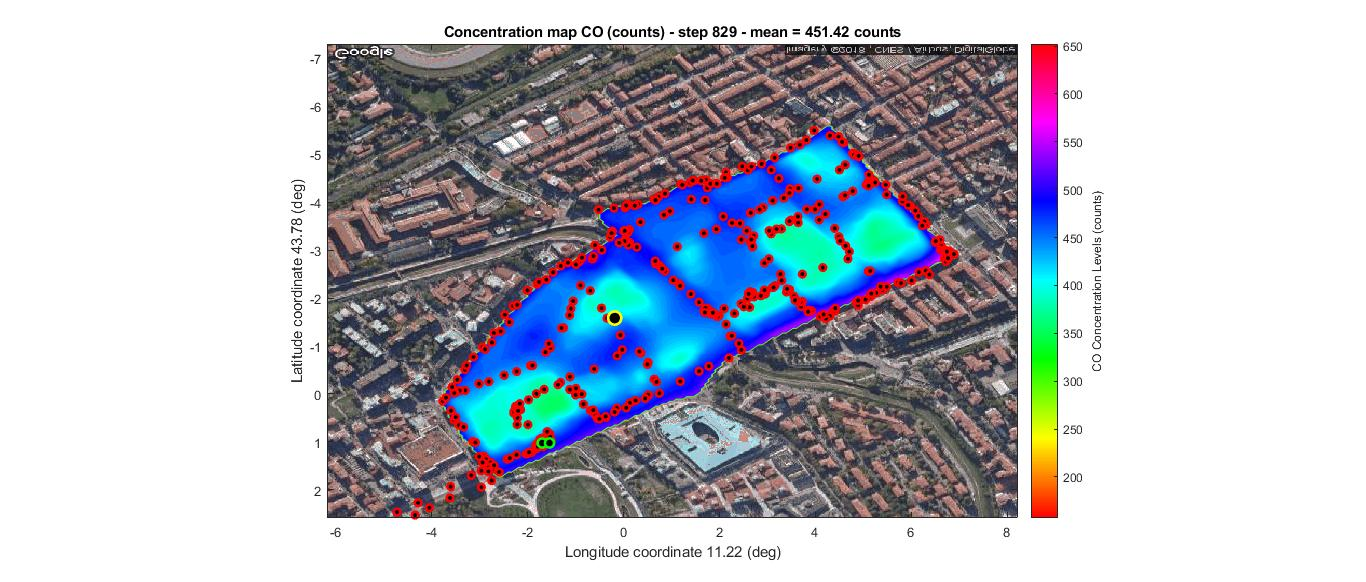
\includegraphics[width=0.7\columnwidth]{figure/filename_829.jpg}
		\label{fig:nodes_triangle_2D}}
	\subfloat[]{\hspace{-2cm}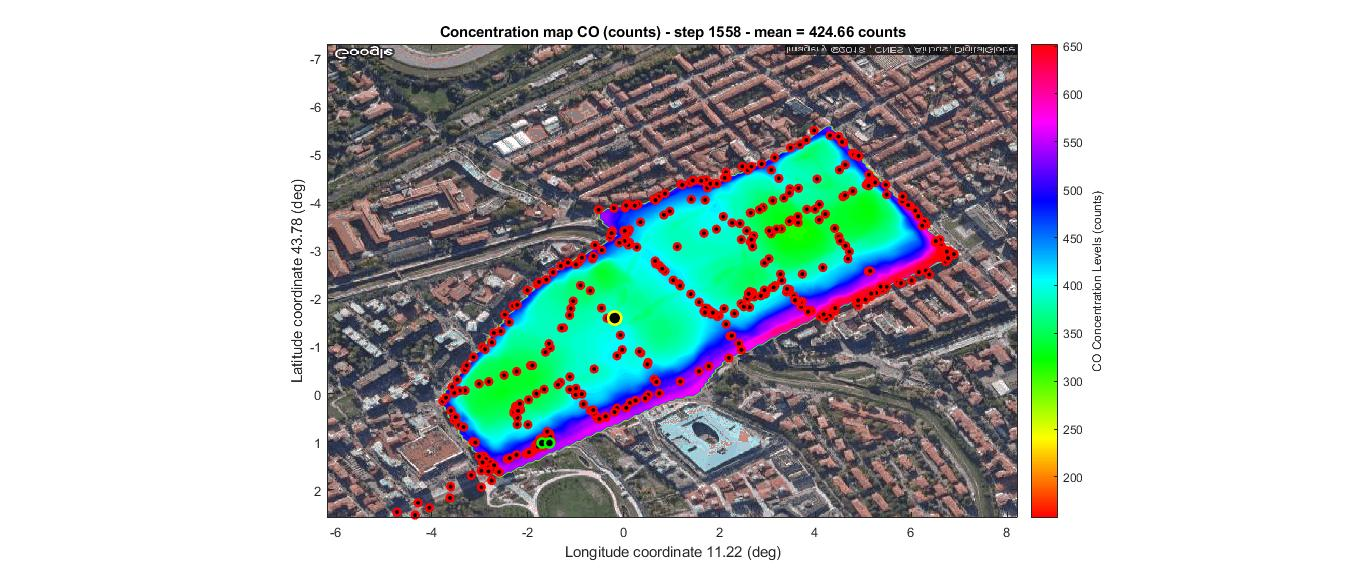
\includegraphics[width=0.7\columnwidth]{figure/filename_1558.jpg}
		\label{fig:nodes_triangle_2D}}
	\hfil
\hspace*{-1.2cm} 
\centering
	\subfloat[]{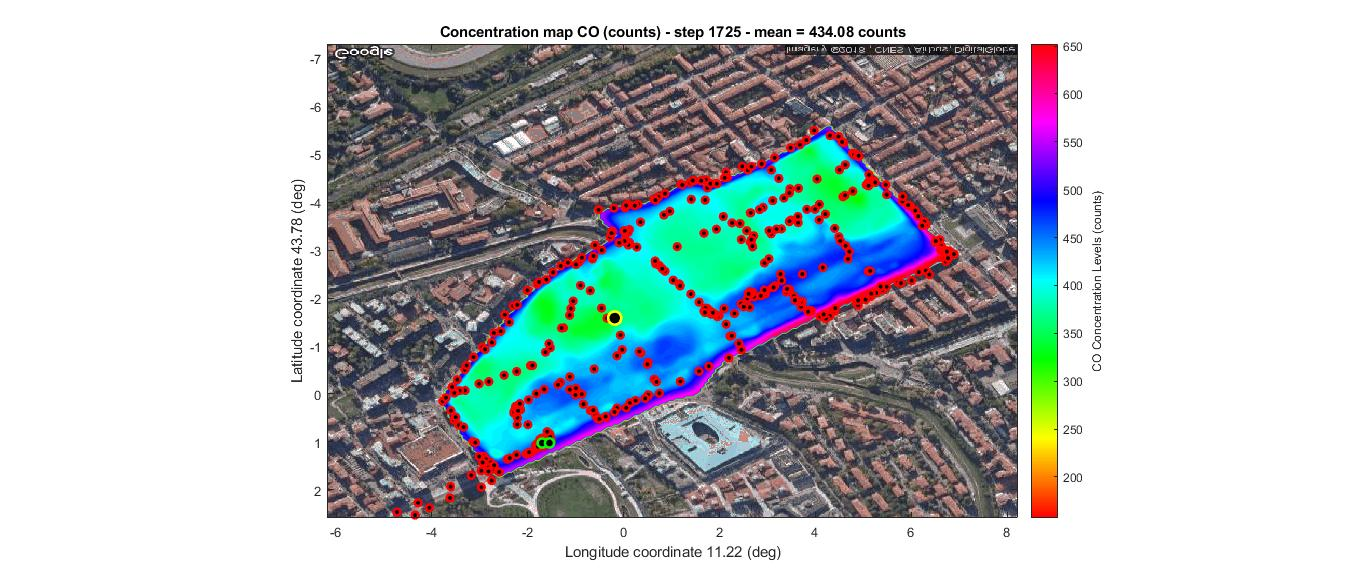
\includegraphics[width=0.7\columnwidth]{figure/filename_1725.jpg}
		\label{fig:nodes_tetra_3D}}
	\subfloat[]{\hspace{-2cm}\includegraphics[width=0.7\columnwidth]{figure/filename_2212.jpg}
		\label{fig:nodes_triangle_2D}}
	%\hfil
%\hspace*{-3cm} 
	%\subfloat[]{\includegraphics[width=1.5\columnwidth]{figure/chp7/filename_co2_DR_62.jpg}
		%\label{fig:nodes_tetra_3D}}
	\caption{Second measurement campaign: estimated CO concentration field at different time instants.}
	\label{fig:co_real_field}
\end{figure}




\section{Conclusion}
The project has addressed high-resolution air quality monitoring in an urban environment
exploiting data assimilation techniques that combine mathematical
modeling of the pollutant dispersion dynamics along with pointwise-in-time-and-
space pollutant concentration measurements provided by appropriate
sensors. In particular, the project has led to the complete software development
of a data-assimilation system and to its pilot application to air
quality monitoring of a given area in the city of Florence. The developed
system exploited the following ingredients: Advection-Diffusion (AD) Partial Differential equation (PDE)
for air pollution modeling; Finite Element Method (FEM) for spatial discretization of the AD
PDE into a finite-dimensional large-scale continuous-time state-space
model; time-discretization to obtain a discrete-time state space model;
use of meteo and vehicular traffic data for tuning the model parameters
and computing input emissions;
Ensemble Kalman Filter (EnKF) for computationally efficient data assimilation with a large-scale model;
low-cost mobile and/or fixed AirQino boards, developed by IBIMET-CNR,
for measuring concentrations of several pollutants and air temperature
as well as radio transmitting geolocated measurements to the
data assimilation center.
The effectiveness of the system, in terms of accurate space-time reconstruction
of the pollutant concentration map, has been successfully tested via both
computer-simulated and real data, the latter collected through
data-acquisition campaigns with fixed and/or mobile sensors located in the
area of interest.

Possible directions for future works are: creation of a network of sensors covering the whole urban area;
creation of a network of IMP platforms in critical points in the city so as to combine air quality measurements with measurements of vehicle
flows divided by vehicle classes; active involvement of citizens in air quality  monitoring (citizen
science); real-time strategies for pollution exposure control;
automatic control systems for lowering the level of pollution (for example,
pollutant suction filters positioned at critical points);
intelligent control systems for traffic sorting, regulated by the level of
pollution.






% if have a single appendix:
%\appendix[Proof of the Zonklar Equations]
% or
%\appendix  % for no appendix heading
% do not use \section anymore after \appendix, only \section*
% is possibly needed

% use appendices with more than one appendix
% then use \section to start each appendix
% you must declare a \section before using any
% \subsection or using \label (\appendices by itself
% starts a section numbered zero.)
%


%\appendices
%\section{Proof of the First Zonklar Equation}
%Appendix one text goes here.

% you can choose not to have a title for an appendix
% if you want by leaving the argument blank
%\section{}
%Appendix two text goes here.
%

% use section* for acknowledgment
\section*{Acknowledgment}
The authors would like to thank \textit{Fondazione Cassa di Risparmio Firenze} for the financial support of this project;
all the people involved in the project and particularly Lin Gao, Suqi Li, and Bailu Wang; Alessandro Zaldei of IBIMET-CNR
for providing us the sensors used in the measurement campaigns; Alice Cavaliere, Sara Di Lonardo, and Lapo Frascati for helping with the measurement campaigns.




% Can use something like this to put references on a page
% by themselves when using endfloat and the captionsoff option.
\ifCLASSOPTIONcaptionsoff
  \newpage
\fi



% trigger a \newpage just before the given reference
% number - used to balance the columns on the last page
% adjust value as needed - may need to be readjusted if
% the document is modified later
%\IEEEtriggeratref{8}
% The "triggered" command can be changed if desired:
%\IEEEtriggercmd{\enlargethispage{-5in}}

% references section

% can use a bibliography generated by BibTeX as a .bbl file
% BibTeX documentation can be easily obtained at:
% http://mirror.ctan.org/biblio/bibtex/contrib/doc/
% The IEEEtran BibTeX style support page is at:
% http://www.michaelshell.org/tex/ieeetran/bibtex/
%\bibliographystyle{IEEEtran}
% argument is your BibTeX string definitions and bibliography database(s)
%\bibliography{IEEEabrv,../bib/paper}
%
% <OR> manually copy in the resultant .bbl file
% set second argument of \begin to the number of references
% (used to reserve space for the reference number labels box)
\begin{thebibliography}{99}
\bibitem{bib:MEET001}
{\em {Transport Research Laboratory, Project Report SE/491/98, Methodology for
  calculating transport emissions and energy consumption, Edited by A. J.
  Hickman}}.

\bibitem{TheLancetComm01}
{ P. J. Landrigan, R. Fuller, N. J. Acosta, O. Adeyi, R. Arnold, A. B. Bald\'e
  , R. Bertollini, S. Bose-O'Reilly, J. I. Boufford, P. N. Breysse, et al.
  \textit{The Lancet Commision on pollution and health}}.
\newblock {\em The Lancet}, 2017.

\bibitem{bib:neuralgasindian}
{A. K. Das1, A. K. Patnaik, A. N. Dehury, P. K. Bhuyan, U. Chattaraj and M.
  Panda}.
\newblock {Defining Level of Service Criteria of Urban Streets Using Neural Gas
  Clustering}.
\newblock {\em IOSR Journal of Engineering (IOSRJEN)}, 3(5):18--25, {May,
  2013}.

\bibitem{bib:alicavphd06}
{A. Zaldei, F. Camilli, T. De Filippis, F. Di Gennaro, S. Di Lonardo, F. Dini,
  B. Gioli, G.i Gualtieri, A. Matese, W. Nunziati, et al. An integrated
  low-cost road traffic and air pollution monitoring platform for next citizen
  observatories. \textit{Transportation research procedia}, 24:531-538, 2017.}

\bibitem{TAC}
G.~Battistelli, L.~Chisci, N.~Forti, G.~Pelosi, and S.~Selleri.
\newblock Distributed finite-element kalman filter for field estimation.
\newblock {\em IEEE Transactions on Automatic Control}, 62(7):3309--3322, 2017.

\bibitem{cavaliere01}
Alice Cavaliere.
\newblock {\em Low-cost air quality stations and control networks for a smart
  city}.
\newblock PhD thesis, University of Florence, 2017.

\bibitem{OccandEnvMed01}
Kai~Jen Chuang, Yuan~Horng Yan, Shu~Yi Chiu, and Tsun-Jen Cheng.
\newblock {Longterm air pollution exposure and risk factors for cardiovascular
  diseases among the elderly in Taiwan}.
\newblock {\em Occupational and Environmental Medicine}, 1(68):64--68, 2014.

\bibitem{TSIPN}
N.~Forti, G.~Battistelli, L.~Chisci, S.~Li, B.~Wang, and B.~Sinopoli.
\newblock Distributed joint attack detection and secure state estimation.
\newblock {\em IEEE Transactions on Signal and Information Processing over
  Networks}, 2018.

\bibitem{Gander08}
Martin~J. Gander.
\newblock Schwarz methods over the course of time.
\newblock {\em ETNA. Electronic Transactions on Numerical Analysis},
  31:228--255, 2008.

\bibitem{GuFoDLe01}
Cristina B~B Guerreiro, Valentin Foltescu, and Frank~De Leeuw.
\newblock {Air quality status and trends in Europe}.
\newblock {\em Atmospheric environment}, (98):376--384, 2014.

\bibitem{Lions88}
P.L. Lions.
\newblock On the {S}chwarz alternating method. {I}.
\newblock In {\em First Int. Symp. on Domain Decomposition Methods for Partial
  Differential Equations}, pages 1--142, 1988.

\bibitem{Massman_001}
W.~J. Massman.
\newblock A review of the molecular diffusivities of {H$_2$O}, {CO$_2$},
  {CH$_4$}, {CO}, {O3}, {SO$_2$}, {NH$_3$}, {N$_2$O}, {NO}, and {NO$_2$} in
  air, {O$_2$} and {PN$_2$} near stp.
\newblock {\em Atmospheric Environment}, 32(16):1111--1127, March 1998.

\bibitem{Pelosi09}
G.~Pelosi, R.~Coccioli, and S.~Selleri.
\newblock {\em Quick finite elements for electromagnetic waves}.
\newblock Artech House, 2009.

\bibitem{Silv96}
P.P. Silvester and R.L. Ferrari.
\newblock {\em Finite elements for electrical engineers}.
\newblock Cambridge University Press, 1996.
%\bibitem{IEEEhowto:kopka}
%H.~Kopka and P.~W. Daly, \emph{A Guide to \LaTeX}, 3rd~ed.\hskip 1em plus
%  0.5em minus 0.4em\relax Harlow, England: Addison-Wesley, 1999.
%
\end{thebibliography}

% biography section
% 
% If you have an EPS/PDF photo (graphicx package needed) extra braces are
% needed around the contents of the optional argument to biography to prevent
% the LaTeX parser from getting confused when it sees the complicated
% \includegraphics command within an optional argument. (You could create
% your own custom macro containing the \includegraphics command to make things
% simpler here.)
%\begin{IEEEbiography}[{\includegraphics[width=1in,height=1.25in,clip,keepaspectratio]{mshell}}]{Michael Shell}
% or if you just want to reserve a space for a photo:

%\begin{IEEEbiography}{Michael Shell}
%Biography text here.
%\end{IEEEbiography}
%
%% if you will not have a photo at all:
%\begin{IEEEbiographynophoto}{John Doe}
%Biography text here.
%\end{IEEEbiographynophoto}
%
%% insert where needed to balance the two columns on the last page with
%% biographies
%%\newpage
%
%\begin{IEEEbiographynophoto}{Jane Doe}
%Biography text here.
%\end{IEEEbiographynophoto}
%
% You can push biographies down or up by placing
% a \vfill before or after them. The appropriate
% use of \vfill depends on what kind of text is
% on the last page and whether or not the columns
% are being equalized.

%\vfill

% Can be used to pull up biographies so that the bottom of the last one
% is flush with the other column.
%\enlargethispage{-5in}



% that's all folks
\end{document}


